% !TeX encoding = UTF-8
% !TeX spellcheck = sk_SK
\documentclass[]{tukediphc}
%% -----------------------------------------------------------------
%% tento subor ma kodovanie utf-8
%%
%% na kompilaciu pouzivajte format pdflatex 
%%
%% V pripade problemov kontaktujte Jána Bušu st. (jan.busa@tuke.sk)
%%
%% November 2015
%% -----------------------------------------------------------------
%%
%\usepackage[dvips]{graphicx}
%\DeclareGraphicsExtensions{.eps}
\usepackage[pdftex]{graphicx}
\DeclareGraphicsExtensions{.pdf,.png,.jpg,.mps}
\graphicspath{{figures/}} % priecinok na obrazky
%%


%\usepackage[utf8]{inputenc}  % je v cls-subore
%\usepackage[T1]{fontenc}  % je v cls-subore
\usepackage{lmodern,textcase}
\usepackage[slovak]{babel}
\def\refname{Zoznam použitej literatúry}
\usepackage{latexsym}
\usepackage{dcolumn} % zarovnanie cisiel v tabulke podla des. ciarky
\usepackage{hhline}
\usepackage{amsmath,amsfonts,amssymb}
\usepackage{nicefrac} % pekne zlomky
\usepackage{upgreek} % napr. $\upmu\mathrm{m}$ pre mikrometer ...
\usepackage[final]{showkeys}%color%notref%notcite%final
\usepackage[slovak,noprefix]{nomencl}
\usepackage{parskip}
\usepackage[skip=-6pt]{caption}
\usepackage{mathtools}
\usepackage{standalone}
\makeglossary % prikaz na vytvorenie suboru .glo


% Pouzit v pripade velkeho poctu subsection v tableofcontents
%\makeatletter
%\renewcommand*\l@subsection{\@dottedtocline{2}{1.5em}{3.5em}}
%\newcommand*\l@subsection{\@dottedtocline{2}{1.5em}{2.3em}}
%\newcommand*\l@subsubsection{\@dottedtocline{3}{3.8em}{3.2em}}
%\makeatother


%\def\thefigure{\Roman{section}.\arabic{figure}}

%\usepackage{parskip}% 'zhusti' polozky obsahu
%% Cislovane citovanie
\usepackage[numbers]{natbib}
%%
%% Citovanie podľa mena autora a roku
%\usepackage{natbib} \citestyle{chicago}
% -----------------------------------------------------------------
%% tlač !!!
\usepackage[pdftex,unicode=true,bookmarksnumbered=true,
bookmarksopen=true,pdfmenubar=true,pdfview=Fit,linktocpage=true,
pageanchor=true,bookmarkstype=toc,pdfpagemode=UseOutlines,
pdfstartpage=1]{hyperref}
\usepackage{graphicx}
\usepackage{amsmath}

\PassOptionsToPackage{unicode}{hyperref}
\PassOptionsToPackage{hyphens}{url}
%
\documentclass[]{article}
\usepackage{lmodern}
\usepackage{subfiles}
\usepackage{amssymb,amsmath}
\usepackage{ifxetex,ifluatex}
\ifnum 0\ifxetex 1\fi\ifluatex 1\fi=0 % if pdftex
  \usepackage[T1]{fontenc}
  \usepackage[utf8]{inputenc}
  \usepackage{textcomp} % provide euro and other symbols
\else % if luatex or xetex
  \usepackage{unicode-math}
  \defaultfontfeatures{Scale=MatchLowercase}
  \defaultfontfeatures[\rmfamily]{Ligatures=TeX,Scale=1}
\fi
% Use upquote if available, for straight quotes in verbatim environments
\IfFileExists{upquote.sty}{\usepackage{upquote}}{}
\IfFileExists{microtype.sty}{% use microtype if available
  \usepackage[]{microtype}
  \UseMicrotypeSet[protrusion]{basicmath} % disable protrusion for tt fonts
}{}
\makeatletter
\@ifundefined{KOMAClassName}{% if non-KOMA class
  \IfFileExists{parskip.sty}{%
    \usepackage{parskip}
  }{% else
    \setlength{\parindent}{0pt}
    \setlength{\parskip}{6pt plus 2pt minus 1pt}}
}{% if KOMA class
  \KOMAoptions{parskip=half}}
\makeatother
\usepackage{xcolor}
\IfFileExists{xurl.sty}{\usepackage{xurl}}{} % add URL line breaks if available
\IfFileExists{bookmark.sty}{\usepackage{bookmark}}{\usepackage{hyperref}}
\hypersetup{
  pdftitle={Praktická časť diplomovej práce},
  hidelinks,
  pdfcreator={LaTeX via pandoc}}
\urlstyle{same} % disable monospaced font for URLs
\usepackage[margin=1in]{geometry}
\usepackage{color}
\usepackage{fancyvrb}
\newcommand{\VerbBar}{|}
\newcommand{\VERB}{\Verb[commandchars=\\\{\}]}
\DefineVerbatimEnvironment{Highlighting}{Verbatim}{commandchars=\\\{\}}
% Add ',fontsize=\small' for more characters per line
\usepackage{framed}
\definecolor{shadecolor}{RGB}{248,248,248}
\newenvironment{Shaded}{\begin{snugshade}}{\end{snugshade}}
\newcommand{\AlertTok}[1]{\textcolor[rgb]{0.94,0.16,0.16}{#1}}
\newcommand{\AnnotationTok}[1]{\textcolor[rgb]{0.56,0.35,0.01}{\textbf{\textit{#1}}}}
\newcommand{\AttributeTok}[1]{\textcolor[rgb]{0.77,0.63,0.00}{#1}}
\newcommand{\BaseNTok}[1]{\textcolor[rgb]{0.00,0.00,0.81}{#1}}
\newcommand{\BuiltInTok}[1]{#1}
\newcommand{\CharTok}[1]{\textcolor[rgb]{0.31,0.60,0.02}{#1}}
\newcommand{\CommentTok}[1]{\textcolor[rgb]{0.56,0.35,0.01}{\textit{#1}}}
\newcommand{\CommentVarTok}[1]{\textcolor[rgb]{0.56,0.35,0.01}{\textbf{\textit{#1}}}}
\newcommand{\ConstantTok}[1]{\textcolor[rgb]{0.00,0.00,0.00}{#1}}
\newcommand{\ControlFlowTok}[1]{\textcolor[rgb]{0.13,0.29,0.53}{\textbf{#1}}}
\newcommand{\DataTypeTok}[1]{\textcolor[rgb]{0.13,0.29,0.53}{#1}}
\newcommand{\DecValTok}[1]{\textcolor[rgb]{0.00,0.00,0.81}{#1}}
\newcommand{\DocumentationTok}[1]{\textcolor[rgb]{0.56,0.35,0.01}{\textbf{\textit{#1}}}}
\newcommand{\ErrorTok}[1]{\textcolor[rgb]{0.64,0.00,0.00}{\textbf{#1}}}
\newcommand{\ExtensionTok}[1]{#1}
\newcommand{\FloatTok}[1]{\textcolor[rgb]{0.00,0.00,0.81}{#1}}
\newcommand{\FunctionTok}[1]{\textcolor[rgb]{0.00,0.00,0.00}{#1}}
\newcommand{\ImportTok}[1]{#1}
\newcommand{\InformationTok}[1]{\textcolor[rgb]{0.56,0.35,0.01}{\textbf{\textit{#1}}}}
\newcommand{\KeywordTok}[1]{\textcolor[rgb]{0.13,0.29,0.53}{\textbf{#1}}}
\newcommand{\NormalTok}[1]{#1}
\newcommand{\OperatorTok}[1]{\textcolor[rgb]{0.81,0.36,0.00}{\textbf{#1}}}
\newcommand{\OtherTok}[1]{\textcolor[rgb]{0.56,0.35,0.01}{#1}}
\newcommand{\PreprocessorTok}[1]{\textcolor[rgb]{0.56,0.35,0.01}{\textit{#1}}}
\newcommand{\RegionMarkerTok}[1]{#1}
\newcommand{\SpecialCharTok}[1]{\textcolor[rgb]{0.00,0.00,0.00}{#1}}
\newcommand{\SpecialStringTok}[1]{\textcolor[rgb]{0.31,0.60,0.02}{#1}}
\newcommand{\StringTok}[1]{\textcolor[rgb]{0.31,0.60,0.02}{#1}}
\newcommand{\VariableTok}[1]{\textcolor[rgb]{0.00,0.00,0.00}{#1}}
\newcommand{\VerbatimStringTok}[1]{\textcolor[rgb]{0.31,0.60,0.02}{#1}}
\newcommand{\WarningTok}[1]{\textcolor[rgb]{0.56,0.35,0.01}{\textbf{\textit{#1}}}}
\usepackage{longtable,booktabs}
% Correct order of tables after \paragraph or \subparagraph
\usepackage{etoolbox}
\makeatletter
\patchcmd\longtable{\par}{\if@noskipsec\mbox{}\fi\par}{}{}
\makeatother
% Allow footnotes in longtable head/foot
\IfFileExists{footnotehyper.sty}{\usepackage{footnotehyper}}{\usepackage{footnote}}
\makesavenoteenv{longtable}
\usepackage{graphicx,grffile}
\makeatletter
\def\maxwidth{\ifdim\Gin@nat@width>\linewidth\linewidth\else\Gin@nat@width\fi}
\def\maxheight{\ifdim\Gin@nat@height>\textheight\textheight\else\Gin@nat@height\fi}
\makeatother
% Scale images if necessary, so that they will not overflow the page
% margins by default, and it is still possible to overwrite the defaults
% using explicit options in \includegraphics[width, height, ...]{}
\setkeys{Gin}{width=\maxwidth,height=\maxheight,keepaspectratio}
% Set default figure placement to htbp
\makeatletter
\def\fps@figure{htbp}
\makeatother
\setlength{\emergencystretch}{3em} % prevent overfull lines
\providecommand{\tightlist}{%
  \setlength{\itemsep}{0pt}\setlength{\parskip}{0pt}}
\setcounter{secnumdepth}{5}

\hypersetup{%
pdfcreator={pdfcsLaTeX},
pdfkeywords={ekonometria, diplomová práca},
pdftitle={Návrh softvérovej podpory pre výučbu predmetu Ekonometria},
pdfauthor={Dávid Semják},
pdfsubject={Bakalárska práca}
} 

\dippraca{Diplomová práca}

\nazov{Návrh softvérovej podpory pre výučbu predmetu Ekonometria}

\podnazov{}
\jazyk{Slovenský}
% anglicky nazov
\title{Software proposal for the Econometrics course teaching}
\autor{Bc. Dávid Semják}
\veduciprace{prof. Ing. Vladimír Gazda, PhD.}
\titul{Bc.}
\univerzita{Technická univerzita v~Košiciach}
\fakulta{Ekonomická fakulta}
\skratkafakulty{Ekf}
\katedra{Katedra financií}
\skratkakatedry{KF}
\odbor{Ekonómia a manažment}
\specializacia{Financie, bankovníctvo a investovanie}
\abstrakt{Cieľom práce je zrozumiteľne vysvetliť všetky kľúčové myšlienky, potrebné k pochopeniu podstaty ekonometrie. Ekonometria oplýva množstvom techník, teoretická časť preto obsahuje selekciu poznatkov, ktoré autor považuje za kľúčové, pre pochopenie tejto vednej disciplíny. Dôraz sa kladie na nenáročnú interpretáciu, pretože práca je cielená na začiatočníkov v danom odbore. Praktická časť je zameraná na pomoc pri zvládnutí praktických častí výučby Ekonometrie, spolu s vysvetľovaním fungovania a podstaty používaných techník, doplnená o ďalšie štatistické koncepty, ktoré sa študentom zídu, avšak na cvičeniach nie je čas im venovať dostatočnú pozornosť.}
\klucoveslova{ekonometria, diplomová práca, regresia, heteroskedasticita, autokorelácia, multikolinearita, estimátor, očakávaná hodnota}
\abstrakte{Goal of the thesis is to explain all key ideas, needed for understanding basis of econometrics, in a comprehensible way. Econometrics is full of useful techniques, theoretical part of the thesis is therefore selection of techniques, that are considered crucial for understanding foundation of econometrics. Thesis put great emphasis on ease of presentation, due to target audience, that is mainly composed of newcomers to this discipline. Practical part is aimed to help readers with undergoing practical part of schooling, together with further explaining of key statistical concepts, that are useful, but due to lack of time, aren't targeted enough during classes.}
\keywords{econometrics, diploma, regression, heteroscedasticity, autocorrelation, multicollinearity, estimator, expected value}
\datumodovzdania{30.~4.~2021}
\datumobhajoby{24.~5.~2021}
\mesto{Košice}
\pocetstran{\pageref{page:posledna}}
\kategoria{Záverečná práca}

\begin{document}
\renewcommand{\figurename}{Obrázok}	
\renewcommand\theHfigure{\theHsection.\arabic{figure}}
\renewcommand\theHtable{\theHsection.\arabic{table}}
\bibliographystyle{dcu}

\prvastrana

\titulnastrana

\abstraktsk % abstrakt v SK 

\abstrakteng % abstrakt v ENG

\kabstrakt % koniec abstraktov, nova strana



\includegraphics[width = \textwidth]{obrazky/0.png}


\newpage

\cestnevyhlasenie


\podakovanie
Ďakujem vedúcemu diplomovej práce prof. Ing. Vladimír Gazda, PhD. za jeho cenné poznatky, rady a pripomienky, ktorými mi bol nápomocný pri tvorbe tejto práce.
\kpodakovania

\kpredhovoru

\thispagestyle{empty}
\tableofcontents
\newpage

\thispagestyle{empty}

{	\makeatletter
	\renewcommand{\l@figure}{\@dottedtocline{1}{1.5em}{3.5em}}
	\makeatother
	\listoffigures}

%\addcontentsline{toc}{section}{\numberline{}Zoznam obrázkov}
%\listoffigures


\newpage

\thispagestyle{empty}
%\addcontentsline{toc}{section}{\numberline{}Zoznam tabuliek}
\listoftables
\newpage

\thispagestyle{empty}
%\addcontentsline{toc}{section}{\numberline{}Zoznam symbolov a
%skratiek}

\newpage


\include{Úvod}
\section{Úvod}

bla b la bla bla

\section{formulacia}
%
\include{analyza}

\section{Náhodný výber a výberové rozdelenie}

Mnoho štatistických a ekonometrických postupov pracuje s priemermi, alebo váženými priemermi vzorky. Vysvetlenie rozdelenia priemeru, je dôležitý krok vpred, smerom k porozumeniu fungovania ekonometrických postupov. Predstavíme si základné koncepty náhodného výberu, a rozdelení priemerov. Začneme náhodným výberom. Proces náhodného výberu znamená, že náhodne vyberieme vzorku z väčšej populácie. Keďže sme vzorku vybrali náhodne, priemer vzorky môžeme považovať za náhodnú premennú. Pretože je priemer vzorky náhodnou premennou, má rozdelenie pravdepodobnosti, nazývané ako výberové rozdelenie. Ďalej si povieme o niektorých vlastnostiach výberového rozdelenia priemeru vzorky. 

\subsection{Náhodný výber}

Náhodných výberov existuje viacero. My začneme s jednoduchým náhodným výberom. Predstavme si študenta, ktorý by sa chcel stať štatistikom, tak sa rozhodne zaznamenávať, ako dlho mu trvá cesta do školy v rôzne dni. Náhodne vyberie dni, v ktoré bude čas merať. Keďže boli dni vybrané náhodne, ak budeme vedieť čas cesty v jeden deň, nepovie nám to nič o tom, ako dlho bude trvať cesta v iný deň. To, že dni meraní boli vybrané náhodne znamená, že namerané časy sú nezávisle rozdelené náhodné premenné. Opísaná situácia je príkladom najjednoduchšej formy výberu, používanej v štatistike. Pri jednoduchom náhodnom výbere sa zvolí $n$ objektov, ktoré sú náhodne vybrané z populácie. Každý člen populácie, má rovnakú šancu byť zvolený. Pozorovania $n$, si vo vzorke označíme ako $Y1, ..., Y_n$ kde $Y_1$ znázorňuje prvé pozorovanie, $Y_2$ druhé pozorovanie, a tak ďalej. V uvedenom príklade, je $Y_1$ prvý, z náhodne vybraných dní, kedy si študent zaznamenal čas, a $Y_i$ predstavuje čas v $í-tom$ náhodne vybranom dni. 
Keďže členovia populácie, ktorí boli vybraní do vzorky, boli vybraní náhodne, hodnoty pozorovaní $Y1, ..., Y_n$ sú samy náhodné. Ak by boli vybraní iní členovia z populácie, ich hodnoty $Y_i$ sa budú líšiť. Chceme tým povedať, že proces náhodného výberu znamená, že s $Y1, ..., Y_n$ môžeme zaobchádzať ako s náhodnými premennými. Pred výberom vzorky, môžu na seba hodnoty $Y1, ..., Y_n$ prevziať mnoho rozličných hodnôt. Avšak, pri výbere z populácie, sú zaznamenané konkrétne hodnoty. Pretože $Y1, ..., Y_n$ sú náhodne vybrané z rovnakej populácie, marginálne rozdelenie $Y_i$, je rovnaké pre každé $i = 1, ..., n$, teda $Y1, ..., Y_n$ sú považované za identicky distribuované. V súlade s jednoduchým náhodným výberom, poznanie hodnoty premennej $Y_1$, nám neposkytne žiadnu informáciou o $Y_2$, teda združené rozdelenie $Y_2$ daný $Y_1$, je rovnaké ako marginálne rozdelenie $Y_2$. Inými slovami, pri jednoduchom náhodnom výbere, je $Y_1$ distribuované nezávisle od $Y2, ..., Y_n$. 
Ak sú $Y1, ..., Y_n$ vybrané z rovnakého rozdelenia a sú nezávisle rozdelené, hovoríme, že sú nezávisle a identicky distribuované\footnote{independently and identically distributed}. [1]

\subsection{Výberové rozdelenie priemernej hodnoty vzorky}

Priemerná hodnota vzorky, $\overline{Y}$, $n$ pozorovaní $Y1, ..., Y_n$ je:
\begin{equation}
\overline{Y} = \frac{1}{n}(Y_1 + Y_2 + ... + Y_n)=\frac{1}{n}\sum_{i=1}^{n}Y_i.
\end{equation}

Podstatným konceptom je, že proces výberu náhodnej vzorky, urobí z priemernej hodnoty vzorky, $\overline{Y}$, náhodnú premennú. Pretože bola vzorka vybraná náhodne, hodnota každého $Y_i$, je náhodná. Pretože $Y1, ..., Y_n$ sú náhodné, ich priemer je takisto náhodný. Ak by sme vybrali inú vzorku, hodnoty pozorovaní, aj ich priemer, by sa líšili. Hodnota $\overline{Y}$ sa líši od vzorky k vzorke. Nezabúdajme, že stále máme na mysli náhodne vybrané vzorky. Napríklad, predpokladajme, že náš študent náhodne vybral päť dní, počas ktorých meral čas cesty do školy. Následne vyrátal priemer týchto piatich dní, a dostal istú hodnotu. Ak by vybral iných päť dní, počas ktorých by meral čas cesty do školy, a znova vyrátal priemernú hodnotu trvania cesty do školy, tento priemer by sa líšil od prvého vyrátaného priemeru. Keďže je $\overline{Y}$ náhodná, má vlastné rozdelenie pravdepodobnosti. Rozdelenie $\overline{Y}$ nazývame výberové rozdelenie $\overline{Y}$, pretože je to rozdelenie pravdepodobnosti, súvisiace s možnými hodnotami $\overline{Y}$, ktoré mohli byť vypočítané pre odlišné vhodné vzorky $Y1, ..., Y_n$. Rozdelenie výberu priemernej hodnoty, a váženej priemernej hodnoty, hrá v štatistike a ekonometrii dôležitú úlohu. Preto sa oboznámime s výpočtom priemeru a rozptylu výberového rozdelenia, s ohľadom na hlavné podmienky rozdelenia populácie $Y$. 

\subsection{Priemer a rozptyl $\overline{Y}$ }

Predpokladajme, že pozorovania $Y1, ..., Y_n$ sú nezávisle a identicky distribuované. $\mu_Y$ a $\sigma^2_Y$ označujú priemer a rozptyl $Y_i$. Keďže sú pozorovania $n.i.d.$, priemer je rovnaký pre všetky $i = 1, ..., n$, a to isté sa dá povedať o rozptyle. Overíme to vzťahom:  
\begin{equation}
E(X+Y)=E(X)+E(Y)=\mu_x+\mu_Y    
\end{equation} 

Ak $n = 2$, priemer súčtu $Y_1 + Y_2$ bude podľa rovnice $3.1$: $E(Y_1+Y_2) = \mu_Y + \mu_Y = 2\mu_Y$. Teda priemer priemernej hodnoty vzorky je $E[\frac{1}{2}(Y_1 + Y_2)]= \frac{1}{2}2\mu_Y=\mu_Y$. Ak to zovšeobecníme, tak:
\begin{equation}
E(\overline{Y}) = \frac{1}{n}\sum_{i=1}^{n}E(Y_i) = \mu_Y.
\end{equation}


Rozptyl $\overline{Y}$ zistíme pomocou vzťahu $var(X + Y) = var(X) + var(Y) = \sigma^2_X + \sigma^2_Y$ (ak X a Y sú nezávislé). Pre $n = 2$ sa rozptyl rovná $var(Y1 + Y2) = 2\sigma^2_Y$, teda $var(\overline{Y}) =  \frac{1}{2} \sigma^2_Y$. Teda: 
\begin{multline}

    var(\overline{Y})  = var \frac{1}{n} \sum_{i=1}^{n}Y_i = var (\frac{Y_1 + Y_2 +, ..., Y_n}{n})=\footnote{Pri násobení konštantou, rozptyl násobíme danou konštantou umocnenou na druhú mocninu.} (\frac{1}{n})^2 var(\frac{Y_1 + Y_2 +, ..., Y_n}{n}) =\footnote{Potrebujeme rozptyl súčtu, čo je súčet rozptylov, ak sú pozorovania $Y1 + Y2 +, ..., Y_n$ nezávislé.} \frac{1}{n^2} [var(Y_1) + var(Y_2) +, ..., +  var(Y_n)] = \frac{1}{n^2} [\sigma^2_1 + \sigma^2_2, ..., \sigma^2_n] = \frac{1}{n^2} \ n\cdot\sigma^2 = \frac{\sigma^2}{n}.
    
\end{multline}

Čo môžeme ďalej prepísať ako:

\begin{equation}
\begin{split}
    var(\overline{Y}) & =(\frac{\sigma^2}{n}) \\
    \sigma^2_{\overline{Y}} & =\frac{\sigma^2}{n} \\
    \sigma_{\overline{Y}} & = \frac {\sigma}{\sqrt{n}} .
\end{split}    
\end{equation}

Smerodajná odchýlka $\overline{Y}$ je druhou odmocninou rozptylu. 
Ak sú $Y1 + Y2 +, ..., Y_n$ nezávisle a identicky distribuované, priemer, rozptyl, a smerodajnú odchýlkú $\overline{Y}$ vyjadríme vzťahmi:

\begin{equation}
E(\overline{Y}) = \mu_Y, 
\end{equation}
\begin{equation}
Var(\overline{Y}) = \sigma^2_{\overline{Y}} = \frac{\sigma^2_{{Y}}}{n},  
\end{equation}
\begin{equation}
Std.dev(\overline{Y}) = \sigma_{\overline{Y}} = \frac{\sigma_{Y}}{\sqrt{n}},
\end{equation}    
kde:
\begin{itemize}
\item$\sigma^2_{\overline{Y}}$ predstavuje rozptyl výberového rozdelenia výberového priemeru $\overline{Y}$, 
\item $\sigma^2_Y$ predstavuje rozptyl každého jedného $Y_i$, teda rozptyl rozdelenia populácie, z ktorého sú pozorované $Y_i$ vybrané,  
\item$\sigma_{\overline{Y}}$ predstavuje smerodajnú odchýlku výberového rozdelenia $\overline{Y}$.
\end{itemize}
 
Tieto rovnice platia pri akomkoľvek rozdelení $Y$, tým pádom rozdelenie $Y$ nepotrebuje mať konkrétnu formu rozdelenia, napríklad normálne rozdelenie, aby uvedené rovnice platili.  

\subsection{Výberové rozdelenie $\overline{Y}$, keď $Y$ je normálne distribuované}

Predpokladajme $Y1 + Y2 +, ..., Y_n$, ktoré sú $i.i.d.$, a vybrané z $N(\mu_{Y}, \sigma^2_{Y})$ rozdelenia. Súčet všetkých $n$ náhodný premenných, ktoré sú vybrané z normálneho rozdelenia, bude normálne distribuovaný. A keďže priemer $\overline{Y}$ je $\mu_{Y}$ a rozptyl $\overline{Y}$ je $\frac{\sigma^2_Y}{n}$, za predpokladu, že $Y1 + Y2 +, ..., Y_n$ sú $i.i.d.$ vybrané z $N(\mu_{Y}, \sigma^2_{Y})$ rozdelenia, $\overline{Y}$ je rozdelené ako $N(\mu_{Y}, \frac{\sigma^2}{n})$.  
\newpage
\section{Model lineárnej regresie}

Ekonómom nejde len o vyrátanie najlepšieho lineárneho odhadu jednej premennej, za predpokladu súboru iných premenných. Ide nám o dosiahnutie výsledkov, ktoré je možné zovšeobecniť. Model, ktorý funguje iba na dátach, s ktorými pracujeme, avšak nebude použiteľný pri aplikovaní na populáciu, nie je väčšinou to, čo hľadáme. Hľadáme odpoveď na otázku:"Čo sa v populácií udeje, ak zmeníme hodnotu vybranej premennej?" Najmä, čo sa zmení v priestore, mimo našej zozbieranej vzorky, na ktorej je model založený. Napríklad, chceme odhadnúť mzdu jednotlivca, s prihliadnutím na jeho vzdelanie, a rozhodnúť, koľko by sa toho zmenilo, ak by mal náš jednotlivec o jeden rok viac výuky. V takomto prípade chceme, aby vzťah, ktorý skúmame, nebol len zhodou okolností. Mal by odrážať podstatný vzájomný vzťah premenných.  Aby sme mohli takýto odhad uskutočniť, musíme predpokladať, že existuje všeobecný vzťah, ktorý je pravdivý pre všetky možné pozorovania z presne vytýčenej populácie. Teda napríklad všetci jedinci, ktorí pracujú na trvalý pracovný pomer v presne určený dátum, alebo povedzme všetky firmy v určitom odvetví. Vo všeobecnosti nás zaujímajú otázky týkajúce sa kauzálnej inferencie a predikcií. Pri kauzálnej inferencii používame dáta na odhadnutie vplyvu, ktorý má zmena nezávislej premennej na závislú premennú. Pri predikciách používame pozorované premenné, na predpovedanie hodnoty inej premennej. Ak našu pozornosť sústredíme len na lineárne vzťahy, sformulujeme štatistický model: 
\begin{equation}
    Y_i = \beta_0 + \beta_{1} X_{i} + \epsilon_i,
\end{equation}

kde $Y_i$ a $X_i$ sú pozorovateľné premenné a $\epsilon_i$ je nepozorovateľná, a uvádzaná ako náhodná zložka. V tomto modeli označujeme premennú$Y_i$ ako závislú premennú, a premenná $X_i$ je nazývaná ako nezávislá premenná, vysvetľujúca premenná alebo regresná premenná. Všetky pomenovania sú platné. S ktorým sa stretnete, už závisí od danej literatúry alebo ekonóma. Členy $\beta_i$, teda priesečník (intercept) $\beta_0$ a sklon (slope) $\beta_1$ sú koeficientmi regresnej priamky populácie, označované tiež ako parametre regresnej priamky populácie. Sklon $\beta_1$ je zmena $Y$ spojená s jednotkovou zmenou $X$. Priesečník je hodnota regresnej priamky populácie, keď $X = 0$. Je to bod, v ktorom regresná priamka populácie pretína ypsilonovú os. V niektorých prípadoch má priesečník hodnotnú ekonomickú interpretáciu. V ostatných prípadoch nemá priesečník uplatniteľnú interpretáciu. Ak by $X$ predstavovalo počet študentov v triede a $Y$ priemerné výsledky testov. Nulové $X$ by znamenalo prázdnu triedu, a $Y$ by z matematického hľadiska bolo nenulové. Čo nedáva zmysel. Preto v niektorých prípadoch treba o priesečníku zmýšľať ako o hodnote, ktorá určuje úroveň regresnej priamky v grafe. 

Rovnosť v uvedenom modeli by mala sedieť pre akékoľvek pozorovanie, zatiaľ čo mi pracujeme len so vzorkou s $N$ pozorovaniami. Túto vzorku považujeme za jedno uskutočnenie, alebo predstavu, všetkých potenciálnych vzoriek o veľkosti $N$, ktoré by mohli byť zozbierané z tej istej populácie. Takto môžeme považovať $Y_i$ a $\epsilon_i$ za náhodnú premennú. Každé pozorovanie hrá svoju rolu pri realizácií týchto náhodných premenných.

Takisto ako priemerná hodnota $Y$ je neznámou populačného rozdelenia $Y$, priesečník a sklon priamky vzťahujúcej sa na $X$ a $Y$ sú neznámou populačného spojitého rozdelenia $X$ a $Y$. Úlohou ekonometrie je odhadnúť priesečník a sklon za použitia vzoriek dát týchto dvoch premenných ($X$ a $Y$). Lineárna regresia je štatistický nástroj, ktorý môže byť použitý pre určenie kauzálnej inferencie, a pre predikciu. Ak uvažujeme, že vzťah medzi $X$ a $Y$ je lineárny, potom ak $X$ je vybrané náhodne, môžeme použiť lineárnu regresiu na odhadnutie kauzálneho efektu zmeny $X$ na $Y$. Aj keď $X$ nebude vybrané náhodne, lineárna regresia nám umožní odhadnúť hodnotu $Y$, pri danom $X$, pomocou modelovania podmieneného priemeru $Y$ za predpokladu $X$, ako lineárnej funkcie $X$. Kým sú pozorovania, ktorými chceme odhadnúť $Y$, zozbierané z rovnakej populácie, ako dáta použité pre lineárnu regresiu, regresná priamka nám poskytne spôsob predikovať $Y$, za predpokladu $X$. 

Výraz $\epsilon_i$ v rovnici predstavuje náhodnú zložku. Ani tento výraz sa nevyhol rôznym označeniam, napríklad $u_i$. V rovnici sa však stále nachádza na konci. Pre lepšie zapamätanie si uveďme $u$ ako unobserved, teda nepozorovateľná premenná, ktorú nedokážeme zo vzorky priamo odmerať. Tento výraz predstavuje rozdiel medzi $Y_i$ a jeho odhadovanou hodnotou, odhadnutou za pomoci populačnej regresnej priamky.  \\


\begin{figure}
    \centering
    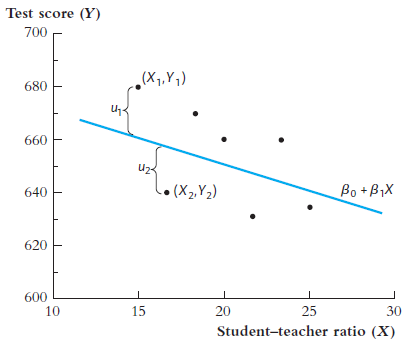
\includegraphics[scale=1.5]{diplomka obrazky/10.png}
    \caption{Znázornenie reziduí.}
    \source{Zdroj: Source of the image.}
\end{figure}

\subsection{Odhad koeficientov modelu lineárnej regresie}

Pri praktických situáciách, ako napríklad určenie dosiahnutých bodov na testoch pomocou počtu žiakov v triedach, je priesečník $\beta_0$ a sklon $\beta_1$ regresnej populačnej priamky neznámy. Teda, potrebujeme dáta, aby sme tieto neznáme koeficienty mohli odhadnúť. 

Povedzme, že chceme porovnať priemernú výšku zárobku mužov a žien, ktorí sú čerstvými absolventmi vysokej školy. Aj napriek tomu, že priemerný zárobok nami vymedzenej ženskej populácie nie je známy (nie je reálne získať dáta o zárobku každej jednej absolventky), môžeme odhadnúť priemer populácie za použitia náhodne vybranej vzorky mužov a žien, ktorí sú čerstvými absolventmi vysokej školy. Prirodzenou štatistikou pre odhad neznámej hodnoty priemerného zárobku absolventiek v populácií, bude napríklad hodnota priemerného zárobku ženských absolventiek v zozbieranej vzorke. Rovnakú logiku uplatníme pri lineárnom regresnom modeli. Nepoznáme hodnotu $\beta_{veľkosť \ triedy}$ populácie, teda sklon neznámej regresnej priamky populácie vzťahujúcej sa ku $X$ (počet žiakov v triede) a $Y$ (dosiahnuté body). Avšak, rovnako ako je možné získať informácie o priemere populácie za použitia vybranej vzorky dát z danej populácie, je taktiež možné dozvedieť sa viac o sklone populačnej regresnej priamky $\beta_{veľkosť \ triedy}$ za použitia vzorky dát. 

\subsection{Metóda najmenších štvorcov}

Model lineárnej regresie v kombinácií s metódou najmenších štvorcov spoločne tvoria jeden zo základných kameňov ekonometrie. Anglický názov predstavuje Ordinary least squares, skrátene OLS. V ďalších častiach textu budeme referovať na Metódu najmenších štvorcov pod skráteným označením OLS.

OLS vyberá koeficienty regresie tak, aby odhadnutá regresná priamka bola čo najbližšie k zozbieraným dátam. To, ako blízko je priamka k dátam, je merané súčtom štvorcov chýb, ktoré sa vyskytli pri odhadovaní $Y$ daný $X$. Teda súčet umocnenej hodnoty, ktorá sa nachádza medzi bodom na odhadnutej priamke, a reálnou nameranou hodnotou zo vzorky.  

Nech $b_0$ a $b_1$ označujú odhady $\beta_0$ a $\beta_1$. Regresná priamka založená na týchto odhadcoch je $b0 + b1X$, teda odhad $Y_i$ odhadnutý za pomoci tejto priamky je $b_0 + b_1X_i$. Chyba, ktorá sa vyskytla pri odhadovaní $í-teho$ pozorovania sa rovná $Y_i - (b_0 + b_1X_i) = Y_i - b_0 - b_1X_i$. Súčet týchto umocnených chýb naprieč všetkými $n$ pozorovaniami je:
\begin{equation}
   \sum_{i=1}^{n}(Y_i - \hat\beta_0 - \hat\beta_1{x}_i)^2 
\end{equation}

Odhad priesečníka a sklonu priamky minimalizáciou súčtu štvorcov chýb, označujeme ako Metódu najmenších štvorcov. Metóda OLS používa na značenie odhadcov $\beta_0$ a $\beta_1$ značenie $\hat\beta_0$ a $\hat\beta_1$. Takto budeme vedieť odlíšiť, či sa jedná o odhadcu, alebo parameter populácie. Teda $\hat\beta_0$ je OLS odhadca $\beta_0$ a $\hat\beta_1$ je OLS odhadca $\beta_1$. Regresná priamka OLS, taktiež nazývaná regresná priamka vzorky\footnote{SRL – Sample regression line.}, je priamka zostrojená za použitia OLS odhacov: 
\begin{equation}
   \hat\beta_0 + \hat\beta_{1}X_i.  
\end{equation}

Odhadnutá hodnota $Y_i$ dané $X_i$, odhadnutá za použitia OLS regresnej priamky, je: 
\begin{equation}
  \hat{Y}_{i} = \hat\beta_0 + \hat\beta_{1}X_i.  
\end{equation}
 
Zvyšok\footnote{Zostatok, rezíduum.} pre $í-té$ pozorovanie predstavuje rozdiel medzi $Y_i$ a jeho odhadnutou hodnotou: 
\begin{equation}
    \hat{u}_i = Y_i - \hat{Y_i}.
\end{equation}

OLS odhadcovia $\hat\beta_0$ a $\hat\beta_1$ sú vypočítaní zo vzorky, a predstavujú ekvivalent koeficientov $\beta_0$ a $\beta_1$ získaných z populácie. Takisto OLS regresná priamka, $\hat\beta_0 + \hat\beta_{1}X_i$, je vzorkovým ekvivalentom populačnej regresnej priamky, $\beta_0 + \beta_{1}X_i$. Zároveň, OLS zostatky, $\hat{u}_i$, sú vzorkovým ekvivalentom populačných náhodných zložiek, $\epsilon_i$. Mohli by sme sa pokúsiť vyrátať OLS odhadcov $\hat\beta_0$ a $\hat\beta_1$ dosadzovaním rôznych hodnôt $b_0$ a $b_1$ opakovane, až kým by sme nenašli tie, ktoré minimalizujú súčet zostatkov v uvedenom modeli. Takáto metóda by však bola veľmi vyčerpávajúca. Predstavíme si vzorce, ktoré sú vyrátané za použitia diferenciálnych a integrálnych počtov. Tieto vzorce sú používané prakticky v každom štatistickom softvéri. Vzorce si nebudeme odvodzovať. Zameriame sa na pochopenie, čo dané vzorce v skutočnosti predstavujú. 

\subsection{Meranie vhodnosti a presnosti predpovede modelu}

Po zostrojení lineárnej regresie sa naskytne otázka:“Ako dobre naša zostrojená regresná priamka vystihuje dáta?“ Je potrebné zamyslieť sa: 
\begin{enumerate}
\item Akú veľkú zásluhu na zmene závislej premennej má regresor?  
\item Sú pozorovania rozmiestnené tesne okolo regresnej priamky, alebo rozptýlené ďaleko od regresnej priamky?
\end{enumerate}
Na zodpovedanie otázok, ako dobre sedí OLS regresná priamka dátam, nám poslúži $R^2$ a štandardná chyba regresie. $R^2$ sa pohybuje v rozsahu medzi 0 a 1, a meria, aká veľká časť zmeny $Y_i$, je vysvetlená zmenou $X_i$. $R^2 = 1$ znamená, že 100\% zmeny $Y_i$ dokážeme vysvetliť pohybom $X_i$. Ak by $Y$ bola cena zmrzliny a $X$ by predstavovalo polevu alebo posýpku, ktorú si na zmrzlinu môžeme pridať, a $R^2$ by malo hodnotu 1, znamenalo by to, že pridanie polevy, ovplyvňuje 100\% zmeny v cene zmrzliny. Teda, jediný faktor ovplyvňujúci cenu zmrzliny, je poleva. Priesečník $\beta_0$ by bol 1€ (základná cena zmrzliny) a $\beta_1$ 0,3€. Pridanie jedného druhu polevy, by navýšilo cenu zmrzliny o 30centov. Každá ďalšia poleva by lineárne zvyšovala cenu o ďalších 30centov. 

Štandardná chyba regresie meria, ako poväčšine vzdialené je $Y_i$ od jej odhadnutej hodnoty, teda bodu na regresnej priamke, ktorý polohou v grafe prislúcha nameranej hodnote.  

\subsection{Koeficient determinácie - $R^2$}

$R^2$ regresie predstavuje časť rozptylu vzorky $Y$, vysvetleného, alebo odhadnutého, prostredníctvom $X$. Pomocou vzorcov na odhadnutú hodnotu $\hat{Y}_{i}$ a zostatkov $\hat{u}_{i}$, môžeme zapísať závislú premennú $Y_i$ ako súčet odhadnutej hodnoty, $\hat{Y}_{i}$, a zostatku $\hat{u}_{i}$ ako: 
\begin{equation}
   {Y}_{i} = \hat{Y}_{i} + \hat{u}_{i}.
\end{equation}
V takomto zápise predstavuje $R^2$ podiel výberového rozptylu $\hat{Y}_{i}$ ku výberovému rozptylu $Y_i$.  
Matematicky môžeme $R^2$ zapísať ako podiel vysvetleného súčtu štvorcov\footnote{SSE - Sum of Squares Explained} a celkového súčtu štvorcov\footnote{SST - Sum of squares Total}. Vysvetlený súčet štvorcov je súčet druhých mocnín odchýlok odhadovanej hodnoty, $\hat{Y}_{i}$, od jej priemeru $\overline{Y}$. Celkový súčet štvorcov je súčet druhých mocnín odchýlok $Y_i$ od jej priemeru $\overline{Y}$: 
\begin{equation}
    SSE = \sum_{i=1}^{n}(\hat{Y}_{i} - \overline{Y})^2
\end{equation}

\begin{equation}
    SST = \sum_{i=1}^{n}({Y}_{i} - \overline{Y})^2
\end{equation}

\begin{figure}[!ht]
    \centering
    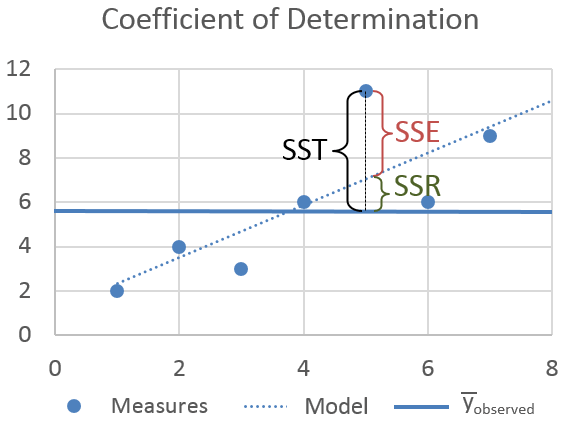
\includegraphics[scale = 0.5]{diplomka obrazky/11.png}
    \caption{Znázornenie častí $R^2$.}
    \source{Zdroj: Source of the image.}
\end{figure}
$R^2$ predstavuje pomer vysvetleného súčtu štvorcov a celkového súčtu štvorcov:
\begin{equation}
    R^2 = \frac{SSE}{SST}
\end{equation}
$R^2$ môžeme zapísať aj ako časť rozptylu $Y_i$, ktorá nie je vysvetlená $X_i$. A to súčtom štvorcov zvyškov z OLS: 
\begin{equation}
    SSR = \sum_{i=1}^{n}\hat{u}_{i}^2
\end{equation}
Z grafu vidíme, že $SST = SSR + SSE$. $R^2$ môžeme vyjadriť aj ako $1$ mínus podiel súčtu štvorcov zostatkov a celkového súčtu štvorcov: 
\begin{equation}
    R^2 = 1 - \frac{SSR}{SST}
\end{equation}
Aj keď $R^2$ vyzerá na prvý pohľad nejednoznačne na pochopenie, a rôzne umocnené súčty sa môžu mýliť, jedná sa jednoducho o korelačný koeficient $r$, umocnený na druhú mocninu. Pri regresii $Y$ na jeden regresor $X$, korelujeme premenné $X$ a $Y$. Ak $\hat\beta_1 = 0$, potom $X_i$ nevysvetľuje žiadnu zmenu $Y_i$, a odhadnutá hodnota $Y_i$ je $\hat{Y}_{i} = \hat\beta_0  = {\overline{Y}}$. V takomto prípade je vysvetlený súčet štvorcov rovný nule, a súčet štvorcov zvyškov sa rovná celkovému súčtu štvorcov, teda $R^2$ je 0. Na rozdiel, ak $X_i$ vysvetľuje všetku zmenu $Y_i$, potom $Y_i = \hat{Y}_{i}$ pre všetky $i$, a všetky zostatky sú rovné nule ($\hat{u}_{i} = 0$), teda $SSE = SST$, teda $R^2$ je v takomto prípade rovné 1. Vo všeobecnosti $R^2$ nenaberá tieto extrémne hodnoty, avšak spadá niekde medzi. $R^2$, ktoré je blízko $1$ naznačuje, že zvolený regresor je dobrý v odhadovaní $Y_i$, naopak $R^2$ blízko 0 naznačuje, že regresor nie je veľmi vhodný v odhadovaní $Y_i$. 

\subsection{Štandardná chyba regresie}

Štandardná chyba regresie\footnote{The Standard Error of the Regression} je odhadca smerodajnej odchýlky náhodnej zložky regresie $u_i$. $u_i$ a $Y_i$ sú vedené v rovnakých jednotkách, keďže $SER$ predstavuje mieru rozptylu pozorovaní okolo regresnej priamky. Napríklad, ak je závislá premenná vedená v eurách, potom $SER$ predstavuje rozsah vychýlenia od regresnej priamky, teda mieru bežnej chyby regresie, a to taktiež v eurách. Avšak náhodná zložka regresie $\epsilon_1, ..., \epsilon_n$ je nepozorovateľná, takže štandardná chyba regresie je vyrátaná za použitia ekvivalentu používaného pri práci s výberom, teda OLS zostatkami $\hat{u}_{1}, ..., \hat{u}_{n}$. Vzorec pre výpočet $SER$ je:
\begin{equation}
    SER = s_{\hat{u}} = \sqrt{s_{\hat{u}}^2}, \ kde \ s_{\hat{u}}^2 = \frac{1}{n-2}\sum_{i=1}^{n}\hat{u}_{i}^2 = \frac{SSR}{n-2},
\end{equation}
kde vzorec pre $s_{\hat{u}}^2$ pracuje s predpokladom, že výberový priemer $OLS$ zostatkov je $0$. Vzorec pre výpočet $SER$ je podobný vzorcu na výpočet výberovej smerodajnej odchýlky $Y$, s tým rozdielom, že $Y_i - \overline{Y}$ je nahradené $\hat{u}_{i}$, a menovateľ sa zmení z $n - 1$ na $n - 2$. Dôvod prečo použijeme $n - 2$ je rovnaký, ako pri použití $n - 1$. Touto úpravou menovateľa predídeme možnej odchýlke výslednej hodnoty. Odčítame $2$, pretože sme regresiou odhadovali dva koeficienty. Jedná sa o korekciu stupňov voľnosti, keďže sme odhadovali dva koeficienty, $\beta_0$  a $\beta_1$, naše dáta prišli o dva stupne voľnosti.  

Rozptyl vzorky $s^2_{Y}$ je:
\begin{equation}
    s^2_{Y} = \frac{1}{n - 1}\sum_{i=1}^{n}(Y_i - \overline{Y})^2.
\end{equation}

\newpage
\section{Testovanie hypotéz jednoduchej lineárnej regresie}

Tému si vysvetlíme na pokračovaní prípadu o počte žiakov v triede a dosiahnutom počte bodov v teste. Riaditeľ školy si nemyslí, že zmenšovanie počtov žiakov v triedach povedie k lepším výsledkom, a najímanie nových učiteľov považuje za vyhodené peniaze. Ak by sme tento výrok chceli zapísať v jazyku regresnej analýzy, uviedli by sme riaditeľove tvrdenie následovne:"Skutočný kauzálny efekt zmeny počtu žiakov v triede na dosiahnuté skóre je nulový." Teda $\beta_{veľkosť \ triedy} = 0$. 

Potrebujeme riaditeľovi vyvrátiť, že sklon priamky je nulový, čím mu dokážeme, že veľkosť triedy má vplyv na dosahované skóre žiakov. Na vyvrátenie alebo potvrdenie tejto hypotézy použijeme t – test.  

Vo všeobecnosti formulujeme t-štatistiku ako:
\begin{equation}
    t = \frac{estimátor\footnote{Estimátor = odhadca.} - predpoklad \ hypotézy}{štandardná \ chyba \ estimátora}
\end{equation}

\subsection{Obojstranný test sklonu B1}

Testovanie hypotézy o priemernej hodnote populácie za pomoci t-štatistiky:
\begin{equation}
    t = \frac{\overline{Y} - \mu_{0}}{\frac{s_{Y}}{\sqrt{n}}}
\end{equation}

Všeobecný prístup testovania hypotéz o koeficiente $\beta_1$  je rovnaký, ako pri testovaní hypotéz o priemernej hodnote populácie. Kľúčová vlastnosť testovania priemernej hodnoty populácie, na ktorú pri procedúrach spoliehame je, že pri veľkých vzorkách je výberové rozdelenie $\overline{Y}$ približne normálne.  Keďže $\beta_1$ má taktiež normálne výberové rozdelenie pri veľkých vzorkách, hypotézy o skutočnej hodnote sklonu $\beta_1$ môžeme testovať za pomoci totožnej všeobecnej metódy.  

Ako prvé potrebujeme vymedziť hypotézy, ktoré chceme testovať, teda určenie nulovej a alternatívnej hypotézy. V našom prípade je nulovou hypotézou tvrdenie riaditeľa: $\beta_{veľkosť \ triedy} = 0$. Inak povedané, pri nulovej hypotéze skutočný koeficient populácie $\beta_1$  vezme na seba určitú hodnotu, $\beta_{1,0}$\footnote{Nula znamená, že $\beta_1$ naberá hodnotu 0.}. Pri obojstrannom teste, $\beta_1$ nie je rovné $\beta_{1,0}$. Takže nulovú hypotézu a obojstrannú alternatívnu hypotézu zapíšeme ako:
\begin{equation}
    H_{0}:\beta_1 = \beta_{1,0} \ vs. \ H_{1}:\beta_{1} \neq \beta_{1,0}
\end{equation}

Pre otestovanie nulovej hypotézy $H_{0}$ postupujeme takisto, ako pri testovaní populačného priemeru. Postup si zhrnieme do troch krokov. 

\begin{enumerate}
\item Prvým krokom je vyrátanie štandardnej chyby $\hat\beta_1$, teda $SE_{\hat\beta_1}$. Štandardná chyba $\hat\beta_1$ je odhadca $\sigma_{\hat\beta_1}$, čiže smerodajnej odchýlky výberového rozdelenia $\hat\beta_1$. 
Konkrétne:
\begin{equation}
   SE(\hat\beta_{1}) = {\sqrt{\sigma^2_{\hat\beta_{1}}}},  
\end{equation}

kde:
\begin{equation}
  \hat\sigma^2_{\hat\beta_{1}} = \frac{1}{n}\times{\frac{\frac{1}{n - 2}\sum_{i=1}^{n}(X_{i}-\overline{X})^2\hat{u}_{i}^2} {\lbrack{\frac{1}{n}\sum_{i=1}^{n}(X_{i}-\overline{X})^2}\rbrack^2}} . 
\end{equation}

\item Druhým krokom je vyrátanie t-štatistiky:
\begin{equation}
    t = \frac{\hat\beta_{1} - \beta_{1,0}}{SE(\hat\beta_{1})}
\end{equation}

\item

Tretím krokom je vyrátanie $p-hodnoty$, pravdepodobnosti zaznamenania hodnoty $\hat{\beta_{1}}$, ktorá je aspoň tak odlišná od $\beta_{1,0}$, ako nami v skutočnosti vyrátaný odhad $\hat{\beta^{odhadnutá}_{1}}$, za predpokladu, že nulová hypotéza je správna. Zjednodušene povedané, sa jedná o hodnotu pravdepodobnosti, s akou nulová hypotéza $H_0$ môže nastať, respektíve, aká je pravdepodobnosť, že hodnota nulovej hypotézy nastane. Uvedené matematicky:
\begin{equation}
\begin{split}
    p-hodnota & = Pr\footnote{Pravdepodobnosť.}_{H_0}\left[|\hat\beta_{1}-\beta_{1}| > \lvert\hat\beta^{odhadnutá}_{1} - \beta_{1,0}\rvert\right] \\
   & = Pr_{H_0}\left[|\frac{\hat\beta_{1}-\beta_{1,0}}{SE(\hat\beta_{1})}| > |\frac{\hat\beta^{odhadnutá}_{1} - \beta_{1,0}}{SE(\hat\beta_{1})}| \right] \\
   & = Pr_{H_0}(|t| > |t^{odhadnutá}|),
\end{split}    
\end{equation}

\end{enumerate}

kde $Pr_{H_0}$ označuje pravdepodobnosť, vyrátanú v súlade s nulovou hypotézou. Druhá rovnosť pokračuje predelením prvej štandardnou chybou, $SE(\hat\beta_{1})$, nakoniec, $t^{odhadnutá}$ je ozajstne vyrátaná hodnota $t-štatistiky$. Keďže $\hat\beta_{1}$ je zhruba normálne rozdelené pri veľkých vzorkách, podľa nulovej hypotézy je $t-štatistika$ približne rozdelená ako štandardná normálna náhodná premenná, tak pri veľkých vzorkách platí:
\begin{equation}
    p-hodnota = Pr(|Z|>|{t^{odhadnutá}}|) = 2\Phi(-|t^{odhadnutá}|).
\end{equation}

$P-hodnota$ menšia ako $5\%$ nám poskytuje dôkaz proti nulovej hypotéze, v zmysle, že v súlade s nulovou hypotézou je pravdepodobnosť, že dostaneme hodnotu $\hat\beta_{1}$, ktorá je prinajmenšom tak vzdialená od nulovej hypotézy, ako hodnota v skutočnosti pozorovaná, menšia ako $5\%$. Ak je tomu tak, nulová hypotéza je zamietnutá na $5\%$ hladine významnosti.  

Ďalšia možnosť je otestovať hypotézu na $5\%$ hladine významnosti jednoducho, porovnaním absolútnej hodnoty $t-$ ku hodnote $1.96$, čo predstavuje kritickú hodnotu pre obojstranný test, a zamietnutie nulovej hypotézy na $5\%$ hladine významnosti, ak $|t^{odhadnutá}| > 1.96$.

\begin{figure} 
    \centering 
    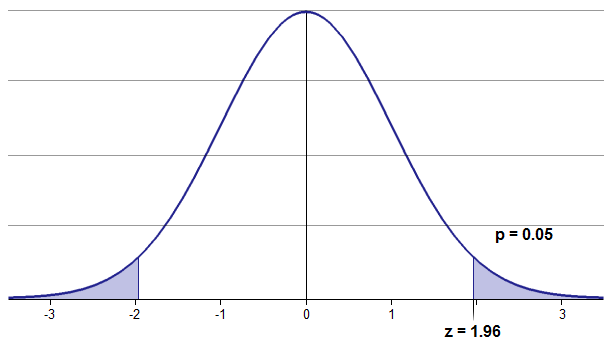
\includegraphics[scale = 0.5]{diplomka obrazky/12.png} 
    \caption{Znázornenie častí $R^2$.} 
    \source{Zdroj: }
\end{figure} 

\subsection{Jednostranné hypotézy o sklone $\beta_{1}$}

Predstavili sme si obojstranné testovanie hypotéz, kde $\beta_{1} = \beta_{1, 0}$ proti hypotéze $\beta_{1} \neq \beta_{1, 0}$. Nazýva sa to obojstranným testom hypotéz preto, pretože alternatívna hypotéza $\beta_{1}$ môže byť buď väčšia, alebo menšia ako $\beta_{1, 0}$. Niekedy sa však hodí viac použiť jednostranný test. V prípade veľkosti tried na výkon študentov si myslíme, že menšie triedy poskytnú študentom kvalitnejšie študijné prostredie, a teda lepšie výkony. V súlade s takouto hypotézou je $\beta_{1}$ negatívna. Ak si to chceme overiť, otestujeme nulovú hypotézu $\beta_{1} = 0$ (žiaden efekt) versus jednostranná alternatíva $\beta_{1} < 0$.  

Pre jednostranný test zapíšeme nulovú a alternatívnu hypotézu ako:  
\begin{equation}
    H_{0}:\beta_{1} = \beta_{1, 0} \ vs. \ \beta_{1} < \beta_{1, 0}, 
\end{equation}
   
kde $\beta_{1, 0}$ je hodnota $\beta_{1}$ podľa nulovej hypotézy (v našom prípade je to $0$, teda veľkosť triedy nemá efekt na výkon študentov), a alternatívna hypotéza $H_1$,  že $\beta_{1}$ je menej ako $\beta_{1, 0}$. Ak by sme chceli alternatívnu hypotézu obrátiť, teda, že $\beta_{1}$ je väčšie ako $\beta_{1, 0}$, nerovnicu jednoducho obrátime.  

Pretože je nulová hypotéza totožná pre jednostranný aj obojstranný test hypotéz, stavba $t-štatistiky$ je rovnaká. Jediným rozdielom medzi jedno a dvojstranným testom hypotéz, je interpretácia $t-štatistiky$. Pri jednostrannom teste je nulová hypotéza zamietnutá proti jednostrannej alternatíve pre veľké negatívne hodnoty, avšak nie pre veľké pozitívne hodnoty $t-štatistiky$. Namiesto zamietnutia pri $|t^{odhadnutá}| > 1.96$, je hypotéza zamietnutá na 5\% hladine významnosti ak $|t^{odhadnutá}| < -1.64$. $t-hodnota$ sa mení preto, pretože neodkusneme 2.5\% z každej strany, ale 5\% z jednej. Tým pádom sa zväčší chvostík rozdelenia, a zmenší sa jadro z 1.96 smerodajných odchýlok na 1.64.  

$p-hodnota$ pre jednostranný test hypotéz je získaná z kumulatívneho štandardného normálneho rozdelenia ako:
\begin{equation}
    p-hodnota = Pr(Z<t^{odhadnutá})=\Phi(t^{odhadnutá}).\footnote{Jednostranný, ľavostranný test.}
\end{equation}

Ak je alternatívnou hypotézou, že $\beta_{1}$ je väčšie ako $\beta_{1, 0}$, nerovnosť v nerovnici sa obráti, takže $p-hodnota$ je pravdepodobnosť pravého chvosta, $Pr(Z>t^{odhadnutá})$. Teda pravdepodobnosť, s akou sa hodnoty v priemere objavia v pravom chvoste rozdelenia.  

\subsection{Testovanie hypotéz o priesečníku $\beta_{0}$}

Nulová hypotéza týkajúca sa priesečníka, a jej obojstrannú alternatívnu hypotézu zapíšeme ako:
\begin{equation}
    H_{0}:\beta_{0} = \beta_{0, 0} \ vs. \ \beta_{0} < \beta_{0, 0}.
\end{equation}

Postup ostáva, ako pri testovaní sklonu. Platí to aj pri jednostrannom teste.

Testovanie hypotéz je užitočné v prípade, keď zmýšľame o konkrétnej nulovej hypotéze. Byť schopný zamietnuť, alebo nezamietnuť našu hypotézu na základe štatistickej inferencie, predstavuje silný štatistický nástroj, pri vysporiadaní sa s pochybnosťami, a pri zisťovaním informácií o populácií zo vzorky. Často sa však stáva, že žiadna konkrétna hypotéza o regresnom koeficiente nie je dominantná. V takomto prípade by sme uvítali rozmedzie hodnôt koeficientu, ktoré sú konzistentné s dátami. S týmto nám pomôžu konfidenčné intervaly (intervaly spoľahlivosti). 

\newpage
\section{Intervaly spoľahlivosti pre regresné koeficienty}

Keďže akýkoľvek štatistický odhad sklonu $\beta_{1}$, sa nevyhnutne spája s neistotou spôsobenou výberom, nemôžeme presne určiť skutočnú hodnotu $\beta_{1}$ za použitia vzorky dát. Môžeme však používať $OLS$ odhadcov, a ich štandardné chyby, na skonštruovanie intervalov spoľahlivosti pre sklon $\beta_{1}$, alebo pre priesečník $\beta_{0}$. 

\subsection{Interval spoľahlivosti pre $\beta_{1}$}

95\% konfidenčný interval pre $\beta_{1}$ má dve rovnocenné definície. Prvá tvrdí, že konfidenčný interval je súbor hodnôt, ktoré nemôžu byť zamietnuté pri použití obojstranného testu hypotéz s 5\% hladinou významnosti. Druhá tvrdí, že konfidenčný interval je interval, ktorý má 95\% pravdepodobnosť, že bude obsahovať skutočnú hodnotu $\beta_{1}$. Inak povedané, ak by sme zozbierali nekonečné množstvo vzoriek a z každej zostavili konfidenčný interval, 95\% z nich by obsahovalo skutočnú hodnotu $\beta_{1}$. Pretože tento interval obsahuje skutočnú hodnotu v 95\% všetkých vzoriek, vravíme, že máme 95\% úroveň spoľahlivosti.

Dôvod prečo sú tieto dve definície rovnocenné je nasledovný. Test hypotéz s hladinou významnosti 5\% zamietne, podľa definície, skutočnú hodnotu $\beta_{1}$ iba v 5\% prípadoch všetkých možných vzoriek. Teda v 95\% všetkých možných vzoriek skutočná hodnota nebude zamietnutá. Nakoľko 95\% interval spoľahlivosti je súborom všetkých hodnôt $\beta_{1}$, ktoré nie sú zamietnuté na 5\% hladine spoľahlivosti, skutočná hodnota $\beta_{1}$ bude obsiahnutá v intervale spoľahlivosti v 95\% všetkých možných vzoriek.

V princípe, 95\% interval spoľahlivosti môže byť vyrátaný testovaním všetkých možných hodnôt B1 (teda testovaním nulovej hypotézy $\beta_{1} = \beta_{1, 0}$ pre všetky hodnoty $\beta_{1, 0}$) na 5\% hladine spoľahlivosti za použitia t-štatistiky. 95\% konfidenčný interval je v takomto prípade súbor všetkých hodnôt $\beta_{1}$, ktoré nie sú zamietnuté. Zostrojenie t-štatistiky pre všetky hodnoty $\beta_{1}$ by však zabralo nekonečne veľa času. 
Jednoduchší spôsob zostrojenia intervalu spoľahlivosti sa naskytne, keď si uvedomíme, že t-štatistika odmietne vyslovenú hodnotu hypotézu $\beta_{1, 0}$ v prípade, keď je $\beta_{1, 0}$ mimo intervalu $\hat\beta_{1} \pm 1.96SE(\hat\beta_{1})$. To znamená, že 95\% konfidenčný interval pre $\hat\beta_{1}$ je interval: 
\begin{equation}
    [\hat\beta_{1} - 1.96SE(\hat\beta_{1}) \ , \ \hat\beta_{1} + 1.96SE(\hat\beta_{1})].
\end{equation}

\subsection{Interval spoľahlivosti pre $\beta_0$}

95\% konfidenčný interval pre $\beta_0$ zostrojíme rovnako ako pri $\beta_1$. Namiesto $\hat\beta_1$  použijeme $\hat\beta_0$  a namiesto $SE(\hat\beta_{1})$ zas $SE(\hat\beta_{0})$.

$OLS$ regresia výšky dosiahnutého hodnotenia na veľkosť tried poskytla hodnoty odhadcov $\hat\beta_{1} = -2.28$ a $SE(\hat\beta_{1}) = 0.52$. Obojstranný 95\% interval spoľahlivosti pre $\hat\beta_{1}$ je $\{-2.28 \pm 1.96 \times 0.52\}$, alebo $\{-3.30 \leq \beta_{1} \leq -1.26\}$. Hodnota $\beta_{1} = 0$ nie je obsiahnutá v intervale spoľahlivosti, takže nulová hypotéza $\beta_{1} = 0$ môže byť zamietnutá na hladine spoľahlivosti 5\%. 

\subsection{Interval spoľahlivosti pre predpovedaný efekt zmeny $X$}

Konfidenčný interval pre $\beta_1$ môže byť použitý na zostrojenie 95\% intervalu spoľahlivosti pre predpovedaný efektu všeobecnej zmeny v $X$. Uvažujme so zmenou $X$ v určitej miere $\Delta x$. Očakávaná zmena v $Y$ spojená so zmenou v $X$ je $\beta_{1} \Delta x$. Sklon populácie $\beta_1$ nie je známy, avšak keďže môžeme skonštruovať konfidenčný interval pre $\beta_1$, môžeme taktiež zostrojiť konfidenčný interval pre očakávaný efekt $\beta_{1} \Delta x$. Nakoľko jeden koniec 95 intervalu spoľahlivosti pre $\beta_1$ je $\hat\beta_{1} - 1.96SE(\hat\beta_{1})$, a predpovedaný následok zmeny $\Delta x$ za použitia odhadu pre $\beta_1$ je $[\hat\beta_{1} - 1.96SE(\hat\beta_{1})] \times \Delta x$. Druhý koniec intervalu spoľahlivosti je $\hat\beta_{1} + 1.96SE(\hat\beta_{1})$, a predpovedaný efekt zmeny za použitia odhadu je $[\hat\beta_{1} + 1.96SE(\hat\beta_{1})] \times \Delta x$. Teda 95\% interval spoľahlivosti pre dôsledok zmeny $X$ v miere $\Delta x$ môžeme vyjadriť ako 95\% konfidenčný interval pre $\beta_{1} \Delta x$:
\begin{equation}
   [\hat\beta_{1} - 1.96SE(\hat\beta_{1})\Delta x \ , \ \hat\beta_{1} + 1.96SE(\hat\beta_{1})\Delta x]. 
\end{equation}
Uveďme si príklad. Ak by sme chceli zmeniť pomer študentov k učiteľom (vyjadrenie veľkosti tried) o 2 jednotky, tak keďže $95\%$ interval spoľahlivosti pre $\beta_1$ je $[-3.30, -1.26]$, dôsledok zníženia pomeru o 2 jednotky by mohol mať dopad až $-3.30 \times (-2) = 6.6$ bodu, alebo len $-1.26 \times (-2) = 2.52$. Takže zníženie pomeru študentov k učiteľom o hodnotu 2 by malo odhadovaný efekt navýšenia bodovej úspešnosti študentov v testoch medzi 2.52 a 6.6 bodov, s 95\% úrovňou spoľahlivosti. Ak je pomer študentov k učiteľom $10:1$, tak na jedného učiteľa pripadá $10$ žiakov. Zníženie z 10 na 8 študentov na jedného učiteľa by malo predpovedaný efekt vyrátaný vyššie. 

\newpage
\section{Heteroskedasticita a Homoskedasticita}

Náhodná zložka ${u}_{i}$  je homoskedastická, ak rozptyl podmieneného rozdelenia ${u}_{i}$ daný\footnote{(${u}_{i}$ | $X_{i}$)} $X_{i}$, je konštantný pre $i = 1, ..., n$, a obzvlášť nezávisí na $X_{i}$. Ak táto podmienka nie je splnená, hovoríme, že náhodná zložka je heteroskedastická. Najlepšie to vysvetlíme ilustráciou náhodných zložiek a porovnaním ich rozptylov vizuálne. Distribúcia náhodnej zložky ${u}_{i}$ je ilustrovaná pre viaceré hodnoty $x$. Keďže sa toto rozdelenie týka konkrétne vyznačených hodnôt $x$, jedná sa o podmienené rozdelenie ${u}_{i}$ daný $X_{i} = x$, ktoré má podľa prvej podmienky najmenších štvorcov priemer rovný nule pre všetky $x$. Na prvom grafe majú všetky tieto podmienené rozdelenia rovnaký rozptyl, inak povedané, rozptyl všetkých týchto rozdelení je rovnaký pre rôzne hodnoty $x$. Podmienená zmena ${u}_{i}$ daný $X_{i} = x$, nezávisí od $x$, teda neznáme zložky sú homoskedastické. 

Na druhej strane, druhý graf zobrazuje prípad, kedy sa podmienené rozdelenie ${u}_{i}$ rozpína s narastajúcim $x$. Pri malých hodnotách $x$ je rozdelenie úzke, avšak pri väčších hodnotách $x$ je rozdelenie širšie. V druhom grafe rozptyl ${u}_{i}$ daný $X_{i} = x$ narastá s $x$, teda neznáma zložka je heteroskedastická. 
\begin{figure}[!ht] 
    \centering 
    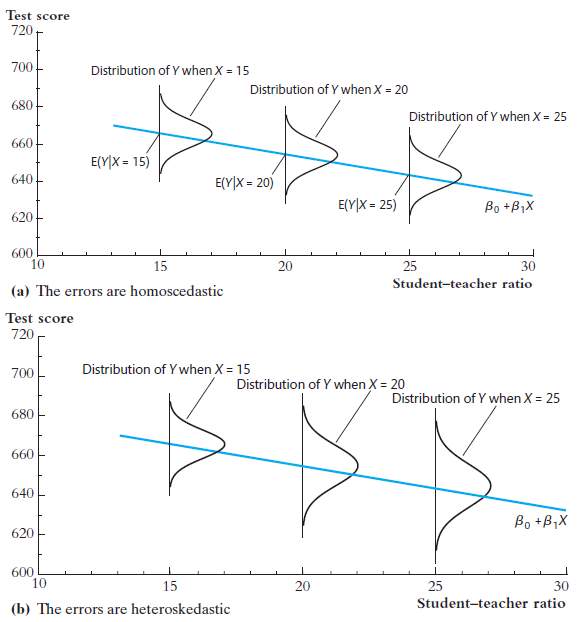
\includegraphics[scale = 1.25]{diplomka obrazky/13.png} 
    \caption{a) Homoskedasticita. b) Heteroskedasticita.} 
    \source{Zdroj: Source of the image.} 
\end{figure} 

Pretože metóda najmenších štvorcov nemá medzi svojimi predpokladmi žiadne vymedzené obmedzenia týkajúce sa podmieneného rozptylu, predpoklad platí aj v prípade homoskedasticity aj heteroskedasticity. Z toho dôvodu $OLS$ odhadcovia ostanú nestranní, konzistentní a asymptoticky normálni, či už je neznáma zložka heteroskedastická, alebo homoskedastická. Existujú vzorce na výpočet odchýlky, ktoré vopred rátajú, že neznáma zložka je homoskedastická. Z historických dôvodov sú často vzorce tohto typu prednastavené v štatistickom softvéri. Ak je náhodná zložka heteroskedastická, tieto vzorce nie je vhodné použiť. Napríklad, vyrátaná t-štatistika nebude mať štandardné normálne rozdelenie, ani pri veľkých vzorkách. Na druhú stranu, keďže homoskedasticita je mimoriadny prípad heteroskedasticity, odhadcovia $\hat\sigma^2_{\hat\beta_{1}}$ a $\hat\sigma^2_{\hat\beta_{0}}$ rozptylu $\hat\beta_{1}$ a $\hat\beta_{0}$ ponúknu platný štatistický úsudok, či už je neznáma zložka heteroskedastická, alebo homoskedastická. Tým pádom sú testy hypotéz a intervaly spoľahlivosti založené na týchto štandardných chybách platné, či už sú náhodné zložky heteroskedastické, alebo nie. Takéto štandardné chyby sa nazývajú heteroskedasticky-robustné. Ak sú štandardné chyby za použitia vzorcov aj pre homoskedasticitu aj heteroskedastickú robustnosť rovnaké, nič sa nestane, ak použijeme heteroskedasticky-robustné štandardné chyby. Ak sa líšia, mali by sme použiť výsledok z heteroskedasticky-robustného výpočtu. Najjednoduchší spôsob je takéto heteroskedasticky-robustné vzorce pre výpočet štandardnej chyby používať stále. 

\newpage
\section{Viacnásobná lineárna regresia}

Aj napriek tomu, že školy s menším podielom študentov k učiteľom majú tendenciu mať lepšie výsledky v testoch, skutočnosť je pravdepodobne taká, že okrem počtu žiakov v triedach vplýva na výšku dosiahnutých bodov aj niečo iné. Cieľom viacnásobnej lineárnej regresie, je práve vyhnutie sa odchýlke, ktorá môže byť spôsobená vynechaním vplyvných faktorov, ich  nezakomponovaním do lineárnej regresie. Vynechané premenné, ako napríklad vlastnosti študentov, môžu spôsobiť, že $OLS$ odhadca odhadne skreslené hodnoty koeficientov, teda $OLS$ odhadca bude neobjektívny, skreslený. Hlavnou myšlienkou viacnásobnej lineárnej regresie je, že ak máme dáta o týchto vynechaných premenných, môžeme ich zahrnúť do lineárnej regresie ako ďalší regresor, a takto odhadnúť kauzálny efekt jedného regresora (pomer študentov k učiteľom) , zatiaľ čo ostatné premenné zachováme konštantné (vlastnosti študentov). 

Alternatívne, ak nás viac zaujíma predikcia než kauzálna inferencia, model viacnásobnej regresie nám umožňuje použiť viacero premenných ako regresory, t.j. viacero prediktorov, na vylepšenie predikcií vytvorených jedným regresorom jednoduchou lineárnou regresiou.

\subsection{Odchýlka spôsobená vynechanou premennou}

Ak je regresor (pomer študentov k učiteľom) korelovaný s nezávislou premennou (vlastnosti študentov), ktorú sme do modelu nezahrnuli, avšak ovplyvňuje závislú premennú modelu, bude $OLS$ odhadca trpieť odchýlkou vynechanej premennej. 
Odchýlka vynechanej premennej nastane, ak sú splnené dve podmienky:
\begin{enumerate}
\item opomenutá premenná je korelovaná s regresorom (nezávislou premennou), ktorý je zahrnutý v modeli,
\item opomenutá premenná má súvis a vplyv na závislú premenú.
\end{enumerate}
Platnosť podmienok si osvetlíme na nasledujúcich príkladoch:
\begin{enumerate}
\item Za vynechanú premennú považujeme vlastnosť študentov, konkrétne ich jazykové znalosti, merané tým, či školy do ktorých chodia, vyučujú v ich materinskom jazyku, alebo nie. Jazykové znalosti, a pomer študentov k učiteľom sú korelované (školy pre prisťahované deti zvyknú mať väčší počet detí na jedného učiteľa). Tým je prvá podmienka odchýlky vynechanej premennej splnená. Je pochopiteľné, že študenti, ktorí v jazyku používanom na škole nie sú na úrovni domácich, budú mať ťažšie podmienky pri písaní testov, a teda očakávame aj horšie výsledky. Čím spĺňame aj druhú podmienku. Takto by sme teda vynechaním tejto premennej v modeli zapríčinili, že by $OLS$ odhadca nesprávne premietol dáta do koeficientov odhadcov.
\item Ďalšou vynechanou premennou je čas dňa, kedy študenti tento štandardizovaný test, na ktorom je postavený náš súbor dát, písali. Ak sa čas písania testu líši medzi rôznymi mestskými časťami kvôli dôvodu, ktorý nie je spojený s počtom žiakov v triede, potom prvá podmienka nie je splnená. Avšak čas písania testu môže ovplyvňovať výšku dosiahnutého hodnotenia v teste (bdelosť študentov nie je počas celého dňa rovnaká), tým pádom, premenná spĺňa druhú podmienku. Nuž, keďže v tomto prípade čas písania testu nie je korelovaný s počtom žiakov na učiteľa, táto premenná (pomer študentov k učiteľom) nemôže chybne zachytiť efekt vynechanej premennej (fáza dňa, kedy bol test absolvovaný), na zmenu závislej premennej (dosiahnuté skóre). Čo znamená, že nezahrnutie premennej o fáze dňa, kedy bol test písaný, nebude mať za následok odchýlku vynechanej premennej. 
\item Ďalšia vynechaná premenná predstavuje počet parkovacích miest pre učiteľov na študenta. Táto premenná spĺňa prvú podmienku, ale druhú nie. Školy s viacerými učiteľmi na žiaka, majú pravdepodobne viac parkovacích miest pre učiteľov, čo zaručuje splnenie prvej podmienky. Avšak, vyučovanie prebieha vo vnútorných priestoroch školy, a nie na parkovisku. Čiže parkovacie miesta nemajú žiaden priamy efekt na vyučovanie, čo odporuje splneniu druhej podmienky. Pretože parkovacie miesta na žiaka nemajú vplyv na výšku skóre, vynechanie tejto premennej z modelu nepovedie k odchýlke vynechanej premennej.
\end{enumerate}

Prítomnosť odchýlky opomenutej premennej znamená, že predpoklad najmenších štvorcov pre kauzálnu inferenciu $E(u_{i} | X_{i}) = 0$, nie je splnený. Aby sme pochopili prečo, pripomeňme si, že náhodná zložka $u_i$ v modeli jednoduchej lineárnej regresie reprezentuje všetky faktory, iné ako $X_{i}$, ktoré majú vplyv na $Y_{i}$. Ak nejaký z týchto iných faktorov je korelovaný s $X_{i}$, znamená to, že náhodná zložka (ktorá obsahuje tento faktor) je korelovaná s $X_{i}$. Inak povedané, ak má opomenutá premenná vplyv na $Y_{i}$, tento vplyv je zahrnutý v náhodnej zložke, a ak je táto opomenutá premenná korelovaná s $X_{i}$, potom je náhodná zložka korelovaná s $X_{i}$. Pretože $u_{i}$ a $X_{i}$ sú korelované, podmienený priemer (očakávaná hodnota) $u_{i}$ daný $X_{i}$ je nenulový. Táto korelácia porušuje prvú podmienku metódy najmenších štvorcov, čoho dôsledkom je odchýlka $OLS$ odhadcu. Táto odchýlka nezmizne ani pri veľkých vzorkách, čo robí $OLS$ odhadcu nekonzistentným. 

\subsubsection{Vzorec pre odchýlku vynechanej premennej}

Označme koreláciu medzi $X_{i}$ a $u_{i}$ ako $corr(X_{i}, u_{i}) = \rho_{Xu}$. Predpokladajme, že druhá a tretia podmienka najmenších štvorcov platí, avšak prvá nie, pretože $\rho_{Xu}$ je nenulové. $OLS$ odhadca má limitu:
\begin{equation}
    \hat\beta_{1}\xrightarrow[\text{}]{\text{\; p \; }}\beta_{1}+\rho_{Xu}\frac{\sigma_{u}}{\sigma_{X}}.
\end{equation}

Ak veľkosť vzorky rastie, $\hat\beta_{1}$ je bližšie k $\beta_{1} + \rho_{Xu}(\sigma_{u} / \sigma_{X})$ s narastajúcou pravdepodobnosťou. 
\begin{enumerate}
\item  Odchýlka opomenutej premennej je problém, či už je vzorka malá alebo veľká, pretože $\hat\beta_{1}$  nekonverguje s pravdepodobnosťou k skutočnej hodnote $\beta_{1}$. $\hat\beta_{1}$ má odchýlku, a je nekonzistentný, čo znamená, že $\hat\beta_{1}$ je nekonzistentným odhadcom $\beta_{1}$, za prítomnosti odchýlky opomenutej premennej. Časť vzorca $\rho_{Xu}(\sigma_{u} / \sigma_{X})$ predstavuje odchýlku v $\hat\beta_{1}$, ktorá pretrvá aj pri veľkých vzorkách.  
\item Veľkosť odchýlky závisí od absolútnej výšky korelácie regresora, a náhodnej zložky. 
\item Smer odchýlky závisí na $pozitivite / negativite$ korelácie medzi $X$ a $u$.
\end{enumerate}
Náhodné kontrolované experimenty\footnote{RCT - Randomized contorlled trials.} napomáhajú odstraňovaniu veľkého množstva týchto odchýlok.

\subsection{Model viacnásobnej lineárnej regresie}

Model viacnásobnej lineárnej regresie rozširuje model jednoduchej lineárnej regresie o dodatočné regresory. Pri použití modelu pre kauzálnu inferenciu nám model s viacerými regresormi umožňuje odhadnúť efekt na $Y_{i}$ pri úprave jednej premennej ($X_{1i}$), pričom ostatné premenné ($X_{2i}$, $X_{3i}$, atď) ostanú konštantné. Pri príklade o výške dosiahnutých bodov študentov a počtu učiteľov na žiaka nám umožní model viacnásobnej lineárnej regresie izolovať efekt počtu učiteľov na žiaka ($X_{1i}$) na výšku skóre ($Y_{i}$), pričom premenná $X_{2i}$, ktorá znázorňuje pomer žiakov, ktorí neštudujú v materinskom jazyku, ostane napriek zmene (v $X_{1i}$) konštantná. Pri použití modelu pre predikciu, použitie viacerých regresorov môže vylepšiť predikcie. 

\subsubsection{Regresná priamka populácie}

Uvažujme s dvoma nezávislými premennými $X_{1i}$ a $X_{2i}$. V modeli viacnásobnej lineárnej regresie je priemerný vzťah medzi týmito dvoma nezávislými premennými a závislou premennou $Y$ vyjadrený lineárnou funkciou:
\begin{equation}
    E(Y_{i} | X_{1i} = x_{1},X_{2i}=x_{2}) = \beta_{0} + \beta_{1}x_{1} + \beta_{2}x_{2},
\end{equation}
kde $E(Y_{i} \ daný \ X_{1i} = x_{1},X_{2i}=x_{2})$ je podmienená očakávaná hodnota $Yi$ daný, že $X_{1i} = x_{1},X_{2i}=x_{2}$. 
Takáto lineárna funkcia sa v modeli viacnásobnej lineárnej regresie nazýva populačná regresná priamka, alebo populačná regresná funkcia. Je to vzťah, ktorý priemerne platí v populácií pre $Y$ a všetky regresory $X_k$. Koeficient $\beta_{0}$ je priesečník, koeficient $\beta_{1}$ je koeficient sklonu $X_{1i}$ a koeficient $\beta_{2}$ je koeficient sklonu $X_{2i}$. Interpretácia koeficientu $\beta_{1}$ v modeli viacnásobnej lineárnej regresie populácie sa líši od jednoduchej lineárnej regresie, kde $X_{1i}$ bol jediným regresorom. V uvedenom modeli je $\beta_{1}$ odhadnutá zmena $Y$ medzi dvoma pozorovaniami, pri zmene $X_1$ o jednu jednotku, pričom $X_2$ ostáva konštantné. Táto interpretácia $\beta_{1}$ vyplýva z porovnávania odhadov dvoch pozorovaní s rovnakou hodnotou $X_2$, avšak dvoma hodnotami $X_1$, ktoré sa líšia o $\Delta X_{1}$. Tým pádom prvé pozorovanie pracuje s hodnotami $X$ ($X1$ a $X2$), a druhé pozorovanie s hodnotami $X$ ($X_{1} + \Delta X_{1}, X_{2}$). Odhadovaná hodnota $Y$ pre prvé pozorovanie je daná rovnicou:
\begin{equation}
    Y = \beta_{0} + \beta_{1} X_{1} + \beta_{2} X_{2}.
\end{equation}

Odhadovaná hodnota $Y$ pre druhé pozorovanie je $Y + \Delta Y$, pre ktorú:
\begin{equation}
    Y + \Delta Y = \beta_{0} + \beta_{1} (X_{1} + \Delta X_{1}) + \beta_{2} X_{2}.
\end{equation}
Rovnicu pre $\Delta Y$ pokiaľ ide o $\Delta X_{1}$ dostaneme odčítaním rovnice $Y = \beta_{0} + \beta_{1} X_{1} + \beta_{2} X_{2}$ od $Y + \Delta Y = \beta_{0} + \beta_{1} (X_{1} + \Delta X_{1}) + \beta_{2} X_{2}$, výsledkom čoho je $\Delta Y = \beta_{1}\Delta X_{1}$, čo môžeme prepísať ako:
\begin{equation}
    \beta_{1} = \frac{\Delta Y}{\Delta X_{1}},
\end{equation}
pričom udržiavame $X_2$ konštantné.

Koeficient $\beta_{1}$ je teda rozdiel v odhadnutej hodnote $Y$ (rozdiel podmienených očakávaní $Y$) medzi dvomi pozorovaniami pri jednotkovej zmene v $X_1$, pričom držíme $X_2$ konštantné. $\beta_{1}$ predstavuje čiastkový efekt $X$ na $Y$, držiac $\beta_{1}$ nemenné. Interpretácia $\beta_{0}$ je rovnaká ako pre jednoduchú lineárnu regresiu.  
Všeobecný model pre viacnásobnú regresiu je:
\begin{equation}
    Y_{i} = \beta_{0} + \beta_{1} X_{1i} + \beta_{1} X_{2i} + ... + \beta_{k} X_{ki} + \epsilon_{i}, \ i = 1, ..., n,
\end{equation}
kde:
\begin{itemize}
\item  $Y_i$ je $í-te$ pozorovanie závislej premennej $X_{1i}, X_{2i}, ..., X_{ki}$ sú $í-te$ pozorovania každého z $k$ regresorov, a $\epsilon_i$ je náhodná zložka.
\item Názvoslovie $OLS$ pre viacnásobný model lineárnej regresie je rovnaké ako pre model jednoduchej lineárnej regresie. 
\end{itemize}

Definícia homoskedasticity a heteroskedasticity v modeli viacnásobnej regresie je obšírnejšia v porovnaní s definíciou pre model jednoduchej regresie. Náhodná zložka $\epsilon_{i}$ v modeli viacnásobnej regresie je homoskedastická, ak rozptyl podmieneného rozdelenia $\epsilon_{i}$ daný $X_{1i}, ..., X_{ki}, var(u_{i}|X_{1i}, ..., X_{ki})$, je konštantný pre $i = 1, ..., n$, čím nie je závislý na hodnotách $X_{1i}, ..., X_{ki}$. Ak táto podmienka nie je splnená, náhodná zložka je heteroskedastická.

\subsection{Meranie vhodnosti modelu vo viacnásobnej regresii}

\subsubsection{Štandardná chyba regresie}

Vo viacnásobnej regresii je štandardná chyba regresie vyrátaná ako:
\begin{equation}
    SER = s_{\hat{u}} = \sqrt{s_{\hat{u}}^2},  \ kde \  s_{\hat{u}}^2 =\frac{1}{n-k-1}\sum_{i=1}^{n}\hat{u_{i}}^2 = \frac{SSR}{n-k-1}.
\end{equation}

Jediným rozdielom medzi definíciou štandardnej chyby regresie vo viacnásobnej a jednoduchej regresii je iný menovateľ. V definícií pre viacnásobnú regresiu je to $n - k - 1$, namiesto $n - 2$. Menovateľ $n - 2$ pri regrersii s jedným regresorom upravuje odhadcu kvôli nadol smerujúcej odchýlke, ktorá vzniká pri odhade dvoch koeficientov, priesečníku a sklonu. Vo vzorci pre viacnásobnú regresiu menovateľ $n - k - 1$ upravuje pre nadol smerujúcu odchýlku, ktorá vzniká pri odhade $k + 1$ koeficientov. Takisto ako pri už skôr uvedenom vzorci pre jednoduchú regresiu, použitie $n - k - 1$ namiesto $n$ sa nazýva úprava stupňov voľnosti. Pri jednom regresore sa $k = 1$, teda vzorec pre odhad štandardnej chyby regresie pre jednoduchú a viacnásobnú regresiu bude zhodný. Pri veľkom $n$ je efekt úpravy stupňov voľnosti zanedbateľný.   

\subsubsection{Koeficient determinácie - $R^2$}

Pri viacnásobnej regresii vzrastie $R^2$ pri každom pridaní nového regresora, s výnimkou regresora, ktorého odhadnutý koeficient je presne 0. Pri použití $OLS$ metódy na odhad modelu s dvoma regresormi, $OLS$ nájde hodnotu koeficientov, ktorá je najmenšou pri súčte štvorcov zvyškov regresie\footnote{SSR.}. Ak $OLS$ vyhodnotí hodnotu koeficientu odhadcu ako 0, potom ostane súčet štvorcov zvyškov v modeli nezmenený bez ohľadu na to, či pridaná premenná v modeli bude, alebo nebude zahrnutá. Ak však $OLS$ vyhodnotí hodnotu koeficientu odhadcu inú ako presne 0, znamená to, že táto hodnota koeficientu znížila súčet štvorcov zvyškov v regresii v pomere k modelu, ktorý túto premennú nezahŕňa. V praxi je veľmi nezvyčajné pre odhadovaný koeficient, aby mal hodnotu 0, takže vo všeobecnosti každá pridaná premenná znižuje súčet štvorcov zvyškov regresie. To však znamená, že $R^2$ vo všeobecnosti vzrastie (a nikdy neklesne) pri každom pridaní nového regresora. 

\subsubsection{Upravený koeficient determinácie - $R^2$}

Pretože $R^2$ vzrastie pri každom pridaní novej premennej, nárast koeficientu $R^2$ neznamená, že pridaná premenná v skutočnosti vylepšila vhodnosť modelu. $R^2$ nám potom poskytne premrštený odhad toho, ako dobre pasuje regresia dátam. 
Upravený koeficient determinácie $R^2$, alebo $\overline{R^2}$, je upravená verzia $R^2$, ktorá nemusí v každom prípade vzrásť, po pridaní novej premennej do modelu. $\overline{R^2}$ vyjadríme ako:
\begin{equation}
    \overline{R^2} = 1 - \frac{n - 1}{n - k - 1} \frac{SSR}{TSS} = 1 - \frac{s_{\hat{u}}^2}{s_{Y^2}}.
\end{equation}

Rozdiel medzi rovnicou 8.8\footnote{Upravený koeficient determinácie.} a 8.9\footnote{Koeficient determinácie.} je, že pomer súčtu štvorcov zvyškov k celkovému súčtu štvorcov je vynásobený činiteľmi $(n - 1)$ v čitateli, a $(n - k - 1)$ v menovateli.
\begin{equation}
     R^2 = 1 - \frac{SSR}{SST}.
\end{equation}
Druhý výraz v rovnici 8.8 vyjadruje, že upravený koeficient determinácie je 1 mínus pomer výberového rozptylu zvyškov $OLS$ (s úpravou stupňov voľnosti) k výberovému rozptylu $Y$. 

Pre upravený koeficient determinácie platia tri zaujímavosti:
\begin{enumerate}
    \item $(n - 1) / (n - k - 1)$ je stále väčšie ako 1, takže $\overline{R^2}$ je stále menšie ako $R^2$.
    \item Pridanie regresora má dva opačné efekty na $\overline{R^2}$. Na jednej strane sa zníži $SSR$, čo zvýši $\overline{R^2}$, na druhej strane však narastie $(n - 1) / (n - k - 1)$, čo $\overline{R^2}$ zníži. Či v konečnom dôsledku $\overline{R^2}$ narastie, alebo poklesne, závisí od toho, ktorý z týchto dvoch javov bude silnejší.
    \item $\overline{R^2}$ môže byť záporný. Jav nastane, ak všetky regresory spoločne znížia súčet štvorcov zvyškov v tak malom množstve, že nedokážu vykompenzovať efekt $(n - 1) / (n - k - 1)$.    
\end{enumerate}

\newpage
\section{Multikolinearita}

Jednou z podmienok pre správne fungovanie $OLS$ je neprítomnosť dokonalej multikolinearity v modeli. Multikolinearita môže byť dokonalá alebo nedokonalá. Regresory sú vystavené dokonalej multikolinearite, respektíve sú dokonalo multikolineárne, ak jeden z regresorov existuje ako dokonalá lineárna funkcia iného regresora. 

Je dôležité rozumieť, prečo dokonalá multikolinearita predstavuje problém pre výpočet $OLS$. Našťastie to môžeme veľmi jednoducho vysvetliť príkladom. Povedzme, že chceme odhadnúť koeficient odhadcu $STR$\footnote{Student-teacher-ratio (pomer žiakov k učiteľom).} v regresii, kde regresujeme výkonnosť v testoch na $STR_i$ a $PctELi$\footnote{Percentage of english learners (percento žiakov, kt. sa učia v cudzom jazyku).}, avšak namiesto $PctELi$ napíšeme druhýkrát $STR_i$, takže regresujeme výkonnosť v testoch na $STR_i$ a $STR_i$. Toto je perfektný príklad dokonalej multikolinearity, keďže jeden regresor ($STR$) je dokonalou lineárnou funkciou iného regresora (v našom prípade to je opakovaný výskyt $STR$). Zvyčajne je prístup k odhaleniu multikolinearity ošetrený štatistickým softvérom. Buď sám odstráni výskyt jednej z multikolineárnych premenných, alebo odmietne vyrátať $OLS$, a vyhodí nám chybu. Matematickým odôvodnením tohto zlyhania je, že pri multikolinearite regresorov nútime $OLS$ metódu deliť nulou. 

Ak sa nad multikolineritou zamyslíme čisto intuitívne, dokonalá multikolinearita predstavuje problém, lebo od regresie požadujeme odpoveď na nelogické otázky. Vo viacnásobnej regresii predstavuje koeficient regresora efekt zmeny tohto regresora, pričom ostatné regresory držíme nemenné. Napríklad $0.34 \times STR$ predstavuje pozitívnu zmenu regresanta, efekt, o koeficient $0.34$, pri zmene $STR$ o jednu jednotku. Pri našej hypotetickej regresií výšky dosiahnutého skóre na $STR$ a $STR$, koeficient prvého $STR$ predstavuje efekt na výšku dosiahnutého skóre pri zmene prvého $STR$, pričom držíme druhé $STR$ nemenné. Toto nedáva zmysel, keďže sa jedná o rovnaké súbory dát, a rovnaké regresory, teda $OLS$ nemôže odhadnúť tento nezmyselný čiastkový efekt na výšku skóre. 

Riešením dokonalej multikolinearity v našej hypotetickej regresií by bolo jednoduché opravenie pravopisnej chyby, a nahradenie nesprávneho regresora tým správnym, zaumieneným. Pri výskyte dokonalej multikolinearity sa často jedná o logickú chybu pri výbere regresora, alebo nepovšimnutie si istých súvislostí, ktoré boli skryté v dátach. Všeobecným riešením dokonalej multikolinearity je modifikácia regresorov, a korektná špecifikácia modelu. 

\subsection{Nedokonalá multikolinearita}

Napriek podobným názvom je nedokonalá multikolinearita koncepčne dosť odlišná od dokonalej multikolinearity. Nedokonalá multikolinearita znamená, že dva alebo viac regresorov je vysoko korelovaných v zmysle, že existuje lineárna funkcia regresora, ktorá je vysoko korelovaná s iným regresorom. Nedokonalá multikolinearita nepredstavuje teoreticky žiaden problém pre $OL$S odhadcov, práve naopak, jedným z použití $OLS$ metódy je aj vytriedenie nezávislých vplyvov rozličných regresorov, keď sú regresory korelované. 

Ak sú regresory nedokonalo korelované, koeficient aspoň na jednom z jednotlivých regresorov bude odhadnutý nepresne. Ako príklad si uveďme regresiu výšky dosiahnutého skóre v testoch na $STR$ a $PctEL$. Povedzme, že by sme pridali tretí regresor, a to percento rezidentov v mestskej časti, ktorí sú imigranti, teda majú iný materinský jazyk ako krajina, do ktorej sa prisťahovali. Keďže sa prisťahovali a chcú sa naučiť jazyk krajiny, táto tretia premenná bude vysoko korelovaná s premenou $PctEL$. Kvôli vysokej korelácií týchto dvoch regresorov by bolo obtiažne odhadnúť koeficient pre $PctEL$, za držania podielu imigrantov nemenným. Inými slovami, súbor dát s ktorým pracujeme by nám poskytol veľmi málo informácií ohľadom toho, čo sa stane s výškou skóre, ak by bolo $PctEL$ nízke, avšak podiel prisťahovalcov vysoký, a naopak. Keďže percento žiakov, ktorí sa učia jazyk by bolo nízke, avšak percento imigrantov vysoké, očakávali by sme, že percento žiakov, ktorí sa učia jazyk by malo byť vyššie, teda predpokladali by sme skreslenie dát alebo veľký rozptyl. V našom prípade by výsledkom bol jednoducho vyšší rozptyl koeficientu odhadcu $PctEL$, v porovnaní ak by $PctEL$ a percento prisťahovalcov neboli korelované. 

Efekt nedokonalej multikolinearity na rozptyl $OLS$ odhadcov si môžeme ukázať matematicky preskúmaním rovnice rozptylu $\hat\beta_{1}$ pre viacnásobnú regresiu s dvoma regresormi ($X_1$ a $X_2$), a pre špeciálny prípad homoskedastickej náhodnej zložky.
\begin{equation}
    \sigma_{\hat\beta_{1}}^2 = \frac{1}{n}\left(\frac{1}{1-\rho_{X_{1}, X_{2}}^2}\right)\frac{\sigma_{u}^2}{\sigma_{X_{1}}^2}.
\end{equation}

Rozptyl $\hat\beta_{1}$ je nepriamo úmerný k $1-\rho_{X_{1}, X_{2}}^2$, kde $\rho_{X_{1}, X_{2}}^2$ predstavuje koreláciu medzi $X_1$ a $X_2$. Čím väčšia je korelácia medzi týmito dvoma regresormi, tým bližšie je výraz k nule, čo v konečnom dôsledku zväčšuje rozptyl $\hat\beta_{1}$. Vo všeobecnosti platí, že ak je viacero regresorov nedokonalo multikolineárnych, koeficient aspoň jedného z nich bude nepresne odhadnutý. Budú mať teda veľký výberový rozptyl. 

Dokonalá multikolinearita je problém, ktorý často signalizuje prítomnosť logickej chyby. Na rozdiel od nedokonalej multikolinearity, ktorá by sa skôr ako chybou dala nazvať vlastnosťou, či charakteristickým znakom $OLS$, dát a otázky, ktorú sa snažíme zodpovedať. Ak do modelu zahrnieme všetky premenné, ktoré sme tam chceli uviesť, potom nedokonalá multikolinearita naznačuje, že bude náročné presne odhadnúť jeden alebo viacero čiastkových efektov za použitia dát, ktoré máme práve po ruke.  

\newpage
\section{Testovanie hypotéz viacnásobnej lineárnej regresie}

Koncepčne sa k výpočtu štandardnej chyby viacnásobnej regresie staviame rovnako ako v prípade jednoduchej regresie. Kľúčové myšlienky ako normálnosť odhadcov pri veľkej vzorke a schopnosť konzistentne odhadnúť štandardnú odchýlku výberového rozdelenia zostávajú rovnaké a platia pre akékoľvek množstvo regresorov. Rovnaký prístup uplatníme aj pri testovaní hypotéz viacnásobnej regresie. Rátame s tým, že $OLS$ odhadcovia majú pri veľkej vzorke normálne rozdelenie, ktoré má pod nulovou hypotézou priemernú hodnotu, ktorá predstavuje hypotetizovanú skutočnú hodnotu, a rozptyl tohto rozdelenia môže byť odhadnutý konzistentne. Výberové rozdelenie $\hat\beta_j$ je približne normálne. Pod nulovou hypotézou je priemer tohto rozdelenia $\hat\beta_{j,0}$. Rozptyl tohto rozdelenia môže byť odhadnutý konzistentne. Z tohto dôvodu môžeme jednoducho postupovať pri testovaní hypotéz ako v prípade regresie s jedným regresorom.
\begin{equation}
    H_{0}:\beta_j = \beta_{j,0} \ vs. \ H_{1}:\beta_{j} \neq \beta_{j,0}
\end{equation}
Metóda pre zostrojenie konfidenčného intervalu v modeli viacnásobnej regresie, je taktiež totožná ako pre model jednoduchej regresie. Mali by sme ale myslieť na to, že tieto metódy pre kvantifikovanie nespoľahlivosti vzorky, zaručujú správne fungovanie len vo veľkých vzorkách. 

\subsection{Testovanie viacerých hypotéz}

Pri testovaní dvoch a viac obmedzení regresných koeficientov, hovoríme o spojenej, alebo spoločnej hypotéze. Spojená nulová a alternatívna hypotéza má tvar:
\begin{equation}
\begin{split}
     H_{0}: & \ \beta_j = \beta_{j,0}, \beta_m = \beta_{m,0}, ..., \ pre \ všetkých \ q \ restrikcií, vs. \ \\ H_{1}: & \ jedna \ alebo \ viac \ q \ reštrikcií \ v \ nulovej \ hypotéze \ neplatia,
\end{split}
\end{equation}
kde $\beta_j, \beta_m, ...,$ označujú odlišné koeficienty regresie, a $\beta_{j,0}, \beta_{m,0}, ...,$ označujú hodnoty týchto koeficientov pod nulovou hypotézou. Ak aspoň jedna z rovníc tvoriacich nulovú hypotézu nebude pravdivá, znamená to, že celá nulová hypotéza nebude pravdivá. Alternatívnou hypotézou teda je, že aspoň jedna rovnosť z nulovej hypotézy $H_{0}$ neplatí. 
Mohli by sme sa pokúsiť testovať hypotézy jednotlivo pomocou $t-testu$, avšak aj pri nulovej korelácií $t-štatistík$ je pravdepodobnosť, že zamietneme pravdivú hypotézu takmer 10\% ($0.95 \times 0.95$). Pri korelácií $t-štatistík$ sa tento výpočet ďalej komplikuje. Pri testovaní hypotéz takýmto spôsobom sa jednoducho hladina významnosti nerovná tempu, akým sa pravdivé hypotézy naozaj zamietajú. Našťastie poznáme iný prístup k testovaniu viacerých hypotéz. Taký, ktorý dokáže využiť aj koreláciu regresorov. Tento prístup je založený na $F-štatistike$.

\newpage
\section{F-štatistika}

F-štatistika slúži na testovanie viacerých, spojených hypotéz o koeficientoch regresie. Moderný štatistický softvér štandardne obsahuje vzorce pre výpočet F-štatistiky. Ako prvý si predstavíme prípad s dvoma obmedzeniami.

\subsection{F-štatistika s dvomi reštrikciami}

V prípade, že nulová spojená hypotéza má dve obmedzenia $\beta_{1} = 0$ a $\beta_{2} = 0$, F-štatistika kombinuje dve t-štatistiky $t_1$ a $t_2$, používajúc vzorec:
\begin{equation}
    F = \frac{1}{2}\left(\frac{t_{1}^2+t_{2}^2-2{{\hat\rho_{t_{1},t_{2}}}}t_{1}t_{2}}{1-\hat{\rho}_{t_{1},t_{2}}^2}\right),
\end{equation}
kde $\hat\rho_{t_{1},t_{2}}$ je odhadca koreláci medzi týmito dvoma t-štatistikami. Počet obmedzení značíme písmenom $q$. V našom prípade sa $q = 2$. 
Pre lepšie pochopenie F-štatistiky v uvedenom vzorci, predpokladajme, že t-štatistiky nie sú korelované, teda výraz $\hat\rho_{t_{1},t_{2}}$ môžeme zo vzorca vyhodiť. Rovnica sa zjednoduší na $F = \frac{1}{2}(t^2_{1} + t^2_{2})$. V tejto rovnici F-štatistika predstavuje priemer druhej mocniny t-štatistík. Pod nulovou hypotézou sú $t_1$ a $t_2$ nezávislé normované\footnote{Normálne (Gaussovo) rozdelenie pravdepodobnosti s parametrami $\mu, \sigma$; stručne zapisujeme $X \sim Norm(\mu,\sigma)$ alebo $X \sim N(\mu, \sigma^2)$. Náhodnú premennú $Y$ s normálnym rozdelením s parametrami $\mu =0$ a $\sigma =1$ nazývame normovanou normálnou náhodnou premennou a zapisujeme $Y \sim Norm(0,1)$ alebo $Y \sim N(0,1)$.} normálne náhodné premenné (t-štatistiky nie sú korelované, lebo to z príkladu predpokladáme), takže pod nulovou hypotézou má F-štatistika rozdelenie $F_{2,\infty}$. Alternatívnou hypotézou je, že buď $\beta_{1}$ alebo $\beta_{2}$ je nenulová (alebo obe). V takomto prípade buď $t^2_{1}$ alebo $t^2_{2}$ (alebo obe) nadobudnú dostatočne veľkú hodnotu na umožnenie testu zamietnuť nulovú hypotézu. Vo všeobecnosti sú t-štatistiky korelované a vzorec pre F-štatistiku v rovnici 11.1 je upravený pre túto koreláciu. Táto úprava zapríčiní, že pod nulovou hypotézou má F-štatistika vo veľkých vzorkách rozdelenie $F_{2,\infty}$, či už sú t-štatistiky korelované, alebo nie. 
\begin{figure}[!ht] 
    \centering 
    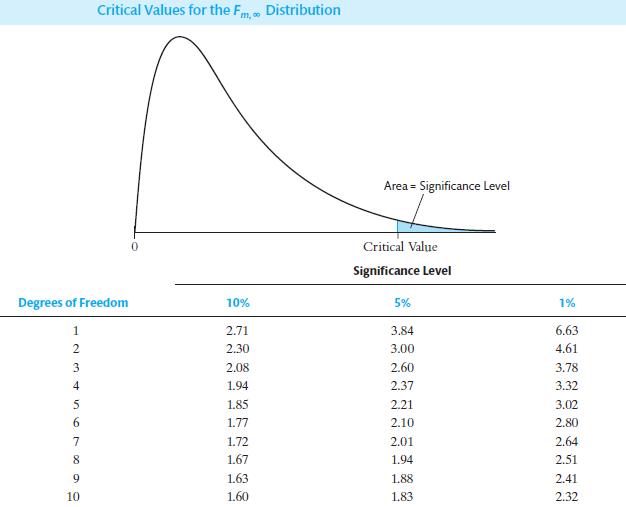
\includegraphics[scale = 0.8]{diplomka obrazky/14.png} 
    \caption{Kritické hodnoty F-rozdelenia pri $df = m$ a $df = \infty$} 
    \source{Zdroj: Source of the image.} 
\end{figure} 

\subsection{F-štatistika s viac ako dvoma reštrikciami}

Uvažujme spojenú hypotézu, ktorá je lineárna v koeficientoch a má $q$ obmedzení, kde $q \leq k + 1$. Každé z týchto $q$ obmedzení môže zahŕňať jeden, alebo viacero regresných koeficientov. Túto spojenú nulovú hypotézu môžeme zapísať v maticovom zápise ako:
\begin{equation}
    R\beta = r,
\end{equation}
kde $R$ je $q \times (k + 1)$ nenáhodná matica s plnou hodnosťou, a $r$ je nenáhodný vektor $q \times 1$. $q$ je počet riadkov v $R$, čo taktiež predstavuje počet obmedzení uvalených pod nulovou hypotézou. 

Vzorec pre F-štatistiku s úpravou pre heteroskedasticitu\footnote{Robustná F-štatistika.} pre testovanie $q$ reštrikcií nulovej hypotézy, ktorý môžeme použiť pre otestovanie nulovej hypotézy v rovnici 11.2 je:
\begin{equation}
    F = (R\hat{\beta}-r)'[R\hat{\sum}_{\hat{\beta}}R']^{-1}(R\hat{\beta}-r)/q,
\end{equation}
kde pri dodržaní prvých štyroch podmienok najmenších štvorcoch platí, že pod nulovou hypotézou:
\begin{equation}
    F \xrightarrow[\text{}]{\text{\; d \; }} F_{q, \infty}.
\end{equation}
Pod nulovou hypotézou má F-štatistika výberové rozdelenie, ktoré je vo veľkých vzorkách určené $F_{q, \infty}$ rozdelením. Teda kritické hodnoty pre F-štatistiku môžeme získať z tabuliek $F_{q, \infty}$ rozdelenia, kde nájdeme požadovanú hodnotu pre $q$ obmedzení a požadovanú hladinu významnosti.
Vzorec pre F-štatistiku s úpravou pre heteroskedasticitu je implementovaný v štatistických softvéroch a nebudeme naň v tejto práci ďalej upriamovať pozornosť. 

\subsection{Celková F-štatistika regresie}

Celková F-štatistika regresie testuje spojenú hypotézu, že všetky koeficienty sklonu sú 0. Nulovú a alternatívnu hypotézu zapíšeme ako:
\begin{equation}
\begin{split}
    H_{0}: & \ \beta_{1} = 0, \beta_{2} = 0, ..., \beta_{k} = 0 \ vs. \\
    H_{1}: & \ \beta_{j} \neq 0, pre \ aspoň \ jedno \ j,\ j=1, ..., k.
\end{split}
\end{equation}
Nulová hypotéza tvrdí, že žiaden z regresorov nevysvetľuje akúkoľvek zmenu v $Y_i$, aj keď priesečník (pod nulovou hypotézou predstavuje priemer $Y_i$) môže byť nenulový. Pri veľkých vzorkách má celková F-štatistika regresie rozdelenie $F_{k,\infty}$, ak je nulová hypotéza pravdivá.

\subsection{F-štatistika s jedným obmedzením}

Keď $q = 1$, F-štatistika testuje iba jedno obmedzenie. Spojená nulová hypotéza sa premení na nulovú hypotézu jedného koeficienta regresie, a F-štatistika bude t-štatistika umocnená na druhú mocninu.  

\subsection{F-štatistika a homoskedasticita}

Ak sú zvyšky regresie homoskedastické, F-štatistiku je možné zapísať v zmysle toho, ako sedia dáta regresii, a to buď poklesom súčtu štvorcov zvyškov, alebo nárastu koeficientu determinácie $R^2$. Výsledná F-štatistika sa uvádza ako F-štatistika pre homoskedasticitu, pretože platí, len ak sú zvyšky regresie homoskedastické. V porovnaní s robustnou F-štatistikou, ktorá platí pri heteroskedastických aj homoskedastických zvyškoch regresie. Aj napriek tomuto obmedzeniu si vzorec pre túto štatistiku predstavíme, kvôli lepšiemu pochopeniu toho, ako F-štatistika vlastne funguje. 

F-štatistiku pre homoskedasticitu vyrátame za použitia jednoduchého vzorca založeného na súčte štvorcov zvyškov z dvoch regresii. Prvá regresia sa nazýva obmedzenou regresiou, v ktorej je nulová hypotéza vynútene pravdivá. Ak je nulová hypotéza typovo ako v rovnici 10.2, teda všetky hodnoty hypotézy sú rovné 0, obmedzená regresia je regresiou, v ktorej sú všetky testované koeficienty nastavené na 0, tým pádom sú príslušné regresory vylúčené z regresie. Druhá regresia sa nazýva neobmedzenou regresiou, v ktorej je alternatívnej hypotéze umožnené byť pravdivou. Ak je súčet štvorcov zvyškov dostatočne menší v neobmedzenej regresií, než v obmedzenej regresií, potom test zamietne nulovú hypotézu. 
F-štatistika pre homoskedasticitu je daná rovnicou:
\begin{equation}
    F= \frac{(SSR_{obmedzená}-SSR_{neobmedzená} / q}{SSR_{neobmedzená}/ (n-k_{neobmedzená}-1)},
\end{equation}
kde:
\begin{itemize}
    \item $SSR_{obmedzená}$ je súčet štvorcov zvyškov z obmedzenej regresie, \item$SSR_{neobmedzená}$ je súčet štvorcov zvyškov z neobmedzenej regresie, 
    \item q je počet obmedzení pod nulovou hypotézou,
    \item $k_{neobmedzená}$ je počet regresorov v neobmedzenom modeli.
\end{itemize}
Ekvivalentom k tejto rovnici je vzorec založený na koeficiente determinácie $R^2$ týchto dvoch regresií:
\begin{equation}
    F= \frac{(R^2_{neobmedzená}-R^2_{obmedzená} / q}{(1 - R^2_{neobmedzená})/ (n-k_{neobmedzená}-1)}.
\end{equation}
Ak sú zvyšky homoskedastické, potom rozdiel medzi F-štatistikou pre homoskedasticitu, vyrátanú poslednými dvoma uvedenými vzorcami, a robustnou F-štatistikou mizne, ako veľkosť vzorky $n$ narastá. Takže, ak sú zvyšky homoskedastické, výberové rozdelenie F-štatistiky pre homoskedasticitu v súlade s nulovou hypotézou, je vo veľkých vzorkách $F_{q,\infty}$. 
\begin{figure}[!ht] 
    \centering 
    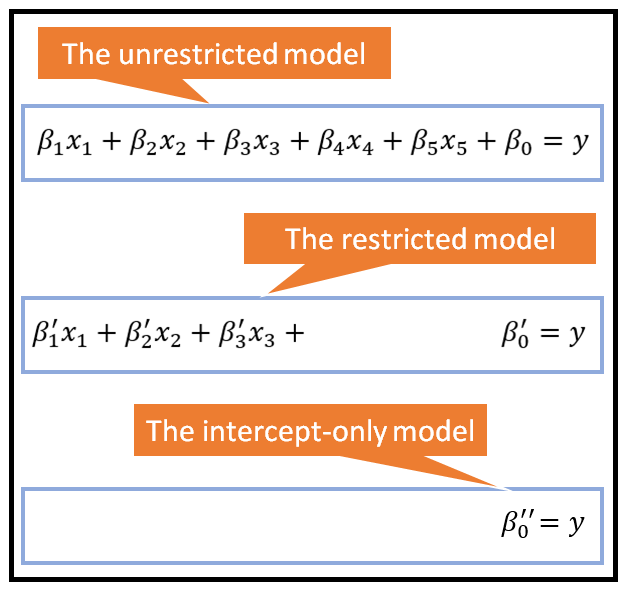
\includegraphics[scale = 0.5]{diplomka obrazky/15.png} 
    \caption{Neobmedzený, obmedzený a iba-priesečník model.} 
    \source{Zdroj: Source of the image.} 
\end{figure} 

\newpage
\section{Špecifikácia modelu viacnásobnej regresie}

Pri odhadovaní kauzálneho efektu potrebujeme určiť, ktoré premenné bude vhodné zahrnúť do modelu. To predstavuje problém výberu špecifikácie regresie. Dôležité je sa taktiež spoľahnúť na vlastnú expertízu a podľa toho voliť premenné, aby sme sa dokázali vyhnúť odchýlke opomenutej premennej. Nie je vhodné sa spoliehať čisto na štatistické ukazovatele, ako napríklad determinačný koeficient.
Viacnásobná regresia nám umožňuje kontrolovať okolnosti, ktoré by mohli viesť k odchýlke opomenutej premennej pri odhade efektu, ktorý nás zaujíma.
Ak chceme určite vhodné kontrolné premenné, vo všeobecnosti nám ako odpoveď poslúži podmienka podmienenej nezávislosti priemernej hodnoty. Teda, na odstránenie odchýlky opomenutej premennej, musí súbor kontrolných premenných spĺňať podmienku
\begin{equation}
    E(u_{t}|X_{t},W_{t}) = E(u_{t}|W_{t}),
\end{equation}
kde $X_{t}$ označuje premennú alebo premenné, ktoré nás zaujímajú, a $W_{t}$ označuje jednu alebo viacero kontrolných premenných.
Tento vzorec znamená, že ak kontrolujeme pre $W$, $X$ nie je závislé od zvyškov regresie, teda je nezávislé od zvyškov. Inak, podmienené očakávanie zvyškov regresie nezávisí na $X$, ak kontrolujeme pre $W$. Podmienený $W$, $X$ je akoby náhodne určené, takže $X$ sa stane nekorelovaným s $u$, avšak $W$ s $u$ korelované byť môže. Keďže v ekonometrii pracujeme s premennými, pri ktorých si nie sme istí, či sú náhodne rozdelené, a nezávislé od náhodnej zložky, používame kontrolné premenné. Ak tento vzťah nebude dodržaný, naďalej sa budú vyskytovať determinanty $Y$, ktoré nie sú zahrnuté v modeli, a sú korelované s $X$ aj napriek tomu, že držíme $W$ konštantné. Výsledkom čoho je odchýlka vynechanej premennej. Za dodržania podmienenej nezávislosti priemeru, nám $OLS$ môže poskytnúť konzistentného odhadcu bez odchýlky pre $X$, avšak nie pre koeficient $W$. 

Zvyčajne sa postupuje v dvoch krokoch. Prvým je základný súbor regresorov, ktorý sme určili na základe znalostí tematiky, ekonomickej teórie a vedomostiach o spôsobe zberu dát. Regresia, ktorá používa tento základný súbor regresorov sa zvykne označovať ako základná špecifikácia. Táto základná špecifikácia by mala obsahovať premenné, ktoré nás zaujímajú a zároveň kontrolné premenné, ktoré sme určili na základe skúseností a ekonomickej teórie. Znalosti a teória však málokedy stačia na úplné zostavenie modelu, keďže k premenným, ktoré by sme ideálne chceli v modeli, nedokážeme zohnať dostatok dát. Tým pádom je ďalším krokom vytvorenie zoznamu kandidátov pre alternatívnu špecifikáciu, alternatívny súbor regresorov. Ak sú odhady koeficientov, premennej záujmu, numericky podobné naprieč alternatívnou špecifikáciou, znamená to, že odhady zo základnej špecifikácie sú spoľahlivé. Naopak, ak sa hodnoty koeficientov výrazne zmenia naprieč alternatívnou špecifikáciou, často to znamená, že základná špecifikácia mala odchýlku vynechanej premennej, čo môže znamenať, že rovnakým problémom bude trpieť aj alternatívna špecifikácia. 

\subsection{Chybná funkčná forma regresie}

Ďalším problémom je výber funkčnej formy regresie. Ak bude model lineárny, avšak vzťah premenných bude nelineárny, nastane skreslenie výsledných koeficientov regresie, čiže regresia nebude vhodne opisovať vzťah medzi premennými. Predísť chybnej špecifikácií funkčnej formy regresie je možné jednoduchým premietnutím dát na graf, a pomocou pozorovania určiť najvhodnejšiu funkčnú formu regresie. Toto chybné určenie funkčnej formy regresie je druh odchýlky vynechanej premennej, kde opomenutá premenná predstavuje chýbajúci nelineárny aspekt regresnej funkcie. 

\section{Záver}

\section{Praktická časť}

% Options for packages loaded elsewhere
\PassOptionsToPackage{unicode}{hyperref}
\PassOptionsToPackage{hyphens}{url}
%
\documentclass[]{article}
\usepackage{lmodern}
\usepackage{subfiles}
\usepackage{amssymb,amsmath}
\usepackage{ifxetex,ifluatex}
\ifnum 0\ifxetex 1\fi\ifluatex 1\fi=0 % if pdftex
  \usepackage[T1]{fontenc}
  \usepackage[utf8]{inputenc}
  \usepackage{textcomp} % provide euro and other symbols
\else % if luatex or xetex
  \usepackage{unicode-math}
  \defaultfontfeatures{Scale=MatchLowercase}
  \defaultfontfeatures[\rmfamily]{Ligatures=TeX,Scale=1}
\fi
% Use upquote if available, for straight quotes in verbatim environments
\IfFileExists{upquote.sty}{\usepackage{upquote}}{}
\IfFileExists{microtype.sty}{% use microtype if available
  \usepackage[]{microtype}
  \UseMicrotypeSet[protrusion]{basicmath} % disable protrusion for tt fonts
}{}
\makeatletter
\@ifundefined{KOMAClassName}{% if non-KOMA class
  \IfFileExists{parskip.sty}{%
    \usepackage{parskip}
  }{% else
    \setlength{\parindent}{0pt}
    \setlength{\parskip}{6pt plus 2pt minus 1pt}}
}{% if KOMA class
  \KOMAoptions{parskip=half}}
\makeatother
\usepackage{xcolor}
\IfFileExists{xurl.sty}{\usepackage{xurl}}{} % add URL line breaks if available
\IfFileExists{bookmark.sty}{\usepackage{bookmark}}{\usepackage{hyperref}}
\hypersetup{
  pdftitle={Praktická časť diplomovej práce},
  hidelinks,
  pdfcreator={LaTeX via pandoc}}
\urlstyle{same} % disable monospaced font for URLs
\usepackage[margin=1in]{geometry}
\usepackage{color}
\usepackage{fancyvrb}
\newcommand{\VerbBar}{|}
\newcommand{\VERB}{\Verb[commandchars=\\\{\}]}
\DefineVerbatimEnvironment{Highlighting}{Verbatim}{commandchars=\\\{\}}
% Add ',fontsize=\small' for more characters per line
\usepackage{framed}
\definecolor{shadecolor}{RGB}{248,248,248}
\newenvironment{Shaded}{\begin{snugshade}}{\end{snugshade}}
\newcommand{\AlertTok}[1]{\textcolor[rgb]{0.94,0.16,0.16}{#1}}
\newcommand{\AnnotationTok}[1]{\textcolor[rgb]{0.56,0.35,0.01}{\textbf{\textit{#1}}}}
\newcommand{\AttributeTok}[1]{\textcolor[rgb]{0.77,0.63,0.00}{#1}}
\newcommand{\BaseNTok}[1]{\textcolor[rgb]{0.00,0.00,0.81}{#1}}
\newcommand{\BuiltInTok}[1]{#1}
\newcommand{\CharTok}[1]{\textcolor[rgb]{0.31,0.60,0.02}{#1}}
\newcommand{\CommentTok}[1]{\textcolor[rgb]{0.56,0.35,0.01}{\textit{#1}}}
\newcommand{\CommentVarTok}[1]{\textcolor[rgb]{0.56,0.35,0.01}{\textbf{\textit{#1}}}}
\newcommand{\ConstantTok}[1]{\textcolor[rgb]{0.00,0.00,0.00}{#1}}
\newcommand{\ControlFlowTok}[1]{\textcolor[rgb]{0.13,0.29,0.53}{\textbf{#1}}}
\newcommand{\DataTypeTok}[1]{\textcolor[rgb]{0.13,0.29,0.53}{#1}}
\newcommand{\DecValTok}[1]{\textcolor[rgb]{0.00,0.00,0.81}{#1}}
\newcommand{\DocumentationTok}[1]{\textcolor[rgb]{0.56,0.35,0.01}{\textbf{\textit{#1}}}}
\newcommand{\ErrorTok}[1]{\textcolor[rgb]{0.64,0.00,0.00}{\textbf{#1}}}
\newcommand{\ExtensionTok}[1]{#1}
\newcommand{\FloatTok}[1]{\textcolor[rgb]{0.00,0.00,0.81}{#1}}
\newcommand{\FunctionTok}[1]{\textcolor[rgb]{0.00,0.00,0.00}{#1}}
\newcommand{\ImportTok}[1]{#1}
\newcommand{\InformationTok}[1]{\textcolor[rgb]{0.56,0.35,0.01}{\textbf{\textit{#1}}}}
\newcommand{\KeywordTok}[1]{\textcolor[rgb]{0.13,0.29,0.53}{\textbf{#1}}}
\newcommand{\NormalTok}[1]{#1}
\newcommand{\OperatorTok}[1]{\textcolor[rgb]{0.81,0.36,0.00}{\textbf{#1}}}
\newcommand{\OtherTok}[1]{\textcolor[rgb]{0.56,0.35,0.01}{#1}}
\newcommand{\PreprocessorTok}[1]{\textcolor[rgb]{0.56,0.35,0.01}{\textit{#1}}}
\newcommand{\RegionMarkerTok}[1]{#1}
\newcommand{\SpecialCharTok}[1]{\textcolor[rgb]{0.00,0.00,0.00}{#1}}
\newcommand{\SpecialStringTok}[1]{\textcolor[rgb]{0.31,0.60,0.02}{#1}}
\newcommand{\StringTok}[1]{\textcolor[rgb]{0.31,0.60,0.02}{#1}}
\newcommand{\VariableTok}[1]{\textcolor[rgb]{0.00,0.00,0.00}{#1}}
\newcommand{\VerbatimStringTok}[1]{\textcolor[rgb]{0.31,0.60,0.02}{#1}}
\newcommand{\WarningTok}[1]{\textcolor[rgb]{0.56,0.35,0.01}{\textbf{\textit{#1}}}}
\usepackage{longtable,booktabs}
% Correct order of tables after \paragraph or \subparagraph
\usepackage{etoolbox}
\makeatletter
\patchcmd\longtable{\par}{\if@noskipsec\mbox{}\fi\par}{}{}
\makeatother
% Allow footnotes in longtable head/foot
\IfFileExists{footnotehyper.sty}{\usepackage{footnotehyper}}{\usepackage{footnote}}
\makesavenoteenv{longtable}
\usepackage{graphicx,grffile}
\makeatletter
\def\maxwidth{\ifdim\Gin@nat@width>\linewidth\linewidth\else\Gin@nat@width\fi}
\def\maxheight{\ifdim\Gin@nat@height>\textheight\textheight\else\Gin@nat@height\fi}
\makeatother
% Scale images if necessary, so that they will not overflow the page
% margins by default, and it is still possible to overwrite the defaults
% using explicit options in \includegraphics[width, height, ...]{}
\setkeys{Gin}{width=\maxwidth,height=\maxheight,keepaspectratio}
% Set default figure placement to htbp
\makeatletter
\def\fps@figure{htbp}
\makeatother
\setlength{\emergencystretch}{3em} % prevent overfull lines
\providecommand{\tightlist}{%
  \setlength{\itemsep}{0pt}\setlength{\parskip}{0pt}}
\setcounter{secnumdepth}{5}

\title{Praktická časť diplomovej práce}
\author{}
\date{\vspace{-2.5em}}

\begin{document}

\maketitle

\hypertarget{sprievodca-ekfmetriou}{%
\section{Sprievodca ekfmetriou}\label{sprievodca-ekfmetriou}}

Sprievodca ekonometriou má za úlohu priblížiť Vám ekonometriu, a pomôcť
Vám jej porozumieť. Sprievodcu píšem ako študent, ktorý sa ekonometriu
začal učiť sám, a sám si prešiel zdĺhavým procesom bádania a
usmerňovania. Sprievodca je zostrojený ako-tak súbežne s osnovou a
zadaniami, ktoré obdržíte na hodine. Nebudeme sa konkrétne držať
vypracovania zadaní, ale skôr princípmi, z ktorých zadania ťažia. Mnoho
študentov tento predmet nezaujíma, a zadania vypracujú okopírovaním
postupov starších spolužiakov, nuž, pochopiť ekonometriu a jej postupy
nie je vôbec jednoduché, a dokážem pochopiť, keď si študenti hľadajú
skratky. Na druhú stranu, ekonometria predstavuje skvelú vstupnú bránu
do sveta analytiky. Človek je zavalený Machine Learningom, Data Sciencom
a AI-čkom, nuž až po sfúknutí pozlátka zistí, že je to zmes matematiky,
štatistiky a počítačovej vedy. Ekonometria je teda skvelou výhovorkou,
ako oprášiť matematiku, doučiť sa štatistiku, a naučiť sa troška
programovania. R-ko sa môže zdať ako jazyk, ktorý žije v tieni Pythonu,
avšak, akoby nejedna Dominika vedela dosvedčiť, netreba sa nechať
voviesť do omylu. R-ko je najvhodnejší programovací jazyk pre
štatistikov, Google ho zahrnul do najnovších kurzov Google Analytics.
Mojou úlohou je pomôcť Vám prekonať problém, ktorý som na začiatku
svojej cesty ekonometriou vôbec nepovažoval za problém, a to množstvo
materiálov, ktoré zavalí študenta. Pomôžem Vám postupne zložiť skladačku
konceptov a teórií, na ktorých ekonometria stojí. Náročnosť
prezentovania konceptov bude prispôsobená, nehnevajte sa, keď neskôr
objavíte niečo, čo som spomenúť mohol, ale nespomenul. Nemá zmysel
vysvetľovať odvodzovanie každého estimátora. Cieľom je poskytnúť
všeobecný náhľad ekonometrie, a pomôcť Vám pochopiť, a príjemnejšie
zvládnuť predmet Ekonometria.

~

\textbf{Čo nás čaká:}

\begin{enumerate}
\def\labelenumi{\arabic{enumi}.}
\tightlist
\item
  Základy programovania v R
\item
  Ekonometrické techniky
\item
  Intuitívny prehľad štatistických konceptov
\end{enumerate}

\newpage

\hypertarget{zuxe1klady-programovania-v-r}{%
\section{Základy programovania v R}\label{zuxe1klady-programovania-v-r}}

\begin{quote}
Sprievodca je interaktívny, teda začneme stiahnutím a inštaláciou
\href{https://cran.r-project.org/mirrors.html}{R} a
\href{https://cran.r-project.org/mirrors.html}{RStudia}. R má samo o
sebe programovacie prostredie, avšak dnešným štandardom je používanie
intregrovaného vývojového prostredia (IDE) v podobe RStudia.
\end{quote}

\hypertarget{aritmetickuxe9-operuxe1tory}{%
\subsection{Aritmetické operátory}\label{aritmetickuxe9-operuxe1tory}}

\emph{Poďme teda rovno na vec. Začneme základnými funkciami.} R môžeme
používať ako kalkulačku, teda za pomoci klasických aritmetických
operátorov môžeme sčítať, odčítať, násobiť, deliť či umocňovať:

\begin{Shaded}
\begin{Highlighting}[]
\DecValTok{5} \OperatorTok{+}\StringTok{ }\DecValTok{5}
\end{Highlighting}
\end{Shaded}

\begin{verbatim}
## [1] 10
\end{verbatim}

\begin{Shaded}
\begin{Highlighting}[]
\DecValTok{5} \OperatorTok{-}\StringTok{ }\DecValTok{5}
\end{Highlighting}
\end{Shaded}

\begin{verbatim}
## [1] 0
\end{verbatim}

\begin{Shaded}
\begin{Highlighting}[]
\DecValTok{5} \OperatorTok{*}\StringTok{ }\DecValTok{5}
\end{Highlighting}
\end{Shaded}

\begin{verbatim}
## [1] 25
\end{verbatim}

\begin{Shaded}
\begin{Highlighting}[]
\DecValTok{5} \OperatorTok{/}\StringTok{ }\DecValTok{5}
\end{Highlighting}
\end{Shaded}

\begin{verbatim}
## [1] 1
\end{verbatim}

\begin{Shaded}
\begin{Highlighting}[]
\DecValTok{5}\OperatorTok{^}\DecValTok{2}
\end{Highlighting}
\end{Shaded}

\begin{verbatim}
## [1] 25
\end{verbatim}

R-ko dokáže používať aj ďalšie aritmetické operátory:

\begin{Shaded}
\begin{Highlighting}[]
\CommentTok{# zobrazí zvyšok z delenia}

\DecValTok{5} \OperatorTok\StringTok{ }\DecValTok{2}
\end{Highlighting}
\end{Shaded}

\begin{verbatim}
## [1] 1
\end{verbatim}

My sa budeme zapodievať len tým, s čím sa na cvičeniach stretneme. Našou
úlohou nie je naučiť sa dokonalo ovládať R, ale naučiť sa používať ho v
dostatočnej miere, aby sme s ním zvládli to, čo budeme v najbližšej dobe
potrebovať.

\newpage

\hypertarget{baluxedky}{%
\subsection{Balíky}\label{baluxedky}}

Okrem základných operátorov budeme využívať aj funkcie:

\begin{Shaded}
\begin{Highlighting}[]
\KeywordTok{mean}\NormalTok{(}\DecValTok{2}\NormalTok{, }\DecValTok{4}\NormalTok{, }\DecValTok{6}\NormalTok{)}
\end{Highlighting}
\end{Shaded}

\begin{verbatim}
## [1] 2
\end{verbatim}

\begin{Shaded}
\begin{Highlighting}[]
\KeywordTok{abs}\NormalTok{(}\OperatorTok{-}\DecValTok{5}\NormalTok{)}
\end{Highlighting}
\end{Shaded}

\begin{verbatim}
## [1] 5
\end{verbatim}

\begin{Shaded}
\begin{Highlighting}[]
\KeywordTok{sqrt}\NormalTok{(}\DecValTok{8}\NormalTok{)}
\end{Highlighting}
\end{Shaded}

\begin{verbatim}
## [1] 2.828427
\end{verbatim}

Tieto funkcie sa nachádzajú v balíkoch, ktoré si môžeme predstaviť ako
také Addony. R figuruje balíkmi, ktoré sú predinštalované, a zahŕňajú
najpoužívanejšie a najzákladnejšie funkcie. Vyššie použíté funkcie sa
nachádzajú v balíku base. To, v akom balíku sa funkcia nachádza zistíte
po napísaní funkcie

~

\begin{center}


\includegraphics{diplomka obrazky/1.png}

\end{center}

~

to však len zapredpokladu, že už máte balík nainštalovaný. Ak narazíte
na názov funkcie, ktorú chcete použiť, avšak nemáte nainštalovaný balík
a chcete zistiť jeho názov, buď si funkciu zadajte do Google, alebo
napíšte do konzoly:

\begin{Shaded}
\begin{Highlighting}[]
\CommentTok{# ??meno funkcie}

\NormalTok{??mean}
\end{Highlighting}
\end{Shaded}

My budeme často využívať predinštalované balíky \textbf{base} a
\textbf{stats}, avšak za pochodu si budeme inštalovať aj ďalšie balíky,
s ktorými sa na cvičeniach stretnete. Nový balík je potrebné prv
nainštalovať a potom ho načítať do prostredia.

\begin{Shaded}
\begin{Highlighting}[]
\CommentTok{# stiahneme a našintalujeme pomocou R konzoly a funkcie install.packages()}
\CommentTok{# ! názov balíka je citlivý na veľkosť písma}
\CommentTok{# ! názov musí byť v úvodzovkách}

\KeywordTok{install.packages}\NormalTok{(}\StringTok{"fBasics"}\NormalTok{)}

\CommentTok{# po nainštalovaní máme balík stiahnutý v našom PC, a tento príkaz už viac nepoužívame}
\CommentTok{# ak však chceme funkcie z balíka použiť, musíme po zapnutí R-ka balík načítať príkazom}

\KeywordTok{library}\NormalTok{(fBasics)}

\CommentTok{# ! tu už úvodzovky nie sú potrebné}
\end{Highlighting}
\end{Shaded}

\begin{quote}
\emph{Pri inštalovaní názov balíka zabalíme do úvodzoviek. Pri jeho
načítaní pomocou library() už úvodzovky nepíšeme. Na pohovor si vezmeme
oblek (úvodzovky), ale po prijatí už chodíme do práce bez obleku.}
\end{quote}

\hypertarget{objekty}{%
\subsection{Objekty}\label{objekty}}

Často chceme vyrátané výsledky znova použiť, a preto by bolo vhodné si
ich niekde uložiť. Na ukladanie a uskladnenie výsledkov slúžia objekty.
Každý objekt má meno a obsah. Meno si môžeme zadať akékoľvek, musí však:

\begin{itemize}
\tightlist
\item
  začínať malým alebo veľkým písmenom a nie číslom
\item
  obsahovať iba čísla, písmená alebo niektoré špeciálne znaky ako
  \("."\) či "\_".
\end{itemize}

\begin{quote}
\emph{Nezabúdajme, že R je case sensitive (rozlišuje veľké a malé
písmená).}
\end{quote}

Povedzme že chceme vytvoriť objekt \textbf{a} a priradiť mu hodnotu
\(2 + 2\). Na priradenie obsahu je možné použiť \("="\), avšak
štandardom je používanie \("<-"\).

\begin{quote}
\emph{Znak \textless- nie je nutné písať dvoma znakmi, používa sa na to
skratka \textbf{``ľavý Alt'' a ``-''}. Na SK klávesnici nájdeme znak
naľavo od pravého Shiftu, na EN klávesnici zvyčajne naľavo od Backspacu.
Osobne programujem s EN klávesnicou, nech som použíteľný v akomkoľvek
štáte bez potreby inštalovať SK klávesnicu.}
\end{quote}

\begin{Shaded}
\begin{Highlighting}[]
\CommentTok{# Priradíme teda objektu "a" výsledok "2 + 2".}

\NormalTok{a <-}\StringTok{ }\DecValTok{2} \OperatorTok{+}\StringTok{ }\DecValTok{2}

\CommentTok{# Po napísaní názvu objektu do konzoly nám konzola ukáže už len výsledok.}

\NormalTok{a}
\end{Highlighting}
\end{Shaded}

\begin{verbatim}
## [1] 4
\end{verbatim}

\begin{Shaded}
\begin{Highlighting}[]
\CommentTok{# Nové priradenie hodnoty starému objektu prepíše starú hodnotu.}

\NormalTok{a <-}\StringTok{ }\DecValTok{5} \OperatorTok{+}\StringTok{ }\DecValTok{5}

\NormalTok{a}
\end{Highlighting}
\end{Shaded}

\begin{verbatim}
## [1] 10
\end{verbatim}

S daným objektom môžeme pracovať, akoby to bola číselná hodnota.

\begin{Shaded}
\begin{Highlighting}[]
\NormalTok{a}\OperatorTok{^}\DecValTok{2}
\end{Highlighting}
\end{Shaded}

\begin{verbatim}
## [1] 100
\end{verbatim}

\newpage

\hypertarget{vektory}{%
\subsection{Vektory}\label{vektory}}

Pre priradenie viacerých hodnôt vytvoríme vektor. Vektor vytvoríme
pomocou funkcie c() ako combine.

\begin{Shaded}
\begin{Highlighting}[]
\CommentTok{# Objektu "a" priradíme súbor číselných hodnôt a vytvoríme z neho vektor.}

\NormalTok{a <-}\StringTok{ }\KeywordTok{c}\NormalTok{(}\DecValTok{5}\NormalTok{, }\DecValTok{1}\NormalTok{, }\DecValTok{4}\NormalTok{, }\DecValTok{2}\NormalTok{, }\DecValTok{3}\NormalTok{)}

\NormalTok{a}
\end{Highlighting}
\end{Shaded}

\begin{verbatim}
## [1] 5 1 4 2 3
\end{verbatim}

S vektormi dokážeme rôzne pracovať. Sčítavať, násobiť, aplikovať na ne
funkcie, všetko, čo nás napadne. Ups, čo nám napadne!

\begin{Shaded}
\begin{Highlighting}[]
\NormalTok{b <-}\StringTok{ }\KeywordTok{c}\NormalTok{(}\DecValTok{5}\NormalTok{, }\DecValTok{9}\NormalTok{, }\DecValTok{6}\NormalTok{, }\DecValTok{8}\NormalTok{, }\DecValTok{7}\NormalTok{)}
\NormalTok{a }\OperatorTok{+}\StringTok{ }\NormalTok{b}
\end{Highlighting}
\end{Shaded}

\begin{verbatim}
## [1] 10 10 10 10 10
\end{verbatim}

\begin{Shaded}
\begin{Highlighting}[]
\KeywordTok{min}\NormalTok{(a)}
\end{Highlighting}
\end{Shaded}

\begin{verbatim}
## [1] 1
\end{verbatim}

\begin{Shaded}
\begin{Highlighting}[]
\KeywordTok{sort}\NormalTok{(a)}
\end{Highlighting}
\end{Shaded}

\begin{verbatim}
## [1] 1 2 3 4 5
\end{verbatim}

\begin{Shaded}
\begin{Highlighting}[]
\KeywordTok{sum}\NormalTok{(a)}
\end{Highlighting}
\end{Shaded}

\begin{verbatim}
## [1] 15
\end{verbatim}

Je vhodné poznať pár špeciálnych funkcií na tvorbu vektorov. A to:

\begin{Shaded}
\begin{Highlighting}[]
\CommentTok{# sample(), seq() a rep()}
\end{Highlighting}
\end{Shaded}

Často si totižto potrebujete vytvoriť vektor hodnôt podľa vlastnej
potreby. Hm, to som veľmi nič nové nepovedal. Ale\ldots{} Čo vlastne
tieto funkcie robia? A ako to zistíme? Ak pracujete s úplne novou
funkciou, a máte už nainštalovaný balík, a taktiež ste ho už načítali do
knižnice cez \(library()\), je vhodné použiť \(?názovfunkcie\) alebo
\(help(názovfunkcie)\). Poskytne Vám to stručný popis, čo funkcia robí,
všetky jej argumeny a aj pár príkladov. Ak už ste však s funkciou
pracovali, ale nepamätáte si argumenty, rozpíšte funkciu, kliknite sa do
zátvoriek funkcie \(mean(tu.sa.kliknete)\), a stlačíte \(TAB\). Vyhodí
Vám to argumenty funkcie. Skúsime si to na funkcii \(sample()\).

~

\hypertarget{sample}{%
\subsubsection{sample()}\label{sample}}

\begin{center}

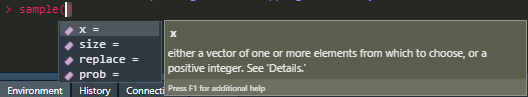
\includegraphics[width=0.85\textwidth,height=\textheight]{diplomka obrazky/2.png}

\end{center}

~

Pri jednej z vecí, ktorú Vám chcem ukázať, budeme potrebovať vektor
výšky ľudí. Tak si ho teda vytvorme už teraz. Ešte predtým môžeme skúsiť
napísať do konzoly \(?sample\), čím zistíme, že funkcia \(sample()\) nám
náhodne vyberie hodnoty zo zadaného vektora.

~

\begin{center}

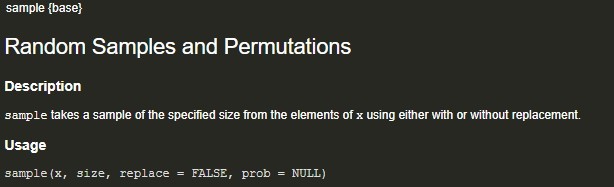
\includegraphics[width=0.8\textwidth,height=\textheight]{diplomka obrazky/3.png}

\end{center}

~

\begin{Shaded}
\begin{Highlighting}[]
\CommentTok{# Ako prvé potrebujeme zadať "x", teda vektor hodnôt, z ktorých chceme vyberať.}
\CommentTok{# Pre nás to budú hodnoty medzi 160 až 190, ktoré navolíme ako 160:190.}

\CommentTok{# 160:190 jednoducho vypíše hodnoty zaradom od 160 do 190. A sample() z nich náhodne vyberie}
\CommentTok{# nami určený počet hodnôt.}


\CommentTok{# "size" je počet hodnôt, aký ma funkcia vybrať.}

\CommentTok{# "replace", či môže vybrať jednu hodnotu viackrát, alebo ju má vylúčiť.}

\CommentTok{# "prob" použijeme, ak chceme priradiť istým hodnotám inú váhu.}

\NormalTok{vyska <-}\StringTok{ }\KeywordTok{sample}\NormalTok{(}\DataTypeTok{x =} \DecValTok{160}\OperatorTok{:}\DecValTok{190}\NormalTok{, }\DataTypeTok{size =} \DecValTok{10}\NormalTok{, }\DataTypeTok{replace =} \OtherTok{TRUE}\NormalTok{)}

\KeywordTok{print}\NormalTok{(vyska)}
\end{Highlighting}
\end{Shaded}

\begin{verbatim}
##  [1] 174 184 161 166 164 174 172 188 170 173
\end{verbatim}

\begin{quote}
\emph{Funkcia by fungovala, aj keby sme to napísali ako}
``sample(160:190, 10, TRUE)''. \emph{Je však vhodné písať aj argumenty.
Hlavne pri funkciách, ktoré nie sú veľmi bežné. Ak po Vás niekto bude
čítať kód, číta sa to lepšie.}
\end{quote}

\newpage

\hypertarget{seq}{%
\subsubsection{seq()}\label{seq}}

Funkcia \(seq()\) vygeneruje sekvenciu čísel. Ako argumenty zadávame buď
\(od\), \(do\) a \(by\). Teda po akých inkrementoch bude daná sekvencia
narastať.

\begin{Shaded}
\begin{Highlighting}[]
\KeywordTok{seq}\NormalTok{(}\DataTypeTok{from =} \DecValTok{2}\NormalTok{, }\DataTypeTok{to =} \DecValTok{12}\NormalTok{, }\DataTypeTok{by =} \FloatTok{0.5}\NormalTok{)}
\end{Highlighting}
\end{Shaded}

\begin{verbatim}
##  [1]  2.0  2.5  3.0  3.5  4.0  4.5  5.0  5.5  6.0  6.5  7.0  7.5  8.0  8.5  9.0
## [16]  9.5 10.0 10.5 11.0 11.5 12.0
\end{verbatim}

~

\begin{quote}
\emph{V Rku používame na oddeľovanie desatiných miest bodku. Čiarkou
oddeľujeme argumenty. Taktiež nezabúdajte používať medzery. Jedná sa o
gramatiku programovania. Predsalen náš vyššie napísaný výraz vyzerá
lepšie ako} seq(from=2,to=12,by=0.5).
\end{quote}

~

\begin{Shaded}
\begin{Highlighting}[]
\CommentTok{# Zadáme "od", "do" a koľko časí má vektor mať.}

\KeywordTok{seq}\NormalTok{(}\DataTypeTok{from =} \DecValTok{4}\NormalTok{, }\DataTypeTok{to =} \DecValTok{10}\NormalTok{, }\DataTypeTok{length =} \DecValTok{4}\NormalTok{) }
\end{Highlighting}
\end{Shaded}

\begin{verbatim}
## [1]  4  6  8 10
\end{verbatim}

\begin{Shaded}
\begin{Highlighting}[]
\KeywordTok{seq}\NormalTok{(}\DataTypeTok{from =} \DecValTok{4}\NormalTok{, }\DataTypeTok{to =} \DecValTok{10}\NormalTok{, }\DataTypeTok{length =} \DecValTok{8}\NormalTok{)}
\end{Highlighting}
\end{Shaded}

\begin{verbatim}
## [1]  4.000000  4.857143  5.714286  6.571429  7.428571  8.285714  9.142857
## [8] 10.000000
\end{verbatim}

\begin{Shaded}
\begin{Highlighting}[]
\CommentTok{# Alternatívou je zadať "od", "po", a rozdeliť to po požadovaných kúskoch}
\CommentTok{# na požadovanú dĺžku.}

\KeywordTok{seq}\NormalTok{(}\DataTypeTok{from =} \DecValTok{4}\NormalTok{, }\DataTypeTok{by =} \FloatTok{0.5}\NormalTok{, }\DataTypeTok{length =} \DecValTok{25}\NormalTok{)}
\end{Highlighting}
\end{Shaded}

\begin{verbatim}
##  [1]  4.0  4.5  5.0  5.5  6.0  6.5  7.0  7.5  8.0  8.5  9.0  9.5 10.0 10.5 11.0
## [16] 11.5 12.0 12.5 13.0 13.5 14.0 14.5 15.0 15.5 16.0
\end{verbatim}

\hypertarget{rep}{%
\subsubsection{rep()}\label{rep}}

Funkcie \(rep()\) jednoducho zopakuje zadané číslo, alebo vektor,
x-krát.

\begin{Shaded}
\begin{Highlighting}[]
\KeywordTok{rep}\NormalTok{(}\DataTypeTok{x =} \DecValTok{1}\NormalTok{, }\DataTypeTok{times =} \DecValTok{10}\NormalTok{)}
\end{Highlighting}
\end{Shaded}

\begin{verbatim}
##  [1] 1 1 1 1 1 1 1 1 1 1
\end{verbatim}

\begin{Shaded}
\begin{Highlighting}[]
\KeywordTok{rep}\NormalTok{(}\DataTypeTok{x =} \KeywordTok{c}\NormalTok{(}\DecValTok{1}\NormalTok{, }\DecValTok{2}\NormalTok{, }\DecValTok{3}\NormalTok{), }\DataTypeTok{times =} \DecValTok{3}\NormalTok{)}
\end{Highlighting}
\end{Shaded}

\begin{verbatim}
## [1] 1 2 3 1 2 3 1 2 3
\end{verbatim}

\hypertarget{indexovanie}{%
\subsection{Indexovanie}\label{indexovanie}}

Indexovanie je v R-ku veľmi užitočný spôsob selektovania dát. Ide
jednoducho o výber súboru dát, zo súboru dát. Indexujeme za použitia
hranatých zátvoriek, ktoré bez medzery nalepíme k objektu, z ktorého
chceme dáta vybrať. Najjednoduchšie sa to vysvetľuje ukážkou. A
nezabúdajte, že R-ko začína od jednotky, nie od nuly. Aj keď nám,
ekonómom neprogramátorom to asi ani nepríde divné.

\begin{Shaded}
\begin{Highlighting}[]
\CommentTok{# Vytvorme si obyčajný číselný vektor.}

\NormalTok{obycajny_vektor <-}\StringTok{ }\KeywordTok{c}\NormalTok{(}\DecValTok{1}\OperatorTok{:}\DecValTok{10}\NormalTok{)}

\NormalTok{obycajny_vektor}
\end{Highlighting}
\end{Shaded}

\begin{verbatim}
##  [1]  1  2  3  4  5  6  7  8  9 10
\end{verbatim}

\begin{Shaded}
\begin{Highlighting}[]
\CommentTok{# Za použitia indexovania môžeme vybrať akúkoľvek hodnotu. Chceme vybrať prvú.}

\NormalTok{obycajny_vektor[}\DecValTok{1}\NormalTok{]}
\end{Highlighting}
\end{Shaded}

\begin{verbatim}
## [1] 1
\end{verbatim}

\begin{Shaded}
\begin{Highlighting}[]
\CommentTok{# Alebo súbor hodnôt. Vyberieme prvú a poslednú hodnotu.}

\NormalTok{obycajny_vektor[}\KeywordTok{c}\NormalTok{(}\DecValTok{1}\NormalTok{, }\DecValTok{10}\NormalTok{)]}
\end{Highlighting}
\end{Shaded}

\begin{verbatim}
## [1]  1 10
\end{verbatim}

Pravdepodobne by väčšina z vás napísala \(obycajny\_vektor[1, 10]\), to
by vám však vyhodilo chybu. Prečo je tomu tak plne pochopíte, keď si
ukážeme matice. Aj keď to nie je nič zložité. Vektor si predstavme ako
šípku, ktorá určuje smer. Je to teda, v našom prípade, reťazec čísel,
jedna dlhá šnúra, ktorá nemá žiadne riadky ani stĺpce. R-ko však to, čo
napíšeme do hranatých zátvoriek vníma ako:

\[[riadok, stĺpec]\]\\
\[[row, column]\]

\begin{quote}
\emph{Zo začiatku sa mi zvyklo pliesť, čo ide prvé. Zapamätal som si to
ako RC autíčko. Také tie malé na ovládanie.}
\end{quote}

Čiže prvý údaj predstavuje riadok, a druhý údaj stĺpec. Ak by sme
napísali \([1, 10]\), R-ko by hľadalo v pŕvom riadku desiatu hodnotu. Do
hranatých zátvoriek píšeme vlastne \textbf{súradnice}. V reťazci hodnôt
máme ale iba reťazec hodnôt. (:D) Preto je potrebné použiť funkciu
\(c()\), aby R-ko vedelo, že má vyberať z reťazca hodnôt. Indexovanie je
veeeľmi užitočné, a dá sa využiť veľmi kreatívne. Nám však stačí vedieť,
čo to plus-mínus robí. Aby ste vedeli, čo sa deje, keď uvidíte hranaté
zátvorky. O indexovaní si ešte povieme pri maticiach.

\begin{Shaded}
\begin{Highlighting}[]
\CommentTok{# Indexovaním môžeme aj odobrať hodnotu. Napr., ak chceme všetky okrem poslednej:}

\NormalTok{obycajny_vektor[}\OperatorTok{-}\DecValTok{10}\NormalTok{]}
\end{Highlighting}
\end{Shaded}

\begin{verbatim}
## [1] 1 2 3 4 5 6 7 8 9
\end{verbatim}

\hypertarget{inuxe9-typy-vektorov}{%
\subsection{Iné typy vektorov}\label{inuxe9-typy-vektorov}}

Vektory nemusia obsahovať len čísla. Môžu obsahovať napríklad aj
\textbf{textové} alebo \textbf{logické} premenné. Existuje ešte aj
štvrtý typ, \textbf{faktorové} vektory, ktorým sa ale nebudeme zaoberať.

\hypertarget{vektor-textovuxfdch-premennuxfdch}{%
\subsubsection{Vektor textových
premenných}\label{vektor-textovuxfdch-premennuxfdch}}

\begin{Shaded}
\begin{Highlighting}[]
\CommentTok{# Pre vytvorenie vektora obsahujúceho textové reťazce, musí byť obsah ohraničený}
\CommentTok{# úvodzovkami "".}

\NormalTok{vector_characters <-}\StringTok{ }\KeywordTok{c}\NormalTok{(}\StringTok{"c"}\NormalTok{, }\StringTok{"musíme"}\NormalTok{, }\StringTok{"používať"}\NormalTok{, }\StringTok{"stále"}\NormalTok{, }\StringTok{"ak"}\NormalTok{, }\StringTok{"chceme"}\NormalTok{,}
                       \StringTok{"viac"}\NormalTok{, }\StringTok{"hodnôt"}\NormalTok{)}

\NormalTok{vector_characters}
\end{Highlighting}
\end{Shaded}

\begin{verbatim}
## [1] "c"        "musíme"   "používat" "stále"    "ak"       "chceme"   "viac"    
## [8] "hodnôt"
\end{verbatim}

Vektor tvorený textovým reťazcom nájde svoje uplatnenie napríklad pri
pomenovaní hodnôt.

\begin{Shaded}
\begin{Highlighting}[]
\NormalTok{nazvy <-}\StringTok{ }\KeywordTok{c}\NormalTok{(}\StringTok{"prvy"}\NormalTok{, }\StringTok{"druhy"}\NormalTok{, }\StringTok{"treti"}\NormalTok{)}
\NormalTok{cisla <-}\StringTok{ }\KeywordTok{c}\NormalTok{(}\DecValTok{1}\NormalTok{, }\DecValTok{2}\NormalTok{, }\DecValTok{3}\NormalTok{)}

\CommentTok{# Použijeme na to funkciu names()}

\KeywordTok{names}\NormalTok{(cisla) <-}\StringTok{ }\NormalTok{nazvy}

\CommentTok{# Ak sa teraz pozrieme na vektor "cisla", uvidíme, že sme číslam priradili názvy.}
\CommentTok{# Na vypísanie výsledku môžeme použíť aj funkciu print().}

\KeywordTok{print}\NormalTok{(cisla)}
\end{Highlighting}
\end{Shaded}

\begin{verbatim}
##  prvy druhy treti 
##     1     2     3
\end{verbatim}

Vektor \textbf{``cisla''} sme vlozili do funkcie \textbf{names()}.
Aplikovali sme funkciu na vektor, ktorému sme chceli priradiť názvy.
\textbf{Priradiť}, teda symbol priradenia \textbf{\textless-}, potom už
len vektor s názvami, ktoré chceme priradiť. Pre lepšiu ilustráciu si to
napíšeme nanovo, bez zadefinovaného vektora ``nazvy''.

\begin{Shaded}
\begin{Highlighting}[]
\KeywordTok{names}\NormalTok{(cisla) <-}\StringTok{ }\KeywordTok{c}\NormalTok{(}\StringTok{"adin"}\NormalTok{, }\StringTok{"dos"}\NormalTok{, }\StringTok{"tres"}\NormalTok{)}

\KeywordTok{print}\NormalTok{(cisla)}
\end{Highlighting}
\end{Shaded}

\begin{verbatim}
## adin  dos tres 
##    1    2    3
\end{verbatim}

\newpage

\hypertarget{vektor-logickuxfdch-premennuxfdch}{%
\subsubsection{Vektor logických
premenných}\label{vektor-logickuxfdch-premennuxfdch}}

\begin{Shaded}
\begin{Highlighting}[]
\CommentTok{# Logické operátory, inak známe ako Booleovské operátory, nám ako výsledok}
\CommentTok{# poskytnú výstup v podobe TRUE alebo FALSE.}
\CommentTok{# ! Pre overenie rovnosti použijeme "==".}

\NormalTok{vektor <-}\StringTok{  }\DecValTok{5}

\NormalTok{vektor }\OperatorTok{==}\StringTok{ }\DecValTok{5}
\end{Highlighting}
\end{Shaded}

\begin{verbatim}
## [1] TRUE
\end{verbatim}

\begin{Shaded}
\begin{Highlighting}[]
\NormalTok{vektor }\OperatorTok{==}\StringTok{ }\DecValTok{6}
\end{Highlighting}
\end{Shaded}

\begin{verbatim}
## [1] FALSE
\end{verbatim}

~

\begin{longtable}[]{@{}ll@{}}
\toprule
Logický operátor & Popis\tabularnewline
\midrule
\endhead
\textless{} & menšie než\tabularnewline
\textless= & menšie alebo rovné\tabularnewline
\textgreater{} & väčšie než\tabularnewline
\textgreater= & väčšie alebo rovné\tabularnewline
== & rovná sa\tabularnewline
!= & nerovná sa\tabularnewline
!x & nie je x\tabularnewline
x & y\tabularnewline
x \& y & x a y\tabularnewline
isTRUE(x) & test či je x pravdivé\tabularnewline
\bottomrule
\end{longtable}

~

Logické operátory sa zídu pri indexovaní, alebo pri zisťovaní počtu
vyhovujúcich hodnôt.

\begin{Shaded}
\begin{Highlighting}[]
\CommentTok{# Vektor výšky ľudí, ktorý sme si skôr vytvorili.}

\NormalTok{vyska <-}\StringTok{ }\KeywordTok{sample}\NormalTok{(}\DataTypeTok{x =} \DecValTok{160}\OperatorTok{:}\DecValTok{190}\NormalTok{, }\DataTypeTok{size =} \DecValTok{10}\NormalTok{, }\DataTypeTok{replace =} \OtherTok{TRUE}\NormalTok{)}

\CommentTok{# Použitie logického operátora na zistenie, kto má viac ako 170cm. }

\NormalTok{viac_ako_}\DecValTok{170}\NormalTok{ <-}\StringTok{ }\NormalTok{vyska }\OperatorTok{>}\StringTok{ }\DecValTok{170}

\CommentTok{# Výsledky však nebudú číselnými hodnotami, ale hodnotami booleovského typu.}

\KeywordTok{print}\NormalTok{(viac_ako_}\DecValTok{170}\NormalTok{)}
\end{Highlighting}
\end{Shaded}

\begin{verbatim}
##  [1]  TRUE  TRUE FALSE  TRUE FALSE FALSE  TRUE  TRUE FALSE  TRUE
\end{verbatim}

\begin{Shaded}
\begin{Highlighting}[]
\CommentTok{# To nám však nebráni zužiťkovať to pomocou funkcie "sum()" a zistiť počet }
\CommentTok{# vyhovujúcich hodnôt. Zráta to všetky TRUE hodnoty.}

\KeywordTok{sum}\NormalTok{(viac_ako_}\DecValTok{170}\NormalTok{)}
\end{Highlighting}
\end{Shaded}

\begin{verbatim}
## [1] 6
\end{verbatim}

\begin{Shaded}
\begin{Highlighting}[]
\CommentTok{# Čo dokážeme pomocou indexovania pretvoriť na číselné hodnoty.}

\NormalTok{vyska_v_cm <-}\StringTok{ }\NormalTok{vyska[vyska }\OperatorTok{>}\StringTok{ }\DecValTok{170}\NormalTok{]}

\KeywordTok{print}\NormalTok{(vyska_v_cm)}
\end{Highlighting}
\end{Shaded}

\begin{verbatim}
## [1] 185 173 178 184 185 175
\end{verbatim}

\hypertarget{matice}{%
\subsection{Matice}\label{matice}}

\textbf{Matíc sa netreba ľakať.} Osobne som mal (vraj mal) v maticiach
isté medzery, a z mojich skúsenosti nie som jediný študent ekonómie s
týmto nedostatkom, nedostatkom vedomostí. Možno sa momentálne venujú
maticiam na predmete Matematika viac, nuž, aby som prešiel k veci, pre
zvládnutie základov ekonometrie nepotrebujete absolútne vedomosti matíc.
Ono, matica je len akási množina čísel usporiadaná do riadkov a stĺpcov
(rc, spomínate?), plus sa na ňu vzťahujú nejaké vlastnosti. Nejaké dosť
podstatné vlastnosti. Ako som ale vravel, netreba sa ľakať. My použijeme
matice, okrem iného, na počítanie Beta estimátorov v regresií by hand,
teda ručný výpočet nejakých hodnôt. Ak ste už zo štatistiky zabudli, čo
je regresia, tiež nevadí. Čo je regresia a prečo používame matice si
vysvetlíme neskôr. Teraz sa ich naučíme zostrojiť, a vysvetlíme si pár
\textbf{pojmov} a \textbf{vlastností} týkajúcich sa matíc, s ktorými sa
na hodinách stretnete.

\hypertarget{spuxf4soby-vytvuxe1rania-matice}{%
\subsubsection{Spôsoby vytvárania
matice}\label{spuxf4soby-vytvuxe1rania-matice}}

V aplikovanej ekonometrií sa matice väčšinou vytvárajú z existujúcich
datasetov. Vo všeobecnosti však máme tri možné spôsoby vytvárania matíc
v R. A to pomocou:

\begin{enumerate}
\def\labelenumi{\arabic{enumi}.}
\tightlist
\item
  funkcie \(matrix()\),
\item
  funkcie \(rbind()\),
\item
  funkcie \(cbind()\).
\end{enumerate}

\begin{Shaded}
\begin{Highlighting}[]
\CommentTok{# Pri funkcií matrix() zadáme vektor, a argumenty v podobe počtu riadkov, stĺpcov,}
\CommentTok{# a či má byť vektor usporiadaný po riadkoch alebo nie po riadkoch.}

\NormalTok{vektor <-}\StringTok{ }\KeywordTok{c}\NormalTok{(}\DecValTok{1}\NormalTok{, }\DecValTok{2}\NormalTok{, }\DecValTok{3}\NormalTok{, }\DecValTok{4}\NormalTok{, }\DecValTok{5}\NormalTok{, }\DecValTok{6}\NormalTok{, }\DecValTok{7}\NormalTok{, }\DecValTok{8}\NormalTok{, }\DecValTok{9}\NormalTok{)}

\CommentTok{# Vytvoríme si štvorcovú maticu 3x3}

\NormalTok{matica1 <-}\StringTok{ }\KeywordTok{matrix}\NormalTok{(vektor, }\DataTypeTok{nrow =} \DecValTok{3}\NormalTok{, }\DataTypeTok{ncol =} \DecValTok{3}\NormalTok{, }\DataTypeTok{byrow =} \OtherTok{TRUE}\NormalTok{)}

\NormalTok{matica1}
\end{Highlighting}
\end{Shaded}

\begin{verbatim}
##      [,1] [,2] [,3]
## [1,]    1    2    3
## [2,]    4    5    6
## [3,]    7    8    9
\end{verbatim}

\begin{Shaded}
\begin{Highlighting}[]
\CommentTok{# Zmeníme usporiadanie na FALSE, takže bude matica usporiadaná po stĺpcoch.}

\NormalTok{matica2 <-}\StringTok{ }\KeywordTok{matrix}\NormalTok{(vektor, }\DataTypeTok{nrow =} \DecValTok{3}\NormalTok{, }\DataTypeTok{ncol =} \DecValTok{3}\NormalTok{, }\DataTypeTok{byrow =} \OtherTok{FALSE}\NormalTok{)}

\NormalTok{matica2}
\end{Highlighting}
\end{Shaded}

\begin{verbatim}
##      [,1] [,2] [,3]
## [1,]    1    4    7
## [2,]    2    5    8
## [3,]    3    6    9
\end{verbatim}

Ďalšie dve funkcie fungujú na princípe zlepenia riadkov alebo stĺpcov
dohromady. Sú to intuitívne funkcie. Keďže bind znamená v preklade
spájať. Teda row bind, spájanie riadkov, a column bind ako spájanie
stĺpcov.

\begin{Shaded}
\begin{Highlighting}[]
\CommentTok{# Potrebujeme si vytvoriť vektory, ktoré budeme chcieť zlepiť.}
\CommentTok{# Vektor c(1:3) bude taký istý ako c(1, 2, 3).}

\NormalTok{vektor1 <-}\StringTok{ }\KeywordTok{c}\NormalTok{(}\DecValTok{1}\OperatorTok{:}\DecValTok{3}\NormalTok{)}
\NormalTok{vektor2 <-}\StringTok{ }\KeywordTok{c}\NormalTok{(}\DecValTok{4}\NormalTok{, }\DecValTok{5}\NormalTok{, }\DecValTok{6}\NormalTok{)}
\NormalTok{vektor3 <-}\StringTok{ }\KeywordTok{c}\NormalTok{(}\DecValTok{7}\NormalTok{, }\DecValTok{8}\NormalTok{, }\DecValTok{9}\NormalTok{)}

\CommentTok{# Zviazanie po riadkoch.}

\NormalTok{matica_riadky <-}\StringTok{ }\KeywordTok{rbind}\NormalTok{(vektor1, vektor2, vektor3)}

\NormalTok{matica_riadky}
\end{Highlighting}
\end{Shaded}

\begin{verbatim}
##         [,1] [,2] [,3]
## vektor1    1    2    3
## vektor2    4    5    6
## vektor3    7    8    9
\end{verbatim}

\begin{Shaded}
\begin{Highlighting}[]
\NormalTok{matica_stlpce <-}\StringTok{ }\KeywordTok{cbind}\NormalTok{(vektor1, vektor2, vektor3)}

\NormalTok{matica_stlpce}
\end{Highlighting}
\end{Shaded}

\begin{verbatim}
##      vektor1 vektor2 vektor3
## [1,]       1       4       7
## [2,]       2       5       8
## [3,]       3       6       9
\end{verbatim}

\hypertarget{indexovanie-1}{%
\subsubsection{Indexovanie}\label{indexovanie-1}}

Indexovanie matíc je veľmi intuitívne. Do hranatých zátvoriek zadáme ako
prvú hodnotu riadok, z ktorého chceme extrahovať hodnotu, a ako druhú
súradnicu zadáme stĺpec. Ak chceme vybrať celý riadok, zadáme len prvú
hodnotu, a druhú necháme prázdnu. Pri výbere celého stĺpca to funguje
presne naopak.

~

\begin{Shaded}
\begin{Highlighting}[]
\CommentTok{# Budeme pracovať s vyššie vytvorenou maticou "matica_riadky".}

\NormalTok{matica_riadky[}\DecValTok{1}\NormalTok{, }\DecValTok{3}\NormalTok{] }\CommentTok{# jeden prvok, prvý riadok, tretí stĺpec}
\end{Highlighting}
\end{Shaded}

\begin{verbatim}
## vektor1 
##       3
\end{verbatim}

\begin{Shaded}
\begin{Highlighting}[]
\NormalTok{matica_riadky[}\DecValTok{1}\NormalTok{, ] }\CommentTok{# celý prvý riadok}
\end{Highlighting}
\end{Shaded}

\begin{verbatim}
## [1] 1 2 3
\end{verbatim}

\begin{Shaded}
\begin{Highlighting}[]
\NormalTok{matica_riadky[ , }\DecValTok{1}\NormalTok{] }\CommentTok{# celý prvý stĺpec}
\end{Highlighting}
\end{Shaded}

\begin{verbatim}
## vektor1 vektor2 vektor3 
##       1       4       7
\end{verbatim}

\hypertarget{nuxe1sobenie-sux10duxedtanie-a-odux10duxedtanie-matuxedc}{%
\subsubsection{Násobenie, sčítanie a odčítanie
matíc}\label{nuxe1sobenie-sux10duxedtanie-a-odux10duxedtanie-matuxedc}}

Matice majú pĺno pravidiel. My si prejdeme len tie, na ktoré na
cvičeniach narazíme.

\begin{itemize}
\tightlist
\item
  Sčítavať a odčítavať môžeme iba matice, ktoré majú rovnaký počet
  riadkov a stĺpcov. Ako pri klasickom odčítaní neplatí, že:
  \(A - B = B - A\).
\item
  Pri násobení matíc musí platiť, že počet stĺpcov matice A musí byť
  zhodný s počtom riadkov matice B.

  \begin{itemize}
  \tightlist
  \item
    Výsledkom je potom matica, ktorá ma počet \textbf{r}iadkov ako prvá
    matica a počet stĺp\textbf{c}ov ako druhá matica, \textbf{rc} ;).
  \end{itemize}
\end{itemize}

\begin{center}

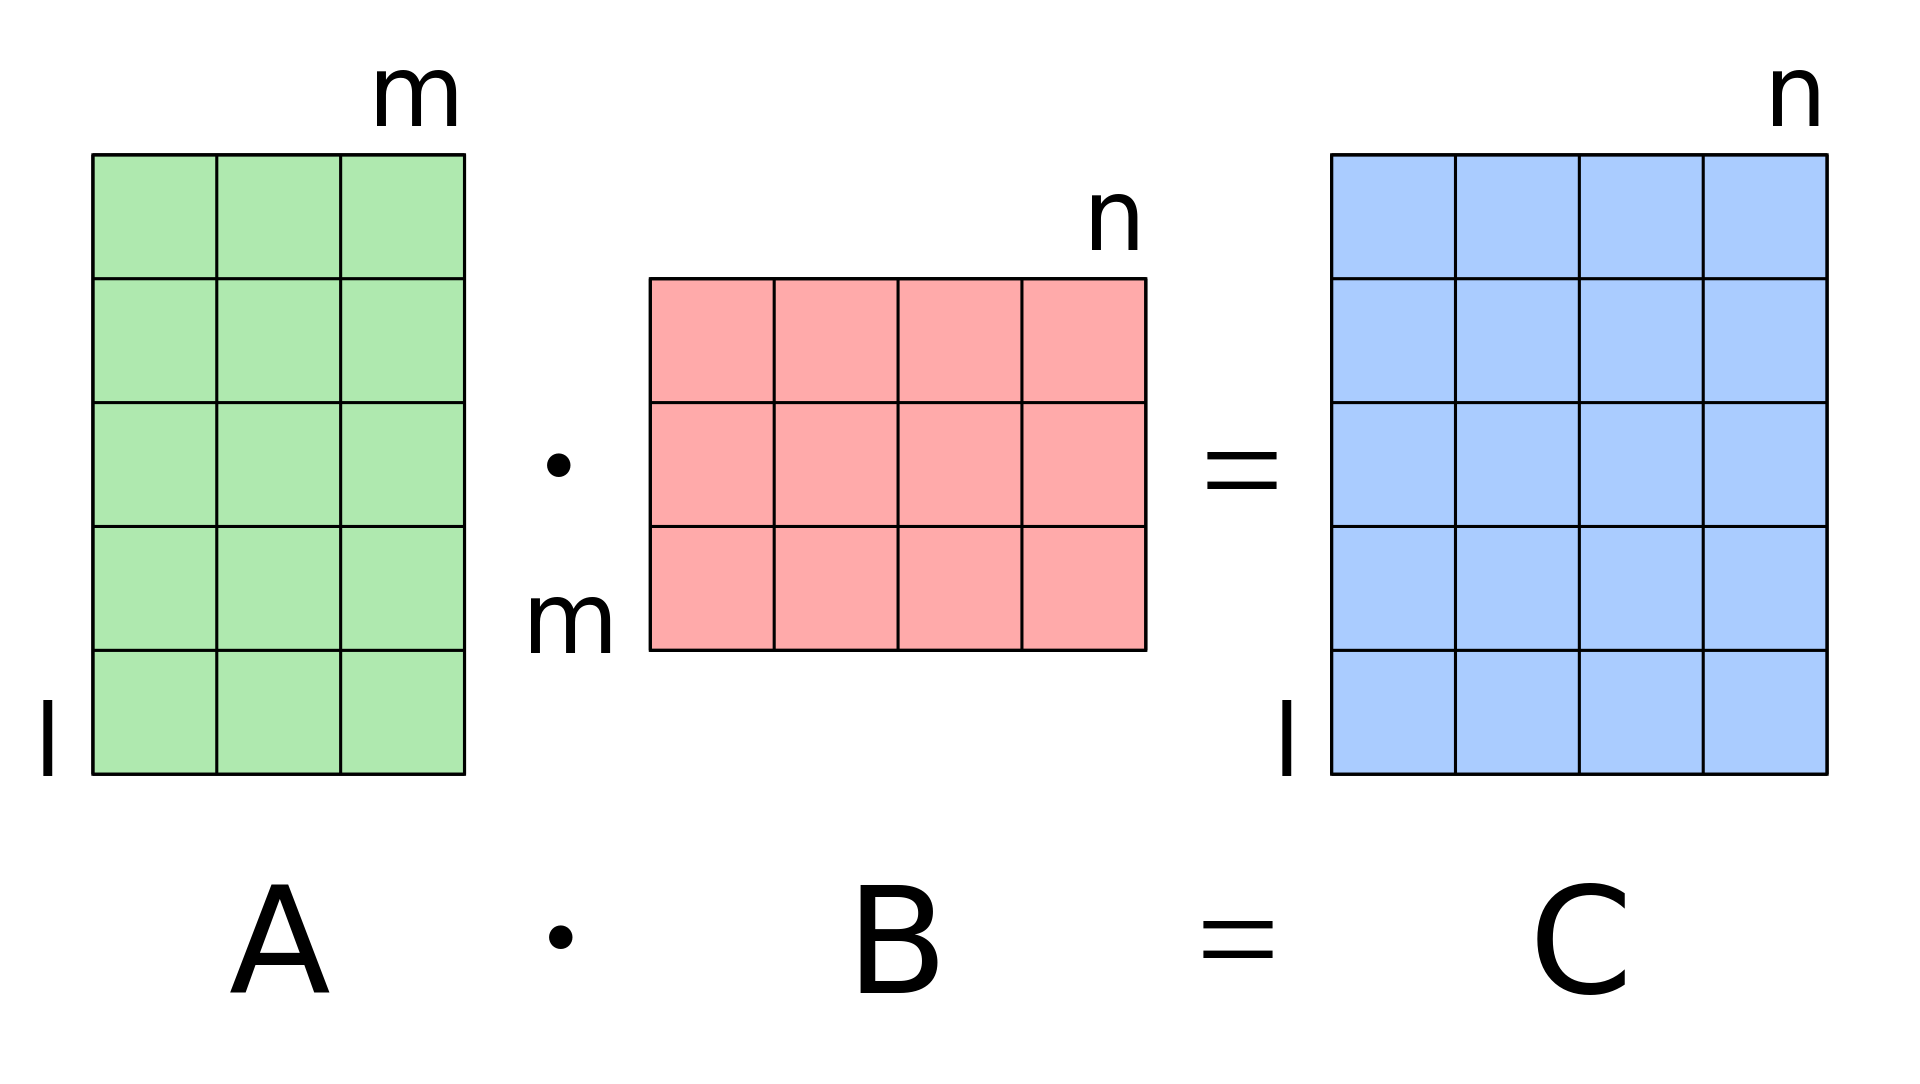
\includegraphics[width=0.5\textwidth,height=\textheight]{diplomka obrazky/4a.png}

\end{center}

Pri násobení matice skalárom, aka. jedným číslom, použijeme ako operátor
klasickú hviezdičku. Každý prvok matice bude prenásobený určeným číslom.

\begin{Shaded}
\begin{Highlighting}[]
\NormalTok{matica_riadky }\OperatorTok{*}\StringTok{ }\DecValTok{5}
\end{Highlighting}
\end{Shaded}

\begin{verbatim}
##         [,1] [,2] [,3]
## vektor1    5   10   15
## vektor2   20   25   30
## vektor3   35   40   45
\end{verbatim}

~

Pri násobení dvoch matíc sa používa trocha netradičný operátor
\(\%*\%\).

\begin{Shaded}
\begin{Highlighting}[]
\NormalTok{matica_riadky }\OperatorTok\StringTok{ }\NormalTok{matica_stlpce}
\end{Highlighting}
\end{Shaded}

\begin{verbatim}
##         vektor1 vektor2 vektor3
## vektor1      14      32      50
## vektor2      32      77     122
## vektor3      50     122     194
\end{verbatim}

~

Sčítanie matíc.

\begin{Shaded}
\begin{Highlighting}[]
\NormalTok{matica_riadky }\OperatorTok{+}\StringTok{ }\NormalTok{matica_stlpce}
\end{Highlighting}
\end{Shaded}

\begin{verbatim}
##         [,1] [,2] [,3]
## vektor1    2    6   10
## vektor2    6   10   14
## vektor3   10   14   18
\end{verbatim}

\hypertarget{transpozuxedcia-matice}{%
\subsubsection{Transpozícia matice}\label{transpozuxedcia-matice}}

Transponovaním matice dôjde k vzájomnej výmene riadkov a stĺpcov matice.
Takúto maticu označujeme ako \(A^T\). Ak bola prvotná matica \((m, n)\),
po transpozícií vznikne matica s rozmermi \((n, m)\). V R-ku matice
transponujeme pomocou funkcie \(t()\) ako \(transpose\).

\begin{Shaded}
\begin{Highlighting}[]
\NormalTok{matica_riadky}
\end{Highlighting}
\end{Shaded}

\begin{verbatim}
##         [,1] [,2] [,3]
## vektor1    1    2    3
## vektor2    4    5    6
## vektor3    7    8    9
\end{verbatim}

\begin{Shaded}
\begin{Highlighting}[]
\KeywordTok{t}\NormalTok{(matica_riadky)}
\end{Highlighting}
\end{Shaded}

\begin{verbatim}
##      vektor1 vektor2 vektor3
## [1,]       1       4       7
## [2,]       2       5       8
## [3,]       3       6       9
\end{verbatim}

\hypertarget{hodnosux165-rank-matice}{%
\subsubsection{Hodnosť (rank) matice}\label{hodnosux165-rank-matice}}

V zadaniach od vás bude požadované vyrátať hodnosť matice, čo sa zvykne
označovať aj ako rank matice. Hodnosť matice je maximálny počet lineárne
nezávislých riadkov, alebo stĺpcov, v matici. Dva vektory
\(\overrightarrow{\text{a}}\), \(\overrightarrow{\text{b}}\) nazývame
lineárne závislé vektory práve vtedy, ak existuje reálne číslo \(k\)
také, že platí:

\[\overrightarrow{b} = k\overrightarrow{a}\]

Ak táto rovnosť neplatí, vektory sú lineárne nezávislé. Keď sme
spomínali maximálny počet buď riadkov alebo stĺpcov, mysleli sme tým, že
ak nepracujeme so štvorcovou maticou, maximálna hodnosť môže byť najviac
rovná tomu, čoho je menej. Ak máme maticu 3x4, jej maximálna hodnosť
môže byť 3. Lebo riadkov máme menej. Ak by sme mali maticu 4x2,
maximálna hodnosť môže byť 2. Hodnosť matice sa v R-ku vyráta pomocou
funkcie \(qr()\).

\begin{Shaded}
\begin{Highlighting}[]
\CommentTok{# Predpokladajme, že pracujeme so štvorcovou maticou.}
\CommentTok{# Ak by ste mali overiť, či sú vektory lineárne nezávislé,}
\CommentTok{# všetky ich spojíme do matice, a vyrátame rank matice. Ak bude rank}
\CommentTok{# rovný počtu vektorov, vektory sú navzájom  lineárne nezávislé.}

\NormalTok{vektor1 <-}\StringTok{ }\KeywordTok{c}\NormalTok{(}\DecValTok{2}\NormalTok{, }\DecValTok{3}\NormalTok{, }\DecValTok{1}\NormalTok{, }\DecValTok{9}\NormalTok{)}
\NormalTok{vektor2 <-}\StringTok{ }\KeywordTok{c}\NormalTok{(}\DecValTok{1}\NormalTok{, }\DecValTok{0}\NormalTok{, }\DecValTok{3}\NormalTok{, }\DecValTok{4}\NormalTok{)}
\NormalTok{vektor3 <-}\StringTok{ }\KeywordTok{c}\NormalTok{(}\DecValTok{2}\NormalTok{, }\DecValTok{9}\NormalTok{, }\DecValTok{0}\NormalTok{, }\DecValTok{3}\NormalTok{)}
\NormalTok{vektor4 <-}\StringTok{ }\KeywordTok{c}\NormalTok{(}\DecValTok{4}\NormalTok{, }\DecValTok{7}\NormalTok{, }\DecValTok{2}\NormalTok{, }\DecValTok{4}\NormalTok{)}

\NormalTok{matica <-}\StringTok{ }\KeywordTok{rbind}\NormalTok{(vektor1, vektor2, vektor3, vektor4)}


\CommentTok{# Operátor "$" dokáže extrahovať konkrétnu hodnotu, ktorú chceme extrahovať. Skúste použiť}
\CommentTok{# príkaz "qr(matica)", ktorý nám vyráta ešte pár ďalších vecí. Nás však zaujíma iba rank.}

\KeywordTok{qr}\NormalTok{(matica)}\OperatorTok{$}\NormalTok{rank }\CommentTok{# vyrátame hodnosť matice}
\end{Highlighting}
\end{Shaded}

\begin{verbatim}
## [1] 4
\end{verbatim}

\begin{Shaded}
\begin{Highlighting}[]
\CommentTok{# Vidíme, že rank je rovný počtu riadkov/stĺpcov, teda naše vektory sú lineárne nezávislé.}
\end{Highlighting}
\end{Shaded}

\hypertarget{determinant-matice}{%
\subsubsection{Determinant matice}\label{determinant-matice}}

Determinant matice si môžeme predstaviť ako hodnotu, ktorá je priradená
matici podľa toho, ako vyzerá. Matice môžu mať determinant nulový alebo
nenulový. Mohli by sme to rátať ručne, necháme to však R-ko vyrátať za
nás. Nás budú zaujímať aké vlastnosti sa s determinantom spájajú.

\hypertarget{inverznuxe1-matica}{%
\subsubsection{Inverzná matica}\label{inverznuxe1-matica}}

Inverzná matica je matica \(A^{-1}\), ktorá nám po vynásobení pôvodnou
maticou A, dá jednotkovú maticu. Funguje to aj naopak, teda platí vzťah:

\[A * A^{-1} = A^{-1} * A = E\]

Inverznú maticu vytvoríme pomocou funkcie \(solve()\)

\hypertarget{singuluxe1rna-reguluxe1rna-matica}{%
\subsubsection{Singulárna / Regulárna
matica}\label{singuluxe1rna-reguluxe1rna-matica}}

Ak je matica regulárna, znamená to, že má inverziu. Ak je singulárna,
nemá inverziu, teda \(A^{-1}\) neexistuje.

\begin{itemize}
\tightlist
\item
  Matica je singulárna ak:

  \begin{itemize}
  \tightlist
  \item
    má determinant rovný nule,
  \item
    sa hodnost nerovná poctu riadkov (ak má napr. 3x3 matica hodnost 2)
  \end{itemize}
\item
  Matica je regulárna ak:

  \begin{itemize}
  \tightlist
  \item
    má nenulový determinant,
  \item
    sa hodnost rovná poctu riadkov/stlpcov.
  \end{itemize}
\end{itemize}

\hypertarget{pruxe1ca-s-datasetmi-a-ich-analuxfdza}{%
\section{Práca s datasetmi a ich
analýza}\label{pruxe1ca-s-datasetmi-a-ich-analuxfdza}}

Vrhneme sa na:

\begin{itemize}
\tightlist
\item
  načítanie datasetov do R-ka a objektov,
\item
  manipuláciu datasetov,
\item
  vysvetlenie lineárneho regresného modelu,
\item
  prácu s regresnými modelmi.
\end{itemize}

\hypertarget{naux10duxedtanie-duxe1t}{%
\subsection{Načítanie dát}\label{naux10duxedtanie-duxe1t}}

Načítať dáta je možné rôznymi spôsobmi. V okne \(Environment\) môžete
kliknúť na \(Import \ dataset\) a vybrať typ súboru, aký chcete
importovať. Sofistikovanejšie je však načítavanie údajov pomocou
funkcií. Tých je tiež niekoľko, plus, existujú rôzne balíky, ktoré sú
vyvinuté na zlepšenie práce s dátami a ich vizáže. Vám však bude stačíť
jediná funkcia a to \(read.csv2\). Predtým než funkciu použijeme, si
však treba nastoliť isté štandardy. Ideálne je, aby ste mali vytvorenú
zložku, v ktorej budete mať všetky datasety (excelovské súbory) a pekne
oddelené zložky k cvičeniam. Nazývame to ``working directory'' AKA
pracovný adresár. Na zistenie, kde je Váš momentálny pracovný adresár
použijeme funkciu \(getwd()\) (get working directorty). Potrebujeme to
vedieť preto, lebo do funkcie \(read.csv2\) potrebujeme zadať argument
umiestnenia súboru. A je ľahšie zadať:

\begin{Shaded}
\begin{Highlighting}[]
\KeywordTok{read.csv2}\NormalTok{(}\StringTok{"udaje_o_pocte_kaciatok"}\NormalTok{)}

\CommentTok{# než}

\KeywordTok{read.csv2}\NormalTok{(}\StringTok{"C:/Desktop/MilanRozok/ekonometria/test/udaje_o_pocte_kaciatok.csv"}\NormalTok{)}
\end{Highlighting}
\end{Shaded}

Určenie nového adresára je možné urobiť pomocou \(setwd()\) (set working
directory), kde ako argument zadáme cestu do nového adresára, avšak,
jednoduchšie je kliknúť vľavo hore na:

\begin{center}

Session -\textgreater{} Set Working Directory -\textgreater{} Choose
directory,

\end{center}

a vybrať si adresár manuálne. Všetky datasety potom môžeme načítať
funkciou \(read.csv2()\) už len pomocou uvedenia názvu v úvodzovách, a
nemusíme uvádzať celú cestu umiestnenia súboru.

\hypertarget{read.csv2}{%
\subsubsection{read.csv2()}\label{read.csv2}}

Súbory typu .CSV znamenajú doslovne \(Comma-separated \ values\), teda
hodnoty oddelené čiarkami. Keď sa bavíme o formáte .CSV predstavte si
súbor, kde každá hodnota má svoj riadok, a každá premenná má svoj
stĺpec. Ako hodnoty sa chápe oddelenie stlpcov, teda stĺpce sú väčšinou
oddelené čiarkami. To je však taký teoretický prístup, v praxi môžu byť
tieto hodnoty oddelené aj inými spôsobmi. Hlavné však je pozerať na
koncovku súboru, resp. súbor (napr. z Excelu), uložiť ako .CSV súbor.
Funkcie \(read.csv()\) a \(read.csv2()\) robia to isté, jediné v čom sa
líšia je ich defaultné nastavenie. \(read.csv()\) ráta, že sa na
oddelenie desatinných miest používa bodka (čo je také americké), a
\(read.csv2()\), používa na oddelenie desatinných miest čiarku (čo je
také európske). To je dôvod, prečo primárne používame \(read.csv2()\).

\hypertarget{pruxe1ca-so-vstavanuxfdmi-datasetmi}{%
\subsubsection{Práca so vstavanými
datasetmi}\label{pruxe1ca-so-vstavanuxfdmi-datasetmi}}

R-ko obsahuje vstavané datasety, ktoré si môžeme všetky vypísať pomocou:

\begin{Shaded}
\begin{Highlighting}[]
\KeywordTok{data}\NormalTok{()}
\end{Highlighting}
\end{Shaded}

V tomto sprievodcovi budeme pracovať s dátami, ktoré si môžete načítať
zo vstavaného balíka \(datasets\). Je to z dôvodu, že je to proste
jednoduché. Na hodinách budete pracovať s pravými ekonomickými
datasetmi, avšak pre ukážku, ako čo funguje, a ako s čím súvisí nám
postačia základné datasety, ktoré sú ľahké na pochopenie. Ak si budete
chcieť overiť nejakú funkciu či teóriu, budete si môcť za pochodu
načítať dataset, s ktorým ste oboznámený, a otestovať, čo potrebujete.

\begin{Shaded}
\begin{Highlighting}[]
\CommentTok{# Pre načítanie datasetu do objektu použijeme trocha nezvyčajný prístup, kde:}
\CommentTok{# datasets predstavuje názov balíku, a "mtcars" dataset, ktorý chceme sprístupniť.}
\CommentTok{# Pomocou "::" sprístupníme konkrétny objekt z balíka.}

\NormalTok{data <-}\StringTok{ }\NormalTok{datasets}\OperatorTok{::}\NormalTok{mtcars}

\CommentTok{# Ak by sme datasetu nechceli priradiť vlastný názov, ale ponechať originálny:}

\KeywordTok{data}\NormalTok{(}\StringTok{"mtcars"}\NormalTok{)}

\CommentTok{# Funkcia bude fungovať aj bez úvodzoviek.}
\end{Highlighting}
\end{Shaded}

\hypertarget{jednoduchuxe1-lineuxe1rna-regresia}{%
\section{Jednoduchá lineárna
regresia}\label{jednoduchuxe1-lineuxe1rna-regresia}}

Hlavným nástrojom ekonometrie je regresia. Cieľom regresie je zistiť ako
určená/é nezávislé premenné, ovplyvňujú jednu závislú premennú. Ak \(Y\)
je závislá a \(X\) nezávislá, tak regresujeme, robíme regresiu, Y na X.
Čo však tá magická skrinka vlastne robí?

\begin{Shaded}
\begin{Highlighting}[]
\CommentTok{# Predpokladajme, že máme načítaný dataset "mtcars".}
\CommentTok{# Pomocou funkcie "head()" si načítame prvých 6 riadkov.}
\CommentTok{# Alternatíva je "tail()" (ako chvost), pre vypísanie posledných 6 riadkov.}

\KeywordTok{head}\NormalTok{(data)}
\end{Highlighting}
\end{Shaded}

\begin{verbatim}
##                    mpg cyl disp  hp drat    wt  qsec vs am gear carb
## Mazda RX4         21.0   6  160 110 3.90 2.620 16.46  0  1    4    4
## Mazda RX4 Wag     21.0   6  160 110 3.90 2.875 17.02  0  1    4    4
## Datsun 710        22.8   4  108  93 3.85 2.320 18.61  1  1    4    1
## Hornet 4 Drive    21.4   6  258 110 3.08 3.215 19.44  1  0    3    1
## Hornet Sportabout 18.7   8  360 175 3.15 3.440 17.02  0  0    3    2
## Valiant           18.1   6  225 105 2.76 3.460 20.22  1  0    3    1
\end{verbatim}

\begin{Shaded}
\begin{Highlighting}[]
\CommentTok{# Vidíme, že je to súbor aút, s rôznymi parametrami.}
\CommentTok{# My sa budeme snažiť vysvetliť vplyv "hp" (horsepower, konské sily), }
\CommentTok{# na "mph" (miles per galon, čiže koľko kilometrov má auto dojazd).}
\end{Highlighting}
\end{Shaded}

Pozrime sa na tento model:

\[y_i = \beta_0 + \beta{x_i} + \epsilon_i.\]

Jedná sa o základný model lineárnej regresie. Ak si bety predstavíme ako
obyčajné hodnoty, model v tomto jednoduchom znení by Vám z matematiky
mohol byť povedomý. Výsledkom modelu je priamka \(y\), kde \(\beta_0\)
je obyčajná hodnota v ktorej je os Y pretnutá, \(\beta_1\) určuje sklon
priamky. Keďže priamka nebude prechádzať každou nameranou hodnotou,
\(\epsilon\) v modeli znázorňuje tento priestor medzi meraniami a
priamkou. Označujeme ho ako náhodnú zložku. Môže byť spôsobená mnohými
spôsobmi. Okrem iného napríklad: chybným meraním, náhodou, alebo
premennými, ktoré sme do modelu nezahrnuli. Jedno auto so 150 koňskými
silami môže na plnú nádrž prejsť 500km a druhé len 350. Môže to byť
spôsobené váhou, avšak v modeli máme len výkon auta. Táto zložka sa v
priemere rovná nule, a z modelu nám odpadne (viac o tom neskôr). Tento
model si môžeme v našom príklade prepísať ako:

\[mpg_i = \beta_0 + \beta_1{hp_i} + \epsilon_i.\] Priamka, ktorá by
vznikla výsledkom tohto modelu sa nazýva populačná regresná priamka. Na
vyhodnotenie takéhoto modelu by sme však potrebovali dáta z celej
určenej populácie, čo je veľmi často prakticky nemožné. Vo všeobecnosti
sú populačné parametre \(\beta_0\) a \(\beta_1\) neznáme. Avšak dokážeme
ich odhadnúť pomocou estimátorov. Preto pracujeme so vzorkami, ktoré
dokážeme reálne odpozorovať a zozbierať. Estimátory zo vzorky dokážu
poskytnúť dostatočne dôveryhodné odhady koeficientu v populácií. Poďme
si to teda ukázať na našej vzorke.

Skúsme si hodiť do grafu výkon a dojazd, nech sa pozrieme na vzťah medzi
týmito premennými.

\begin{Shaded}
\begin{Highlighting}[]
\CommentTok{# Plotneme si dáta, ktoré dáme do regresie, čiže "mpg" a "hp".}

\KeywordTok{plot}\NormalTok{(}\DataTypeTok{x =}\NormalTok{ data}\OperatorTok{$}\NormalTok{hp, }\DataTypeTok{y =}\NormalTok{ data}\OperatorTok{$}\NormalTok{mpg, }\DataTypeTok{ylab =} \StringTok{"ylab ako y label"}\NormalTok{, }\DataTypeTok{xlab =} \StringTok{"tu máme výkon",}
\StringTok{     main = "}\NormalTok{Vzťah dojazdu a výkonu motora}\StringTok{")}
\end{Highlighting}
\end{Shaded}

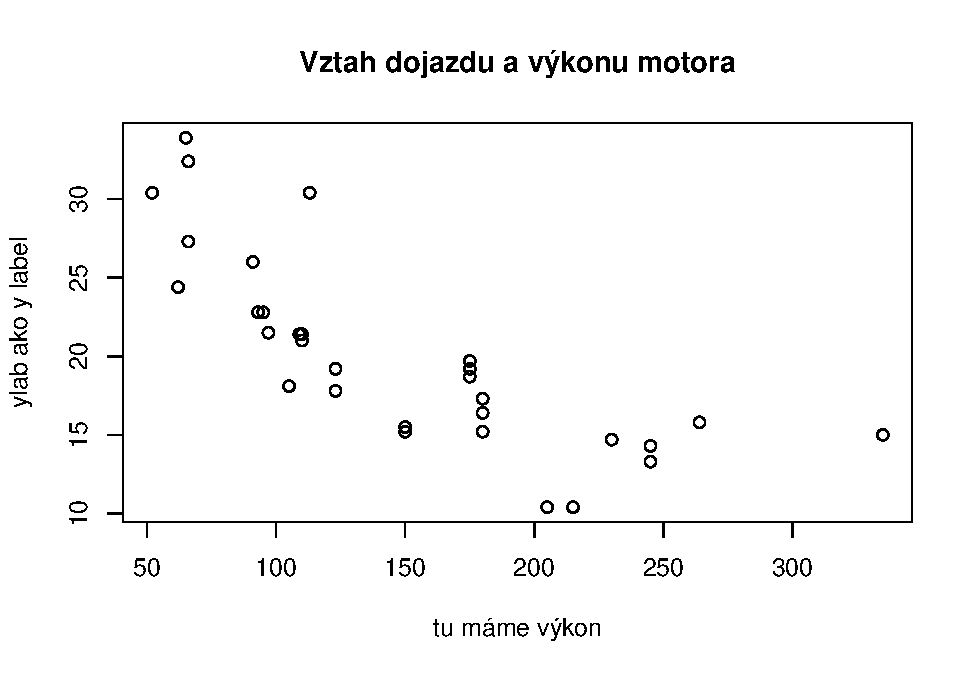
\includegraphics{test_files/figure-latex/unnamed-chunk-39-1.pdf}

Vidíme istú negatívnu závislosť. Chceli by sme si to však potvrdiť
číslami. Bolo by fajn napasovať medzi tieto pozorovania takú priamku,
ktorá bude ku každému pozorovaniu čo najbližšie. Keďže nepoznáme
parametre populácie, budeme pracovať s ich estimátormi, odhadcami.
Estimátory označíme striežkou ako \(\hat\beta_0{}\) a \(\hat\beta_1{}\).
Model bude vyzerať následovne:

\[\hat{mpg_i} = \hat\beta_0 + \hat \beta_1{hp_i}.\] \textgreater{}
\textbf{Náhodná zložka (error term) vypadne, lebo jej očakávaná hodnota
sa rovná nule.}

Skúsme si takýto model zostrojiť v R-ku, a priamku dopasovať do grafu.

\begin{Shaded}
\begin{Highlighting}[]
\CommentTok{# Chceme zistiť dopad "hp" na "mpg".}
\CommentTok{# Použijeme funkciu "lm()", ako linear model.}
\CommentTok{# Na konci musíme ako argument uviesť dáta, ktoré použijeme.}

\NormalTok{model <-}\StringTok{ }\KeywordTok{lm}\NormalTok{(mpg }\OperatorTok{~}\StringTok{ }\NormalTok{hp, }\DataTypeTok{data =}\NormalTok{ data)}

\CommentTok{# Alternatívne môžeme model napísať pomocou extrakcie takto.}
\CommentTok{# Preferujem tento postup.}

\NormalTok{model <-}\StringTok{ }\KeywordTok{lm}\NormalTok{(data}\OperatorTok{$}\NormalTok{mpg }\OperatorTok{~}\StringTok{ }\NormalTok{data}\OperatorTok{$}\NormalTok{hp)}

\CommentTok{# Dostaneme dva koeficienty. Jeden pre intercept Beta0 a druhý pre Beta1 ako "hp".}

\NormalTok{model}
\end{Highlighting}
\end{Shaded}

\begin{verbatim}
## 
## Call:
## lm(formula = data$mpg ~ data$hp)
## 
## Coefficients:
## (Intercept)      data$hp  
##    30.09886     -0.06823
\end{verbatim}

\begin{Shaded}
\begin{Highlighting}[]
\CommentTok{# Intercept sa väčšinou neinterpretuje, slúži len pre určenie počiatočnej hodnoty.}
\CommentTok{# Ak by sme koeficient interpretovali, mohli by sme povedať, že auto s nula koňmi}
\CommentTok{# prejde 30 míľ na galón. Koeficient B1 by sme interpretovali ako:}
\CommentTok{# "každá extra konská sila, zníži dojazd o -0.068 míle". }
\end{Highlighting}
\end{Shaded}

\begin{Shaded}
\begin{Highlighting}[]
\CommentTok{# Znova si plotneme dáta.}

\KeywordTok{plot}\NormalTok{(}\DataTypeTok{x =}\NormalTok{ data}\OperatorTok{$}\NormalTok{hp, }\DataTypeTok{y =}\NormalTok{ data}\OperatorTok{$}\NormalTok{mpg, }\DataTypeTok{ylab =} \StringTok{"Dojazd"}\NormalTok{, }\DataTypeTok{xlab =} \StringTok{"Výkon",}
\StringTok{     main = "}\NormalTok{Vzťah dojazdu a výkonu motora}\StringTok{")}

\StringTok{# A pomocou funkcie "}\KeywordTok{abline}\NormalTok{()}\StringTok{" napasujeme do grafu priamku modelu.}
\StringTok{# Abline ako priamka z bodu A do bodu B.}

\StringTok{abline(model) }
\end{Highlighting}
\end{Shaded}

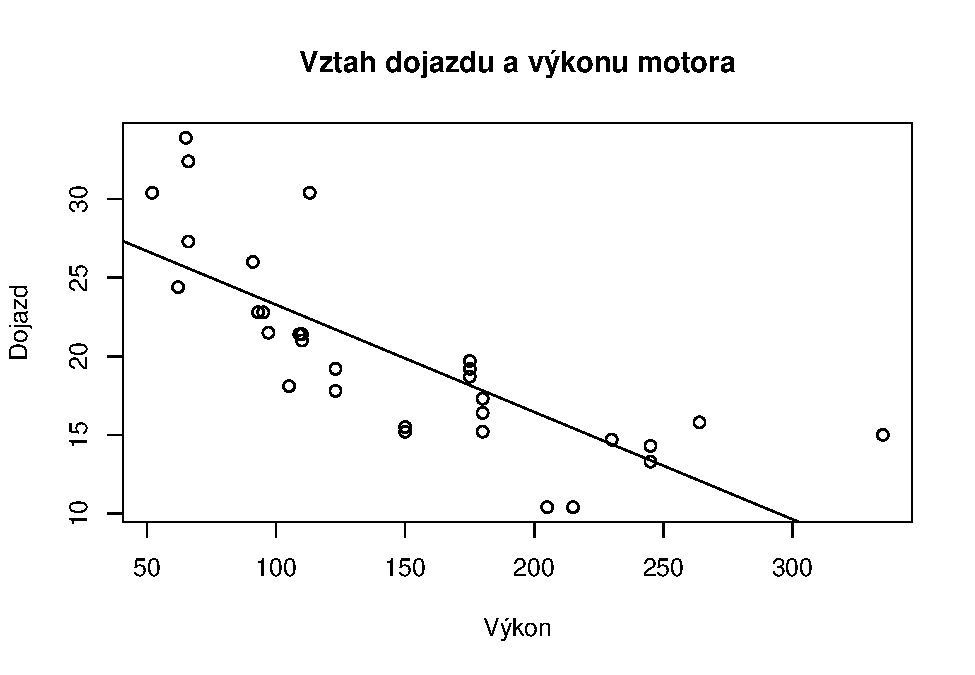
\includegraphics{test_files/figure-latex/unnamed-chunk-41-1.pdf}

Z grafu pozorujeme, že aj tu priamka neprechádza všetkými pozorovaniami,
túto kolmú vzdialenosť medzi priamkou a každým pozorovaním označíme ako
\(\hat{u}\). V tomto modeli to neoznačuje odhad náhodnej zložky
\(\epsilon\), ale výpočtovú nepresnosť modelu. Môžeme to brať ako takého
súrodenca k náhodnej zložke. Obe chyby predstavujú podobnú vec,
vzdialenosť medzi priamkou a pozorovaním. Priamku populácie je však
neznáma, teda aj táto vzdialenosť \(\epsilon\) je neznáma. Na druhú
stranu, zvyšky \(\hat{u}\) sú vyrátané z dát, a dokážeme ich presne
zmerať. Ako však vyrátame bety? Iste ste už začuli o OLS, teda Ordinary
Least Squares alebo Metódy najmenších štvorcov. Bety so striežkou
nazývame ako OLS estimátory. Metóda najmenších štvorcov sa to volá
preto, lebo vezmeme zvyšky \(\hat{u}\) z modelu, umocníme ich na druhú
mocninu (urobíme z nich štvorce), a minimalizujeme ich. Osobne si
nemyslím, že v tomto štádiu vašej výučby má veľký význam sústrediť sa na
odvodenie týchto estimátorov. Osobne mi to moc nedalo, preto sa skôr
zameriame na výsledky týchto odvodzovaní, nech nadobudneme trocha
intuície. Vysvetlíme si graficky, čo touto metódou chceme docieliť.

\begin{center}

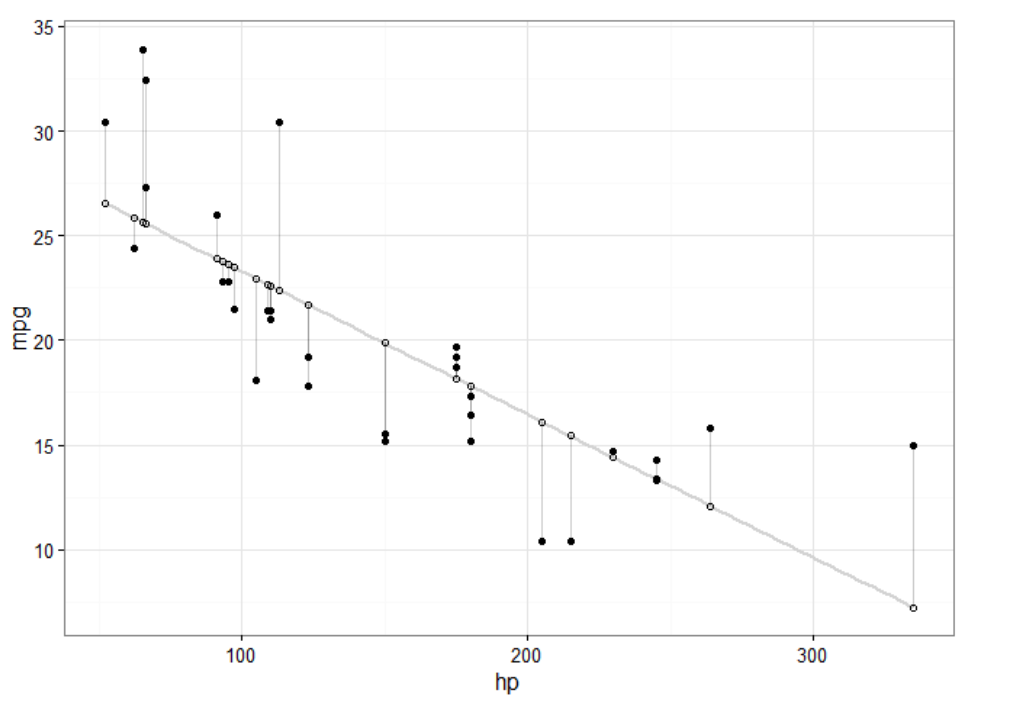
\includegraphics[width=0.85\textwidth,height=\textheight]{diplomka obrazky/4.png}

\end{center}

Tieto vzdialeností predstavujú naše ``residuals'' \(\hat{u}_i\), naše
zvyšky z modelu, naše nepresnosti. Každý data point má svoj zvyšok.
Logicky chceme, aby priamka čo najtesnejšie vystihovala dáta, chceme tým
pádom čo najviac zmenšiť zvyšky. Poďme sa k tým zvyškom dopracovať.

Pozorovanie sa rovná bodu na priamke \(\hat\beta_0 + \hat\beta{x}_i\)
plus zvyšok \(\hat{u}_i\):

\[ y_i = \hat\beta_0 + \hat\beta{x}_i + \hat{u}_i.\]

\begin{center}

Poprehadzujme si to, nech máme na jednej strane zvyšok \(\hat{u}_i\):

\end{center}

\[ \hat{u}_i = y_i - \hat\beta_0 - \hat\beta{x}_i.\]

Väčšinou narazíme na takýto zápis zvyškov, a to rozdiel medzi
pozorovanou hodnotou a odhadnutou hodnotou na priamke:

\[\hat{u}_i = y_i - \hat{y_i}.\]

\begin{center}

a keďže

\end{center}

\[ \hat{y}_i =\hat\beta_0 + \hat\beta{x}_i,\]

Tak sme tam, kde sme boli na začiatku, keď sme si dali zvyšok
\(\hat{u}_i\) na jednu stranu. OLS metóda urobí to, že minimalizuje
súčet našich umocnených zvyškov \(\hat{u}_i\):

\[min\sum (y_i - \hat\beta_0 - \hat\beta_1{x}_i)^2.\]

Tým, že minimalizujeme zvyšky dostaneme čo najlepšiu priamku, ktorá bude
sedieť čo najtesnejšie s dátami. Táto minimalizácia nám poskytne vzorec
na výpočet OLS estimátorov. Estimátorov parametrov populácie. Bavíme sa
o odhadcoch priesečníka, \(\beta_0\), a sklonu, \(\beta_1\). A keď sa
bavíme o odhadcoch, píšeme ich ako \(\hat\beta_0\) a \(\hat\beta_1\).
Nech si pamätáte.

Na hodinách sa stretnete so vzorcom pre výpočet biet v maticovej forme.
A to:

\[Est(\beta) = \hat\beta = (X^TX)^{-1}X^Ty.\]

\begin{quote}
\emph{T-čka znamenajú transpose matice a -1 vyrátanie inverzie.}
\end{quote}

\begin{Shaded}
\begin{Highlighting}[]
\CommentTok{# Inverznu maticu vyrátame pomocou "solve()" a transpozíciu pomocou "t()".}
\CommentTok{# V R-ku by sme to vyrátali ako:}

\KeywordTok{solve}\NormalTok{(}\KeywordTok{t}\NormalTok{(X) }\OperatorTok\StringTok{ }\NormalTok{X) }\OperatorTok\StringTok{ }\KeywordTok{t}\NormalTok{(X) }\OperatorTok\StringTok{ }\NormalTok{y}\ErrorTok{)}
\end{Highlighting}
\end{Shaded}

Tento vzorec by som nazval funkčným, avšak určite nie intuitívnym.
Pracujete s ním preto, lebo:

\begin{itemize}
\tightlist
\item
  takáto forma je ľahšie spracovateľná pre výpočtovú techniku,
\item
  R-ko pri práci s datasetom ho aj tak pretvorí na maticu, predtým než
  podá výsledky,
\item
  tento vzorec funguje ako pre jednoduchú lineárnu regresiu (jedno Y a
  jedno X), tak aj pre viacnásobnú regresiu (jedno Y a viacero X).
\end{itemize}

Ono, R-ko to urobí všetko za Vás, samo vyráta všetky koeficienty, nuž
nechceli by ste vedieť, čo tá \(\hat\beta\) vlastne robí? Pri
jednoduchej lineárnej regresií dokážeme OLS beta estimátory zapísať aj
takto:

\[\hat\beta_0 = \overline{y} - (\hat\beta_1\overline{x})\]

\[\hat\beta_1 = \frac{\sum_{i=1}^{n} (x_i - \overline{x})(y_i - \overline{y})}{\sum_{i=1}^{n} (x_i - \overline{x})^2}\]

\begin{quote}
\emph{Čiara nad písmenom znamená priemer, teda ybar(takto to čítame) je
priemer všetkých hodnôt ``y'' v datasete.}
\end{quote}

Neopúšťajte ma. Ak Vám tento vzorec nie je povedomý, nič sa nedeje.
Pozrieme sa na to. Rozdeľme si to na vrch a spodok. Začneme menovateľom,
lebo je kratší, hm.

Súčet od i = 1 po n znamená, že vykonáme operáciu pre každé \(x\) v
datasete a výsledky operácií sčítame.

\begin{quote}
\emph{Summation znak sa nazýva grécky sigma.}
\end{quote}

Od každého \(x\) odčítame priemernú hodnotu \(\overline{x}\) a umocníme
to. Získame tým variabilitu okolo priemeru, inak povedané, ako veľmi sú
data v datasete rozptýlené. Dostaneme rozptyl. Je dôležité podotknúť, že
rozptyl kvôli umocneniu nikdy nebude záporný. Dôležité je to preto, lebo
vzťah v čitateli určuje, či je \(\beta\) pozitívna alebo negatívna.
Takže menovateľ neovplyvní kladnosť či zápornosť čitateľa.

Vzťah v čitateli vyzerá celkom podobne k tomu v menovateli, hm? A nie je
to náhoda. Vzťah v čitateli je obyčajná kovariancia, inak povedané,
spoločný rozptyl. Predstavuje závislosť medzi dvoma veličinami. Tento
vzťah neumocňujeme, pretože chceme vidieť, či bude závislosť pozitívna,
alebo negatívna.

\begin{quote}
\emph{Kovariancia či korelácia? Čo je čo? Korelácia je štandardizovaná
kovariancia. Obe vysvetľujú to isté, líšia sa len v rozsahu. Kovarianciu
predelíme násobkom smerodajných odchýlok x a y, a získame koreláciu.
Štandardizujeme to preto, aby sme sa vedeli orientovať, aký veľký je v
skutočnosti vzťah medzi premennými. Ak sa bavíme o kovariancii hmotnosti
v kilogramoch a dĺžky lietadla v metroch, výsledné hodnoty budú veľmi
vysoké. Ak budú kladné, budeme vedieť, že je medzi nimi lineárna
závislosť, ale nevieme aká veľká. Ak by sme porovnávali kovarianciu
kurzu EUR a USD, výsledné hodnoty budú síce menšie, ale stále o nič viac
vhodné na interpretovanie. Ak však tieto hodnoty predelíme násobkom
smerodajných odchýlok, teda ich štandardizujeme, výsledné hodnoty budú
porovnateľné pre akékoľvek premenné. Keďže ťažké a dlhé lietadlo bude
mať úmerne veľké smerodajné odchýlky, kdežto výmenný kurz bude mať
smerodajnú odchýlku prislúchajúcu hodnotám kurzu. Hodnoty v korelácií
budú spadať medzi hranice -1 a 1. Kde záporná hodnota predstavuje
negatívnu lineárnu závislosť, a naopak.}
\end{quote}

Pri odhade však nechceme hodnoty štandardizovať, ale vecne odhadnúť
použiteľné hodnoty koeficientov. \(\hat\beta_1\) si jednoducho zapíšeme
ako:

\[\hat\beta_1 = \frac{Cov(x, y)}{Var(x)}.\] Otestujme si, či to naozaj
funguje.

\begin{Shaded}
\begin{Highlighting}[]
\CommentTok{# Pripomeňme si hodnoty nášho modelu.}

\NormalTok{model}
\end{Highlighting}
\end{Shaded}

\begin{verbatim}
## 
## Call:
## lm(formula = data$mpg ~ data$hp)
## 
## Coefficients:
## (Intercept)      data$hp  
##    30.09886     -0.06823
\end{verbatim}

\begin{Shaded}
\begin{Highlighting}[]
\CommentTok{# Na poradí pri kovariancii nezáleží.}

\NormalTok{kovar <-}\StringTok{ }\KeywordTok{cov}\NormalTok{(data}\OperatorTok{$}\NormalTok{mpg, data}\OperatorTok{$}\NormalTok{hp)}

\NormalTok{rozptyl <-}\StringTok{ }\KeywordTok{var}\NormalTok{(data}\OperatorTok{$}\NormalTok{hp)}

\NormalTok{beta1 <-}\StringTok{ }\NormalTok{kovar}\OperatorTok{/}\NormalTok{rozptyl}

\KeywordTok{print}\NormalTok{(beta1)}
\end{Highlighting}
\end{Shaded}

\begin{verbatim}
## [1] -0.06822828
\end{verbatim}

\begin{Shaded}
\begin{Highlighting}[]
\CommentTok{# Oba parametre majú hodnotu -0.068 a rovnajú sa.}
\CommentTok{# Skúsme B0.}

\NormalTok{ybar <-}\StringTok{ }\KeywordTok{mean}\NormalTok{(data}\OperatorTok{$}\NormalTok{mpg)}
\NormalTok{xbar <-}\StringTok{ }\KeywordTok{mean}\NormalTok{(data}\OperatorTok{$}\NormalTok{hp)}

\NormalTok{beta0 <-}\StringTok{ }\NormalTok{ybar }\OperatorTok{-}\StringTok{ }\NormalTok{(beta1 }\OperatorTok{*}\StringTok{ }\NormalTok{xbar)}

\KeywordTok{print}\NormalTok{(beta0)}
\end{Highlighting}
\end{Shaded}

\begin{verbatim}
## [1] 30.09886
\end{verbatim}

\begin{Shaded}
\begin{Highlighting}[]
\CommentTok{# Sedí. :)}
\end{Highlighting}
\end{Shaded}

Nevravím, že sme objavili Ameriku, ale aspoň viete, že \(\hat\beta_0\)
je nejaký priemer \(y\) a od toho odčítame \(\hat\beta_1\) vynásobenú
priemerom \(x\). A neskrýva sa za tým žiaden ťažký imaginárny vzorec.
Taktiež, že \(\hat\beta_1\) je spoločný rozptyl závislej a nezávislej
premennej, vydelený rozptylom nezávislej premennej.

Ako však vieme, či estimátorom \(\hat\beta_0\) a \(\hat\beta_1\) môžeme
veriť?

\hypertarget{trocha-ux161tatistiky}{%
\section{Trocha štatistiky}\label{trocha-ux161tatistiky}}

Predtým, než si povieme o podmienkach lineárnej regresie Vás oboznámim s
pár záležitosťami, s ktorými sa stretnete, a napriek tomu, že sú pomerne
jednoduché by Vám zabrali dosť googlenia.

Prejdeme si:

\begin{itemize}
\tightlist
\item
  normálne rozdelenie,
\item
  očakávanú hodnotu,
\item
  zákon veľkých čísel,
\item
  náhodný výber,
\item
  centrálnu limitnú vetu.
\end{itemize}

Možno ste si všimli, že pri interpretáciach koeficientov sa často
opakuje niečo v zmyysle:``V priemere nám pri zvýšeni bla bla bla
narastie o bla bla bla.'' To \textbf{v priemere} je veľmi podstatné.
Väčšinou pracujeme so vzorkami, ktoré boli zozbierané z populácie, ktorá
je pre nás neznáma. Ideálne boli vybrané náhodným výberom, čo spôsobí,
že pozorovania vo vzorke sú náhodnými veličinami, a štatistiky ktoré z
nich vyrátame sú taktiež náhodné veličiny. Prečo je to podstatné sa
dozvieme v nasledujúcich konceptoch.

\begin{quote}
\emph{Keď sa bavíme o štatistikách, máme na mysli akúkoľvek hodnotu,
ktorú je možné vyrátať a opisuje niečo. Priemer je štatistika, rozptyl
je štatistika."}
\end{quote}

\hypertarget{normuxe1lne-rozdelenie}{%
\subsection{Normálne rozdelenie}\label{normuxe1lne-rozdelenie}}

Je potrebné vedieť, ako toto rozdelenie vyzerá, a aké má vlastnosti,
keďže mnoho konceptov v štatistike, sa točí okolo tohto rozdelenia,
kvôli jeho sladkým vlastnostiam. Normálne rozdelenie je rozdelenie
pravdepodonosti, ktoré je symetrické okolo priemeru, čím znázorňuje, že
hodnoty okolo priemeru majú vyššiu pravdepodobnosť výskytu. V porovnaní
s dátami na chvoste rozdelenia. Normálne rozdelenie má dva parametre:

\begin{itemize}
\tightlist
\item
  priemer,
\item
  smerodajnú odchýlku.
\end{itemize}

Pre normálne rozdelenie platí, že 68\% pozorovaní je v rozmedzí 1
smerodajnej odchýlky (od priemeru na každú stranu jedna), 95\%
pozorovaní je v romedzí 2 smerdajných odchýlok a 99,7\% pozorovaní v
rozmedzí 3 smerodajných odchýlok. To sa nám zíde pri testovaní hypotéz.

\begin{Shaded}
\begin{Highlighting}[]
\CommentTok{# Zostrojme si pre ilustráciu normálne rozdelenie.}
\CommentTok{# Môžeme pôžiť dnorm(), pre vyrátanie krásneho normálneho rozdelenia, ktorému}
\CommentTok{# by sme zadali vlastné hodnoty, my však použijeme rnorm(), pre vygenerovanie}
\CommentTok{# n hodnôt z normálneho rozdelenia.}

\NormalTok{nrozdelenie <-}\StringTok{  }\KeywordTok{rnorm}\NormalTok{(}\DataTypeTok{n =} \DecValTok{1000}\NormalTok{, }\DataTypeTok{mean =} \DecValTok{20}\NormalTok{, }\DataTypeTok{sd =} \DecValTok{5}\NormalTok{)}

\CommentTok{# Použijeme hist() namiesto plot(). Funkcia plot() by defaultne použila scatterplot.}
\CommentTok{# Argument "breaks" určí, na koľko častí rozlámeme náš histogram.}
\CommentTok{# Viacej častí nám umožní krajšie vystihnúť normálne rozdelenie.}
\CommentTok{# Funkciou par() si zobrazíme dva grafy vedľa seba a ukážeme rozdiel.}

\KeywordTok{par}\NormalTok{(}\DataTypeTok{mfrow=}\KeywordTok{c}\NormalTok{(}\DecValTok{1}\NormalTok{, }\DecValTok{2}\NormalTok{)) }

\CommentTok{# Všimnime si, že sú centrované okolo priemeru, ktorý sme zadali ako 20.}

\KeywordTok{hist}\NormalTok{(nrozdelenie, }\DataTypeTok{breaks =} \DecValTok{10}\NormalTok{, }\DataTypeTok{main =} \StringTok{"10 breakov"}\NormalTok{)}

\KeywordTok{hist}\NormalTok{(nrozdelenie, }\DataTypeTok{breaks =} \DecValTok{30}\NormalTok{, }\DataTypeTok{main =} \StringTok{"30 breakov"}\NormalTok{)}
\end{Highlighting}
\end{Shaded}

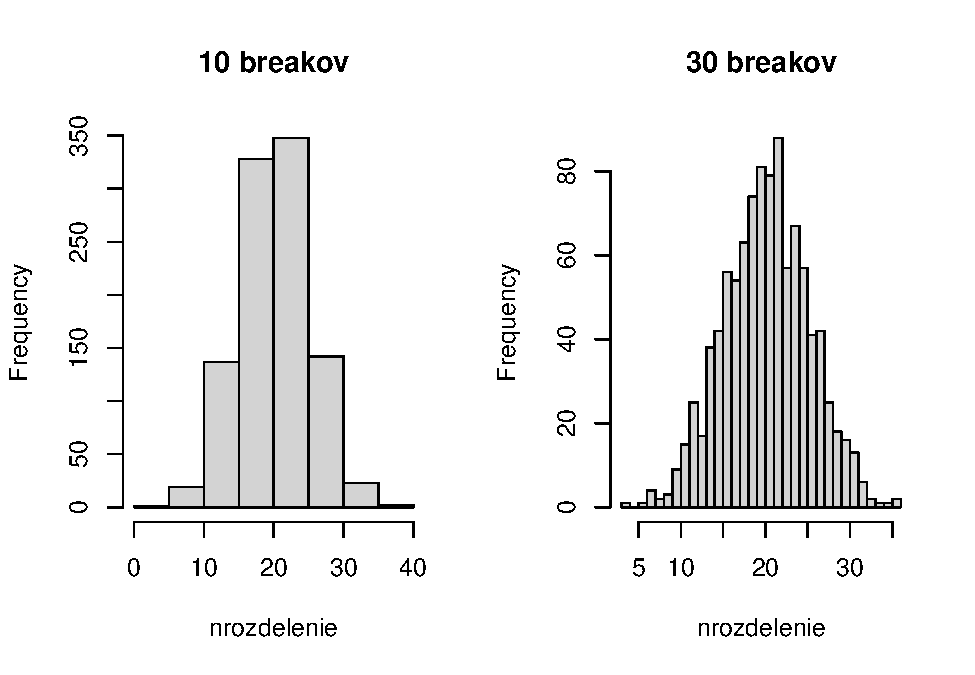
\includegraphics{test_files/figure-latex/unnamed-chunk-44-1.pdf}

\begin{Shaded}
\begin{Highlighting}[]
\CommentTok{# Pre navrátenie zobrazenia grafov na jeden, použijeme "par(mfrow=c(1, 1))".}
\end{Highlighting}
\end{Shaded}

\hypertarget{oux10dakuxe1vanuxe1-hodnota}{%
\subsection{Očakávaná hodnota}\label{oux10dakuxe1vanuxe1-hodnota}}

Spomínam si, ako som otvoril videa Bena Lamberta, a tam na mňa vyskočilo
hneď nejaké tlačené É-čko a rôzne kvačky. Veľké tlačené E znamená
expected value, teda očakávaná hodnota. Je to tak, ako to znie.
Očakávaná hodnota náhodnej premennej je jednoducho povedané priemer,
ktorý by sme vyrátali za dlhú dobu a pri niekoľkonásobnom opakovanom
výbere vzorky. Pre diskrétnu náhodnú premennú vyrátame túto hodnotu ako
vážený súčet, kde váha je určená pravdepodobnosťou výskytu. Vzorcom:

\[E(y)= y_1p_1 + y_2p_2 + ... + y_kp_k = \sum_{i=1}^{k}y_ip_i\]

A teraz príklad zo života na pochopenie. Prečo myslíte, sa hovorí
``Lucky Seven'', teda že sedmička je šťastné číslo? Je to preto, lebo
keď sčítate všetky kombinácie čísel na dvoch hracích kockách, najviac
hodnôt vyjde pre 7, teda aj pravdepodobnosť, že padne toto číslo je
väčšia, ako pri ostatných súčtoch. V priemere potom padne najviac ľudom
sedmička, ľudia si to všímajú a stavujú na sedmičky, alebo také niečo,
nie som moc na gambling.

\begin{center}

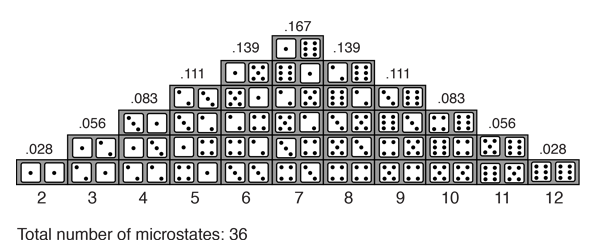
\includegraphics[width=0.8\textwidth,height=\textheight]{diplomka obrazky/5.png}

\end{center}

\hypertarget{zuxe1kon-veux13ekuxfdch-ux10duxedsel}{%
\subsection{Zákon veľkých
čísel}\label{zuxe1kon-veux13ekuxfdch-ux10duxedsel}}

S tým úzko súvisí aj zákon veľkých čísel. Zákon vraví, že ak rovnaký
experiment opakujeme nezávisle od seba nespočetne veľa krát, priemer
výsledkov bude blízko k \textbf{očakávanej hodnote}. Výsledok sa bude
približovať k očakávanej hodnote, ako sa bude počet pokusov zvyšovať.

\emph{Príklad:} Keď si s niekym budete hádzať mincu, možno padne 10-krát
za sebou orol, ale keby sme mincu hodili miliónkrát, výsledky by boli
približne 50/50. Inak povedané, šanca že padne hlava (alebo orol) je
50\%, ak minca nie je cinknutá. Očakávaná hodnota pri hode mincou je
0.5. Šanca že padne hlava je 1 a možné výsledky sú 2, teda
pravedpodobnosť, že padne hlava je 0.5, čiže 50\%.

\hypertarget{nuxe1hodnuxfd-vuxfdber}{%
\subsection{Náhodný výber}\label{nuxe1hodnuxfd-vuxfdber}}

V angličtine random sampling. To ing značí nejakú činnosť. Náhodný výber
znie skôr ako jeden výber, avšak pri random sampling ide o niečo iné.
Väčšina ekonometrických procedúr pracuje s priemermi vzoriek. Čiže tento
náhodný výber, sa bude týkať priemeru. Povedzme, že chceme odhadnúť
priemernú výšku v populácií. Väčšinou predpokladáme, že pozorovania sú
zozbierané náhodne z veľkej, nepoznanej populácie. Vyrátanie priemeru z
takejto vzorky má za následok to, že tento priemer je \emph{náhodnou
premennou}. \emph{Táto náhodná premenná má potom rozdelenie
pravdepodobnosti, nazývané výberové rozdelenie.} Výberové rozdelenie
závisí od rozdelenia populácie, z ktorej sme vzorku zobrali.
Predpokladajme, že máme normálne distribuovanú populáciu, a vyberieme z
nej veľa veľa vzoriek, vyrátame priemer týchto vzoriek, a urobíme z
týchto priemerov histogram. Rozdelenie tohto histogramu bude kopírovať
rozdelenie, z ktorého sme tieto vzorky zobrali, teda normálne
rozdelenie. Náhodný výber by mal eliminovať odchýlku, keďže každý z
populácie má rovnakú šancu byť vybraný. Získame teda rozdelenie bez
odchýlky, ktoré kopíruje rozdelenie populácie. Hlavným trikom tohto
náhodného výberu je, že jeho rozdelenie môže byť blízko normálneho
rozdelenia, aj keď populácia z ktorej sme brali vzorky nemá normálne
rozdelenie. A to vďaka Centrálnej limitnej vete.

\hypertarget{centruxe1lna-limitnuxe1-veta}{%
\subsection{Centrálna limitná veta}\label{centruxe1lna-limitnuxe1-veta}}

Kdežto Zákon veľkých čísel sa zameriaval skôr na odhad danej štatistiky,
Centrálna limitná veta súvisí s rozdelením vzorky. Podstatou je, že ak
vezmeme dostatočne veľké množstvo priemerov vzoriek, súbor týchto
priemerov bude mať normálne rozdelenie, bez ohľadu na rozdelenie
populácie. Takáto vzorka by mala mať aspoň 30 pozorovaní. Nie je však
potrebné zbierať veľa veľa vzoriek, keďže na vzorku použijeme estimátor,
napríklad na odhad priemeru, a samotný výsledok bude náhodná veličina
(ako sme už spomenuli pri náhodnom výbere), ktorá sama pochádza z
náhodného výberu. Čiže na splnenie predpokladu, že výsledné rozdelenie
budeme môcť odhadnúť normálnym rozdelením, závisí už len od veľkosti
vzorky. Čím vzdialenejšie od normálneho rozdelenia je rozdelenie
populácie, tým väčšia vzorka bude potrebná, aby toto pravidlo platilo.

\hypertarget{podmienky-lineuxe1rnej-regresie}{%
\section{Podmienky lineárnej
regresie}\label{podmienky-lineuxe1rnej-regresie}}

Prečo som Vám toto všetko vravel? Pracujeme s náhodnými veličinami,
takže pochopiť zmysel náhodného výberu, je dôležité. Všetky estimátory s
ktorými pracujeme, teda \(\hat\beta{}_i\), sú náhodnými veličinami (lebo
sú vyrátané z náhodnej vzorky), teda na ich vyrátané koeficienty budú
platiť vyššie spomínané koncepty. Keď budeme pracovať s predpokladom, že
majú normálne rozdelenie, môžeme na nich aplikovať t-testy a konfidenčné
intervaly a ďalšie krásne štatistické techniky. Tento predpoklad môžeme
použiť vďaka očakávanej hodnote, keďže:

\[E(\overline{x}) = \mu\] Teda očakávaná hodnota nášho estimátora (v
tomto prípade je priemer vzorky estimátor priemeru populácie) bude rovná
priemeru populácie mí. Ono, sú to také štatistické kecy, ktoré majú
svoje opodstatnenie, avšak potrebujete troška času, aby ste sa s nimi
vžili a pochopili ich. Týmto vzorcom chceme povedať, že predpokladáme,
že rozdelenie priemeru v našej vzorke nebude odchýlené od priemeru
populácie, lebo pri očakávanej hodnote by sme vzali nekonečno veľa
vzoriek, a platil by Zákon veľkých čísel a Centrálna limitná veta. A
naša vzorka je náhodne vybraná, tak predpokladáme, že má normálne
rozdelenie a môžeme s ňou podľa toho pracovať, a aplikovať na ňu
štatistické techniky.

\hypertarget{blue}{%
\subsection{BLUE}\label{blue}}

My chceme, aby naše estimátory boli BLUE! A tým nemyslíme modré, ale
Best Linear Unbiased Estimators! Najlepší Lineárni Nevychýlení
Odhadcovia! Unbiased znamená, že v priemere Beta trafí cieľ, teda
priemer populácie. A naše \(\beta_i\) estimátory spĺňajú tieto
požadované vlastnosti, ak sú splnené isté podmienky. Určite ste počuli o
Gauss-Markov podmienkach, po ktorých splnení sú OLS estimátory BLUE.
Niekto ich uvádza 5, niekto 10. Nebudeme si ich tu všetky preberať, lebo
nuda. Spomenieme si len pár. Všetky tieto štatistické veci som Vám
vysvetľoval preto, lebo jednou z podmienok je, že:

\begin{center}

\begin{quote}
\emph{Vzorka s ktorou model pracuje musí byť zozbieraná náhodne z
populácie.}
\end{quote}

\end{center}

To znamená, že vzorka by mala byť \(i.i.d\). Independently and
Identically Distributed. Nezávislo a identicky distribovaná. To znamená,
že výber jedného pozorovania zo vzorky, neovplyvňuje výber ďalšieho
pozorovania, a že každé pozorovanie má rovnakú šancu byť vybrané. Ak to
tak bude, naše estimátory budú nevychýlené. \emph{Kvôli konceptom, ktoré
sme si predstavili vyššie.}

\begin{Shaded}
\begin{Highlighting}[]
\CommentTok{# Ukážme si, čo to biased vlastné znamená. Použijeme na to dnorm().}
\CommentTok{# dnorm() nám vyberie konkrétny bod z rozdelenia, preto je potrebné mu zadať}
\CommentTok{# vektor.}

\NormalTok{x <-}\StringTok{ }\KeywordTok{seq}\NormalTok{(}\DataTypeTok{from =} \DecValTok{-3}\NormalTok{, }\DataTypeTok{to =} \DecValTok{5}\NormalTok{, }\DataTypeTok{by =} \FloatTok{0.2}\NormalTok{)}

\CommentTok{# type = "l" ako "line", čiara.}
\CommentTok{# Povedzme, že populačný priemer mí, je 1.}
\CommentTok{# Zaznačíme si ho v grafe pomocou abline(), použijeme arugment "v" ako vertical.}


\KeywordTok{plot}\NormalTok{(}\DataTypeTok{x =}\NormalTok{ x, }\DataTypeTok{y =} \KeywordTok{dnorm}\NormalTok{(x, }\DataTypeTok{mean =} \DecValTok{2}\NormalTok{, }\DataTypeTok{sd =} \DecValTok{1}\NormalTok{), }\DataTypeTok{type =} \StringTok{"l"}\NormalTok{,}
     \DataTypeTok{main =} \StringTok{"biased rozdelenie"}\NormalTok{, }\DataTypeTok{ylab =} \StringTok{""}\NormalTok{, }\DataTypeTok{xlab =} \StringTok{""}\NormalTok{)}

\KeywordTok{abline}\NormalTok{(}\DataTypeTok{v =} \DecValTok{1}\NormalTok{)}
\end{Highlighting}
\end{Shaded}

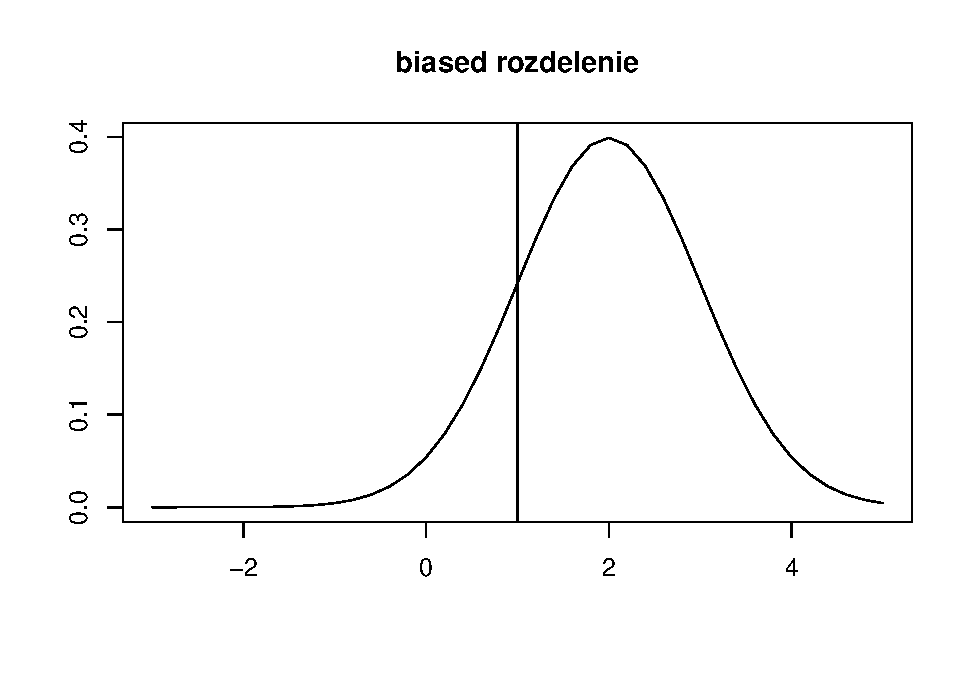
\includegraphics{test_files/figure-latex/unnamed-chunk-45-1.pdf}

Vrchol rozdelenia nie je centrovaný nad pravým priemerom, rozdelenie je
teda biased, odchýlené.

\textbf{Odchýlka však nie je jediná vec, ktorá by nás mala zaujímať.}
Potrebujeme taktiež overiť, či sú naše odhadnuté koeficienty
interpretovateľné a aplikovateľné na populáciu. K tomu nám dopomáha
štandardná chyba odhadnutých \(\hat\beta{}_i\)iet. Táto chyba je však
skreslená pri porušení ďalších Gauss-Markov podmienok. Tieto podmienky
sa týkajú chýb modelu (residuals \(\hat u_i\)). Prv sa však oboznámme s
tým, ako sú nám štandardné chyby nápomocné.

\hypertarget{vuxfdstup-regresie}{%
\section{Výstup regresie}\label{vuxfdstup-regresie}}

Pozrime sa na výstup našej regresie a analyzujme si ho troška.

\begin{Shaded}
\begin{Highlighting}[]
\CommentTok{# Na výpis všetkých vlastností modelu použijeme summary().}

\KeywordTok{summary}\NormalTok{(model)}
\end{Highlighting}
\end{Shaded}

\begin{verbatim}
## 
## Call:
## lm(formula = data$mpg ~ data$hp)
## 
## Residuals:
##     Min      1Q  Median      3Q     Max 
## -5.7121 -2.1122 -0.8854  1.5819  8.2360 
## 
## Coefficients:
##             Estimate Std. Error t value Pr(>|t|)    
## (Intercept) 30.09886    1.63392  18.421  < 2e-16 ***
## data$hp     -0.06823    0.01012  -6.742 1.79e-07 ***
## ---
## Signif. codes:  0 '***' 0.001 '**' 0.01 '*' 0.05 '.' 0.1 ' ' 1
## 
## Residual standard error: 3.863 on 30 degrees of freedom
## Multiple R-squared:  0.6024, Adjusted R-squared:  0.5892 
## F-statistic: 45.46 on 1 and 30 DF,  p-value: 1.788e-07
\end{verbatim}

\begin{Shaded}
\begin{Highlighting}[]
\CommentTok{# Vidíme tam nejaké vlastnosti reziduí, odhadnuté koeficienty, a v tretej}
\CommentTok{# časti taktiež podstatné veci ako R^2, či F-test.}
\CommentTok{# Teraz nás však zaujíma časť s koeficientmi.}

\KeywordTok{summary}\NormalTok{(model)}\OperatorTok{$}\NormalTok{coefficients}
\end{Highlighting}
\end{Shaded}

\begin{verbatim}
##                Estimate Std. Error   t value     Pr(>|t|)
## (Intercept) 30.09886054  1.6339210 18.421246 6.642736e-18
## data$hp     -0.06822828  0.0101193 -6.742389 1.787835e-07
\end{verbatim}

\hypertarget{t-test}{%
\subsection{t-test}\label{t-test}}

Na to, aby sme určili, či sú koeficienty významné, používame t-test. To,
čo vidíme v koeficientoch v stĺpci \(t\) je označované ako
\(t-štatistika\), lebo je to štatistickou technikou vyrátaná hodnota,
ktorá je interpretovateľná. Aaale prečo vlastne t-štatistika? Pozrime sa
na t-rozdelenie.

\begin{center}

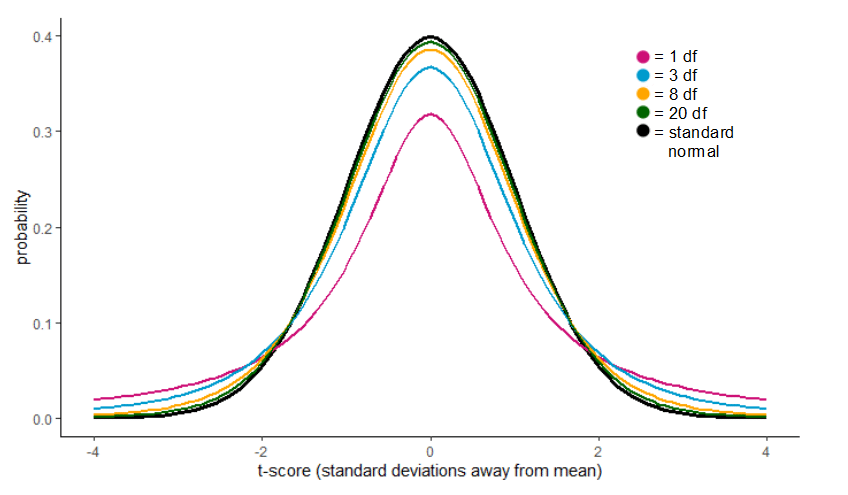
\includegraphics{diplomka obrazky/7.png}

\end{center}

Pripomína Vám to niečo? Toto t-rozdelenie je typom normálneho
rozdelenia, ktoré sa používa pri menších vzorkách. Používa sa, keď
predpokladáme, že majú dáta približne normálne rozdelenie (majú
približne bell shape, tvar zvona), avšak nepoznáme rozptyl populácie.
Odhad rozptylu t-rozdelenia záleží od veľkosti vzorky, respektíve na
stupni voľnosti. Z grafu vidíte, že ako df rastú (degree-of-freedom,
stupeň voľnosti), chvosty rozdelenia sa stenšujú a rozdelenie sa zužuje.
Stupne voľnosti vyrátame ako počet pozorovaní mínus počet premenných a
intercept. Toto rozdelenie ukazuje hustotu pravedpodobnosti, s akou sa
dané hodnoty v rozdelení môžu objaviť.

Čarovnou vlastnosťou tohto rozdelenia je, že ako rastie stupeň voľnosti,
rozdelenie sa približuje štandardnému normálnemu rozdeleniu. Štandardné
normálne rozdelenie sa vyznačuje tým, že má priemer 0 a smerodajnú
odchýlku 1.

Poďme teraz k tým juicy veciam, prečo Vám to vlastne ukazujem.

\hypertarget{t-ux161tatistika}{%
\subsection{t-štatistika}\label{t-ux161tatistika}}

Na overenie, či sme koeficient neodhadli len náhodou, ale je naozaj
významný, vyrátame t-štatistiku, ktorej formula vyzerá takto:

\[t = \frac{\hat\beta{}_i}{se(\hat\beta{}_i)}\] V t-štatistike odčítate
v čitateli vašu požadovanú hypotézu. My testujeme významnosť
\(\hat\beta{}_i\), teda či sa naša \(\hat\beta{}_i\) rovná nule a tým
pádom nie je významná. Mohli by sme to zapísať ako:

\[t = \frac{\hat\beta{}_i - \hat\beta{}_i,_0}{se(\hat\beta{}_i)}\]
Odčítame nulu, čiže sa nič nemení, a prvý zápis je úplne v poriadku.

Hej hej hej, čo je ale to se??? \emph{SE stands for standard error.}
Takže \(štandardná chyba\). Hmmmm, to neznie ako smerodajná odchýlka. A
máte pravdu! Lebo to nie je smerodajná odchýlka! Alebo, no, ono to
vlastne JE smerodajná odchýlky!

\hypertarget{sd-vs-se}{%
\subsection{SD vs SE}\label{sd-vs-se}}

Smerodajná odchýlka (standard deviaton) a štandardná chyba (standard
error).

Spomínate si na vzorec na rozptyl? Ak nie, tu ho máme:

\[s^{2} = \frac{\sum_{i=1}^{n} \left(x_{i} - \bar{x}\right)^{2}} {n-1}.\]

Všimnime si, že používame \(s^{2}\), namiesto \(\sigma^{2}\) (sigma
squared, squared = na druhú), lebo sa jedná o estimátor, kde odhadujeme
danú štatistiku (v tomto prípade rozptyl) zo vzorky. \(\sigma^{2}\) sa
používa na označenie rozptylu populácie. To máme to isté ako \(\mu\)
(mí), pre priemer populácie a \(\overline{x}\) pre priemer vzorky.

Smerodajná odchýlka je odmocnina vzorca uvedeného vyššie, základy
štatistiky, že?

\[s = \sqrt{\frac{\sum_{i=1}^{n} \left(x_{i} - \bar{x}\right)^{2}} {n-1}}.\]

Výberová smerodajná odchýlka (čiže smerodajná odchýlka vyrátaná zo
vzorky, nenechajte sa zmiesť, je to to isté ako vyššie, len sme pridali
výberová, nech sme korektní) nám určuje osciláciu hodnôt okolo priemeru,
ako veľmi sú okolo toho priemeru rozptýlené.

Štanardná chyba opisuje to isté, avšak miesto vzorky, pracuje so vzorkou
plnou priemerov. Spomeňme si na výberové rozdelenie pri náhodnom výbere.
Vezmeme vzorku, vyrátame z nej priemer a priemer dáme do šuflíka.
Vezmeme ďalšiu vzorku, vyrátame jej priemer, a aj tento priemer hodíme
do šuflíka. Toto zopakujeme veľakrát, a máme plný šuflík priemerov. Z
tejto šuplíkovej vzorky priemerov vyrátame priemer. Aaa potom vyrátame,
ako zvyšné hodnoty (priemery), oscilujú okolo priemeru vzorky. Vyrátali
sme teda smero\ldots ehm.. štandardnú chybu! Keď sa bavíme o štandardnej
chybe (SE), vieme, že sa bavíme o tom, ako natesno je súbor priemerov,
okolo priemeru. Čiže je to smerodajná odchýlka pre priemery.

\begin{quote}
\emph{V štatistike sa to beri ako odhad smerodajnej odchýlky priemeru
vzorky, okolo skutočného priemeru populácie.}
\end{quote}

Na hodine to budete rátať pomocou variačno-kovariačnej matice. My si
ukážeme všeobecný vzorec:

\[s_{\bar{X}} = \frac{s}{\sqrt{n}}\]

\begin{quote}
\emph{Vydelíme smerodajnú odchýlku vzorky, odmocninou počtu pozorovaní
vo vzorke.}
\end{quote}

Alternatívny zápis:

\[SE = \frac{s}{\sqrt{n}}\] Takže vráťme sa k našej \(t-štatistike\):

\[t = \frac{\hat\beta{}_i}{se(\hat\beta{}_i)}\]

Na jej vyrátanie použijeme odhadnutý \(\hat\beta{}_i\) koeficient, a
predelíme ho odhadnutou štandardnou chybou (ktorú pre nás vyráta R-ko do
koeficientov). Pozrime sa ešte raz na koeficienty:

\begin{Shaded}
\begin{Highlighting}[]
\KeywordTok{summary}\NormalTok{(model)}\OperatorTok{$}\NormalTok{coefficients}
\end{Highlighting}
\end{Shaded}

\begin{verbatim}
##                Estimate Std. Error   t value     Pr(>|t|)
## (Intercept) 30.09886054  1.6339210 18.421246 6.642736e-18
## data$hp     -0.06822828  0.0101193 -6.742389 1.787835e-07
\end{verbatim}

\begin{Shaded}
\begin{Highlighting}[]
\CommentTok{# Vydeľme koeficient "estimate", číslom "Std. Error" (SE),}
\CommentTok{# a pozrime sa, či nám výjde t-štatistika.}

\NormalTok{nase_t <-}\StringTok{ }\KeywordTok{summary}\NormalTok{(model)}\OperatorTok{$}\NormalTok{coefficients[}\DecValTok{1}\NormalTok{, }\DecValTok{1}\NormalTok{] }\OperatorTok{/}\StringTok{ }\KeywordTok{summary}\NormalTok{(model)}\OperatorTok{$}\NormalTok{coefficients[}\DecValTok{1}\NormalTok{, }\DecValTok{2}\NormalTok{]}

\NormalTok{nase_t}
\end{Highlighting}
\end{Shaded}

\begin{verbatim}
## [1] 18.42125
\end{verbatim}

\hypertarget{kritickuxe1-hodnota}{%
\subsection{Kritická hodnota}\label{kritickuxe1-hodnota}}

Kritická hodnota pre t-štatistiku je približne 2, že? Čo to ale značí?
Keď koeficient predelíme štandardnou chybou, rátame, koľko štandardných
chýb sa vmestí do tejto hodnoty, čiže koľko štandardných chýb je
vzdialená od tejto hodnoty. T-rozdelenie je rozdelenie pravedpobodnosti,
a čím je bližšie k stredu, tým je väčšia pravdepodobnosť výskytu. Ak si
spomínate, čo sme si vraveli pri normálnom rozdelení, že 68\% sa
nachádza v rozmedzí jednej smerodajnej odchýlky, a 95\% v rozmedzí dvoch
smerodajných odchýlok. 95\% a 2 štandardné chyby, hm, hm? Aká je
väčšinou naša hladina významnosti? 5\%! Čo je 100 - 95. A znova
opakujem, bavíme sa o rozdelení pravdepodobnosti. Ak je teda
t-štatistika väčšia ako 2, nachádzame sa ďalej ako 2 smerodajné odchýlky
od centra rozdelenia, a \textbf{pravedpodobnosť} výskytu tejto hodnoty,
je menšia ako 5\%. Šanca, že sme tento koeficient odhadli len čistou
náhodou (menej ako 5\% sa berie ako náhoda, ``by chance''), je menej ako
5\%. A teda považujeme tento koeficient za štatisticky významný.

\begin{center}

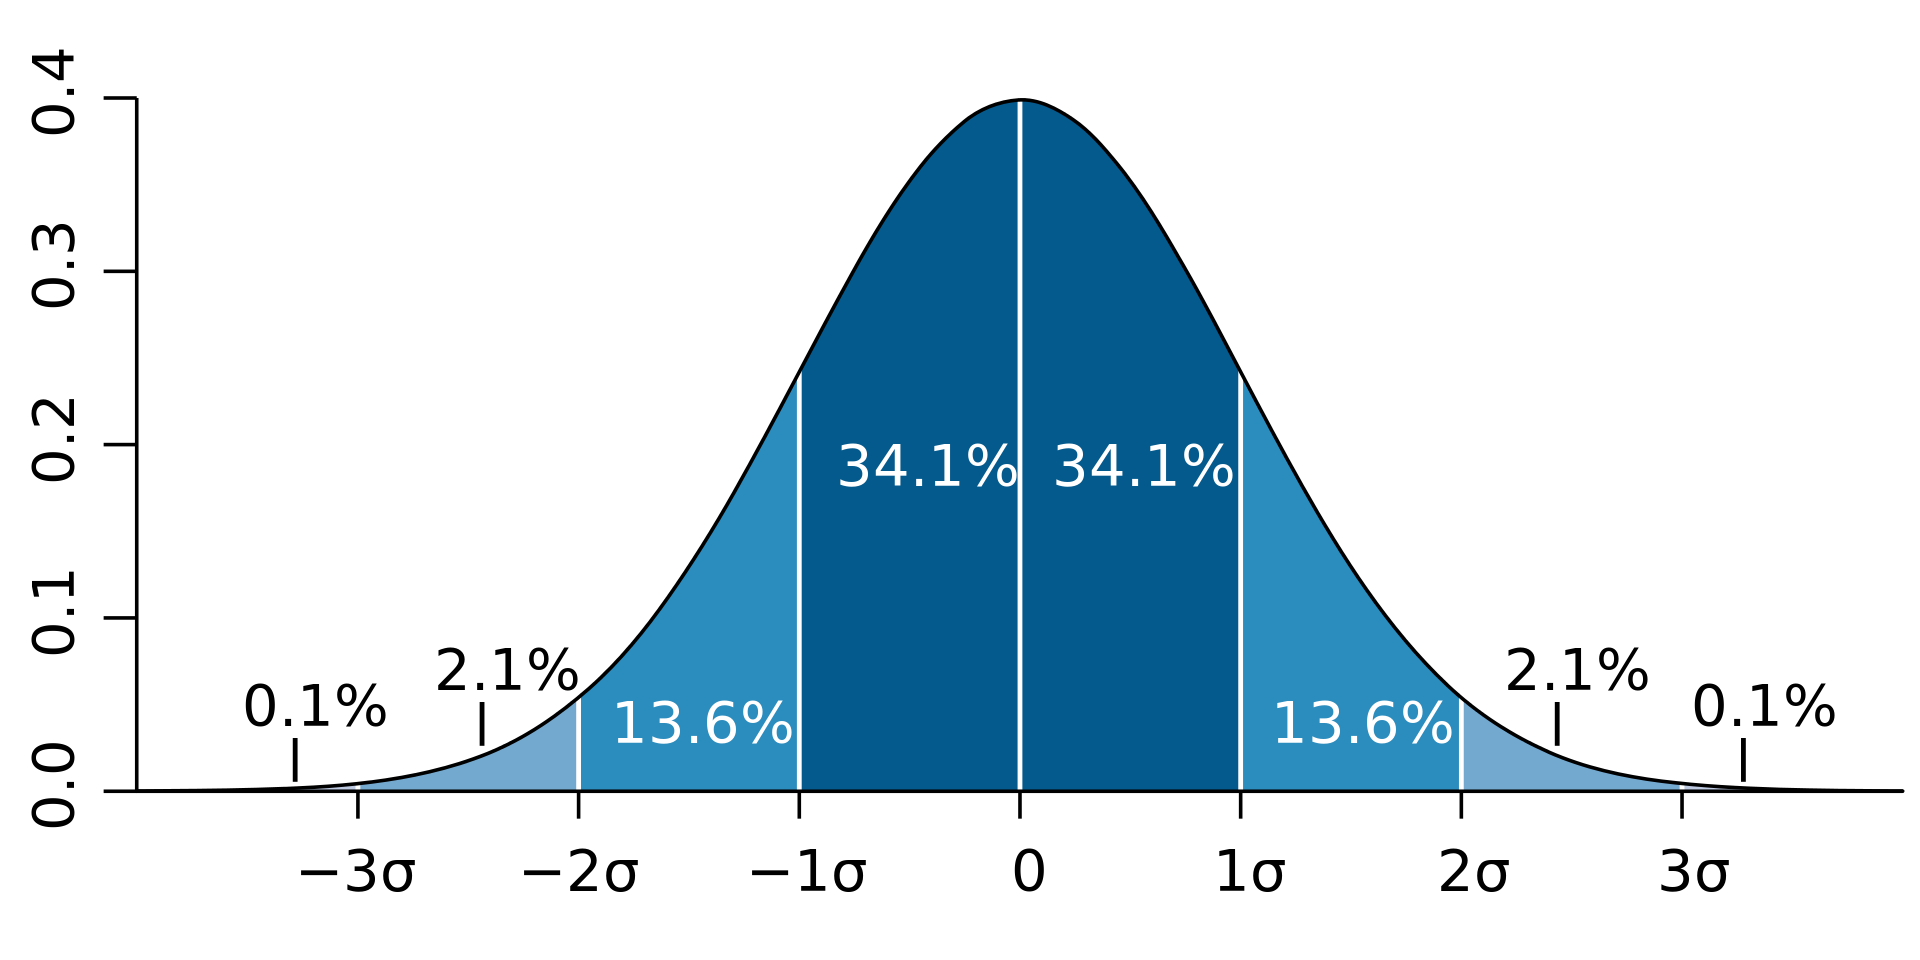
\includegraphics{diplomka obrazky/8.png}

\end{center}

\hypertarget{p-hodnota}{%
\subsection{p-hodnota}\label{p-hodnota}}

Pomocou t-štatistiky môžeme vyrátať p-hodnotu. Naša nulová hypotéza
bola:

\[H_0: \hat\beta{}_i = 0\]

Nulovú hypotézu zamietame, ak je t-štatistika väčšia ako 2, čiže sa
nachádza v chvostoch rozdelenia, inými slovami, je malá pravdepodobnosť,
že sme túto hodnotu vyrátali náhodne. A p-hodnota nevraví nič iné, ako
to, aká je pravdepodobnosť, že by sme dostali našu \(\hat\beta{}_i\)etu,
za predpokladu, že nulová hypotéza platí. p-hodnota, ukazuje
pravedpodobnosť výskytu nulovej hypotézy. Ak je táto hodnota malá,
zamietame, že \(\hat\beta{}_i\) je štatisticky nevýznamná a rovná nule.

\begin{Shaded}
\begin{Highlighting}[]
\CommentTok{# V našom prípade boli p-hodnoty 6.642736e-18, čo je veľmi malé číslo,}
\CommentTok{# 18 núl pred šestkou. Dávajte pozor, keby tam bolo e+18, tak je to obrovské}
\CommentTok{# číslo. :D Väčšinou sú malé p-hodnoty označené tromi hviezdičkami.}

\KeywordTok{summary}\NormalTok{(model)}\OperatorTok{$}\NormalTok{coefficients}
\end{Highlighting}
\end{Shaded}

\begin{verbatim}
##                Estimate Std. Error   t value     Pr(>|t|)
## (Intercept) 30.09886054  1.6339210 18.421246 6.642736e-18
## data$hp     -0.06822828  0.0101193 -6.742389 1.787835e-07
\end{verbatim}

\hypertarget{konfidenux10dnuxfd-interval}{%
\subsection{Konfidenčný interval}\label{konfidenux10dnuxfd-interval}}

Keď už sme zabŕdli do tej štatistiky, povedzme si rýchlo, čo je
konfidenčný interval. Najprv si ukážeme zápis konfidenčného intervalu
pre jednu premennú (nevravíme pre jednu preto, lebo pracujeme s
jednoduchou lineárnou regresiou, ale preto, že sa konfidenčný interval
vytvára pre každú premennú zvlášť):

\[[\hat\beta{}_i - 1.96 × SE(\hat\beta{}_i)\;\;,\;\;\hat\beta{}_i + 1.96 × SE(\hat\beta{}_i)].\]
Od odhadnutého koeficientu prv odčítame dve štandardné chyby pre určenie
spodnej hranice, a potom pričítame dve štandardné chyby pre určenie
hornej hranice.

\begin{Shaded}
\begin{Highlighting}[]
\CommentTok{# V R-ku konfidnčný interval odhadneme pomocou confint().}
\CommentTok{# Ukážeme si neskôr aj robustnú alternatívu. Zatiaľ pracujeme len s basic}
\CommentTok{# balíkmi v R.}

\KeywordTok{confint}\NormalTok{(model)}
\end{Highlighting}
\end{Shaded}

\begin{verbatim}
##                   2.5 %     97.5 %
## (Intercept) 26.76194879 33.4357723
## data$hp     -0.08889465 -0.0475619
\end{verbatim}

Interpretácia konfidenčného intervalu je nasledovná:``Ak by sme vzali
nekonečno vzoriek z populácie, v 95\% prípadov, by sa skutočný priemer
populácie nachádzal v rozmedzí 26.8 až 33.44.''

\hypertarget{vlastnosti-reziduuxed}{%
\section{Vlastnosti rezíduí}\label{vlastnosti-reziduuxed}}

Aby sme koeficienty modelu mohli použiť na štatistickú inferenciu, je
potrebné skontrolovať vlastnosti reziduí. Tieto vlastnosti sú ďalšími z
podmienok OLS metódy. Na cvičeniach sa budete venovať ich rátaniu a
ukážkach na modeloch. Ja Vám poviem, čo takéto nesplnenie vlastnosti
spôsobí, a pokúsim sa Vám to vryť do pamäti pomocou vizualizácie.
Stručne zhrniem aj využité testy a riešenia. Treba si
\textbf{zvýrazniť}, že tieto podmienky sa vzťahujú len na reziduá, a nie
na nezávislé premenné.

\hypertarget{normalita}{%
\subsection{Normalita}\label{normalita}}

Chceme, aby boli naše reziduá normálne rozdelené, čo to znamená?
Nechceme vidieť žiaden vzor správania reziduí. Reziduá majú byť
nezávisle od nezávislých premenných a s priemerom 0. Naše reziduá si
plotneme spolu s fitted, teda odhadnutými hodnotami na priamke. V prvom
grafe sme si pridali priamku, keďže reziduá by mali byť porozhadzované
názávisle po oboch stranách. Druhý graf je takzvaný QQ-plot. Reziduá sú
rozdelené normálne, ak kopírujú diagonálnu priamku, ktorú sme si
nakreslili. Tá priamka je totižto vytvorená z normálneho rozdelenia. Ak
by sme si otestovali tieto reziduá z nášho modelu, nezamietli by sme
nulovú hypotézu, reziduá teda sú rozdelené normálne-ish.

\begin{Shaded}
\begin{Highlighting}[]
\CommentTok{# My sme si tieto grafy vytvorili manuálne, dopracovali by ste sa k ním}
\CommentTok{# však aj cez funkciu plot(váš_model). Museli by ste sa k nemu však preklikať.}

\KeywordTok{par}\NormalTok{(}\DataTypeTok{mfrow=}\KeywordTok{c}\NormalTok{(}\DecValTok{1}\NormalTok{, }\DecValTok{2}\NormalTok{))}

\KeywordTok{plot}\NormalTok{(model}\OperatorTok{$}\NormalTok{fitted.values, model}\OperatorTok{$}\NormalTok{residuals, }\DataTypeTok{main =} \StringTok{"reziduá vs fitted"}\NormalTok{)}
\KeywordTok{abline}\NormalTok{(}\DecValTok{0}\NormalTok{, }\DecValTok{0}\NormalTok{)}

\KeywordTok{qqnorm}\NormalTok{(model}\OperatorTok{$}\NormalTok{residuals)}
\KeywordTok{qqline}\NormalTok{(model}\OperatorTok{$}\NormalTok{residuals)}
\end{Highlighting}
\end{Shaded}

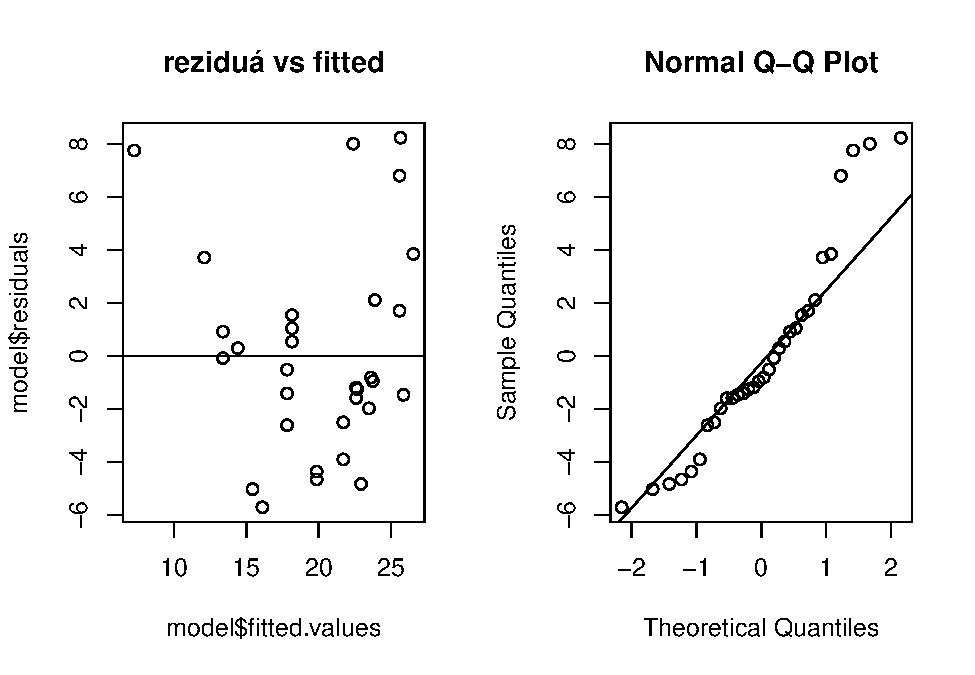
\includegraphics{test_files/figure-latex/unnamed-chunk-50-1.pdf}

Všetky podmienky, ktoré spomenieme nebudú ovplyvnovať odchýlku
koeficientu, avšak budú ovplyvňovať štandardnú chybu, teda aj
t-štatistiku a p-hodnotu. To nám znemožní správne odhadnúť štatistickú
signifikatnosť koeficientu.

Podmienka normality reziduí je jednou z tých menej závažnejších, a často
sa stane, že nie je splnená. Problémom to prestáva byť pri veľkých
vzorkách, kde začne úradovať Central limit theorem.

\hypertarget{homoskedasticita}{%
\subsection{Homoskedasticita}\label{homoskedasticita}}

Ďalšou podmienkou je konštantný rozptyl reziduí - homoskedasticita. Ak
rozptyl nie je konštantný, ale zväčšuje sa, bavíme sa o prítomnosti
heteroskedasticity. Ukážeme si to na najklasickejšom príklade, a to
vzťah príjmu a výdavkov na jedlo. Ľudia potrebujú jesť približne
rovnako, keď máte málo peňazí, nemáte veľmi na výber a všetci ľudia s
nízkym príjmom kupujú podobné množstvo a typ jedla, vynakladajú pomerne
rovnakú časť ich príjmov. Ako však príjem rastie, ľudia nezjedia
signifikantne viac, avšak môžu utrácať za omnoho drahšie potraviny, a
niekto je podobne ako ľudia s nižším príjmom. Je tam teda veľký rozptyl,
lebo ľudia s vyšším príjmom majú na výber. Pri nižšom príjme tento
rozptyl nie je, lebo keď zarobia 1000eur, nemôžu minút na potraviny 10
000eur.

\begin{Shaded}
\begin{Highlighting}[]
\CommentTok{# Vytvorme si premenné, kde X budú mzdy.}
\NormalTok{X <-}\StringTok{ }\DecValTok{1}\OperatorTok{:}\DecValTok{500}
\NormalTok{Y <-}\StringTok{ }\KeywordTok{rnorm}\NormalTok{(}\DataTypeTok{n =} \DecValTok{500}\NormalTok{, }\DataTypeTok{mean =}\NormalTok{ X, }\DataTypeTok{sd =} \FloatTok{0.6} \OperatorTok{*}\StringTok{ }\NormalTok{X)}
\NormalTok{mzdy_jedlo <-}\StringTok{ }\KeywordTok{lm}\NormalTok{(Y }\OperatorTok{~}\StringTok{ }\NormalTok{X)}

\KeywordTok{plot}\NormalTok{(}\DataTypeTok{x =}\NormalTok{ X, }\DataTypeTok{y =}\NormalTok{ Y, }\DataTypeTok{xlab =} \StringTok{"príjem"}\NormalTok{, }\DataTypeTok{ylab =} \StringTok{"výdaje na jedlo"}\NormalTok{,}
     \DataTypeTok{main =} \StringTok{"vzťah príjmu a výdavkov na jedlo"}\NormalTok{)}

\KeywordTok{abline}\NormalTok{(mzdy_jedlo, }\DataTypeTok{col =} \StringTok{"red"}\NormalTok{)}
\end{Highlighting}
\end{Shaded}

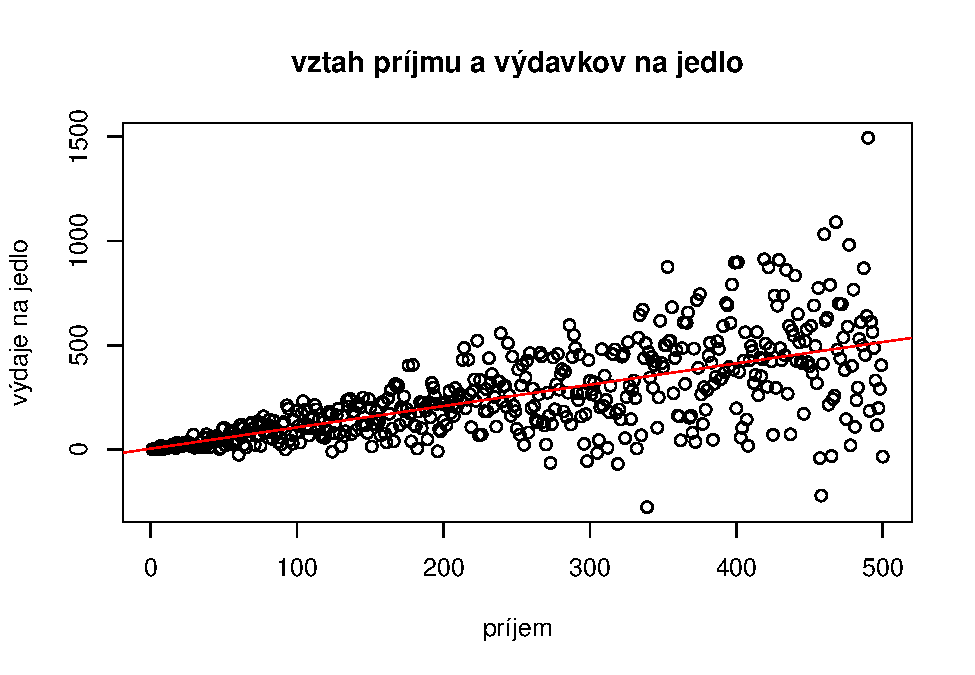
\includegraphics{test_files/figure-latex/unnamed-chunk-51-1.pdf}

Prítomnosť heteroskedasticity \textbf{zmenší} štandardnú chybu,
dostaneme menšie hodnoty, než by sme mali. To môže viesť k označeniu
koeficientu za štatisticky signifikantný, aj keď to nebude pravda.

Heteroskedasticitu môžeme detekovať pomocou:

\begin{itemize}
\tightlist
\item
  vizualizácie,
\item
  Breusch-Pagan testu,
\item
  Goldfeld-Quandt testu.
\end{itemize}

A vyriešiť napríklad pomocou:

\begin{itemize}
\tightlist
\item
  robustných metód na odhad štandardných chýb,
\item
  vážených najmenších štvorcov (WLS),
\item
  logaritmickej transformácie modelu.
\end{itemize}

\hypertarget{autokoreluxe1cia}{%
\subsection{Autokorelácia}\label{autokoreluxe1cia}}

Autokorelácia, alebo sériová korelácia znamená, keď vieme predpovedať
pohyb zvyšku pomocou iného zvyšku. Takže reziduá od seba nie sú
nezávislé. Takýto problém sa častejšie vyskytuje v časových radoch. Môže
to byť spôsobené Odchýlkou vynechanej premennej alebo nesprávnou
špecifikáciou modelu. Aj tento neduh je možné analyzovať buď vizuálne
alebo testami. Samozrejme testy sú omnoho spoľahlivejie. My si ale
ukážeme ako taká autokorelácia vyzerá.

\begin{center}

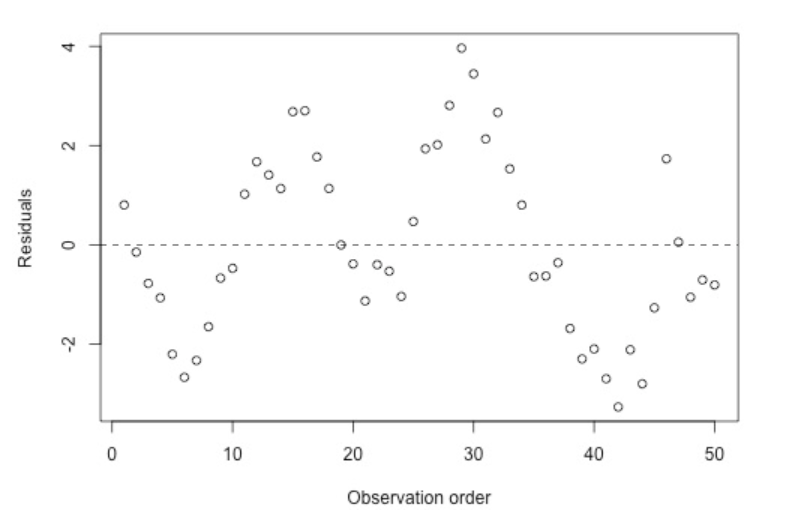
\includegraphics{diplomka obrazky/9.png}

\end{center}

\begin{Shaded}
\begin{Highlighting}[]
\CommentTok{# Šikovnou funkciou na skontrolovanie autokorelácie je acf().}
\CommentTok{# Cool trik je, ak chcete nový riadok v názvoch, použite "\textbackslash{}n".}

\KeywordTok{acf}\NormalTok{(model}\OperatorTok{$}\NormalTok{residuals, }\DataTypeTok{main =} \StringTok{"do funkcie vložíme }\CharTok{\textbackslash{}n}\StringTok{ klasicky reziduá"}\NormalTok{)}
\end{Highlighting}
\end{Shaded}

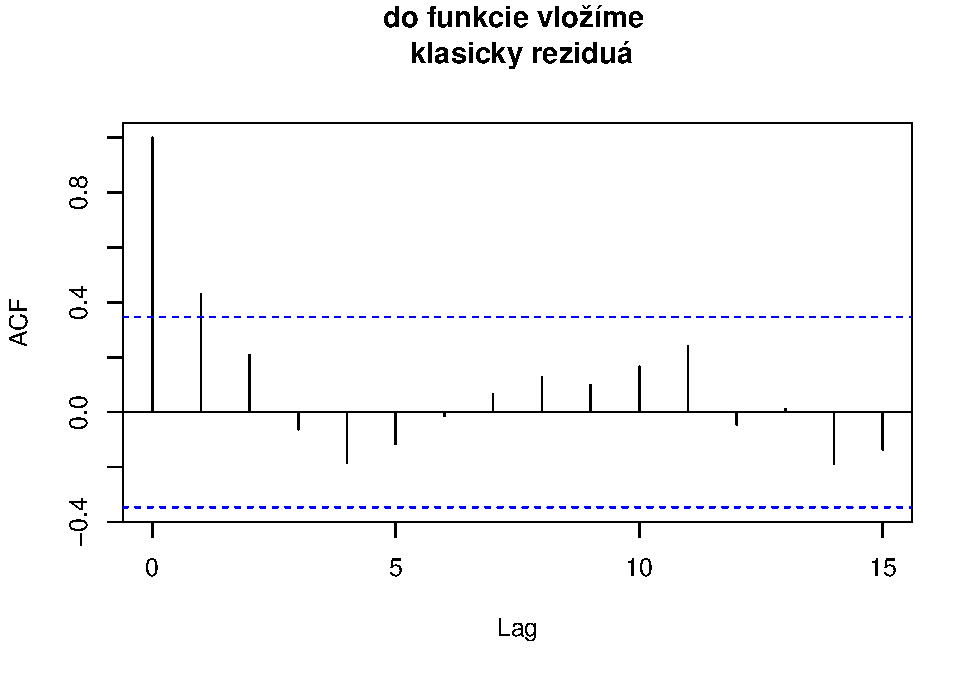
\includegraphics{test_files/figure-latex/unnamed-chunk-52-1.pdf}

\begin{Shaded}
\begin{Highlighting}[]
\CommentTok{# Samozrejme v prvom stĺpci bude korelácia jedna, lebo korelujeme samého seba.}
\CommentTok{# Ak sú korelácia nepresahuje za čiary, reziduá nie sú silne korelované a }
\CommentTok{# autokorelácia, resp. sériová korelácia, nie je prítomná.}
\end{Highlighting}
\end{Shaded}

Problémy nám to spôsobí podobné ako heteroskedasticita, okrem iného však
môže ovplyvniť aj hodnotu \(R^2\). Autokoreláciu môžeme detekovať
pomocou:

\begin{itemize}
\tightlist
\item
  Durbin-Watson testu,
\item
  Breusch-Godfrey testu.
\end{itemize}

A vyriešiť pomocou:

\begin{itemize}
\tightlist
\item
  robustných metód na odhad štandardných chýb,
\item
  doplnenia vynechanej premennej,
\item
  opravenia funkčnej formy modelu,
\item
  využitia prvých diferencií,
\item
  použitia dummy premenných.
\end{itemize}

\hypertarget{multikolinearita}{%
\subsection{Multikolinearita}\label{multikolinearita}}

Multikolinearita sa vyskytuje len vo viacnásobnej regresií, keďže sa
jedná o koreláciu medzi dvoma nezávislými premennými. Korelácia medzi
závislou a nezávislou premennou je žiaduca. Poznáme dokonalú a
nedokonalú multikolinearitu. Pri dokonalej dokážeme jednu nezávislú
premennú vyjadriť lineárnou kombináciou inej premennej. V takomto
prípade nám väčšinou ani počítač nebude chcieť model vyrátať. Nás
väčšinou trápi nedokonalá, kde sú premenné vysoko korelované. Prečo je
to problém? AK sú premenné korelované, nedokážeme dobre odhadnúť
koeficient, keďže pri každej pridanej alebo odobranej premennej, má
koeficient tendenciu sa meniť a to vo väčšej miere. Inak povedané, je
problém dostatočne odizolovať koeficient. Koeficienty sú tak citlivé na
zmenu premenných. Ďalším problémom je, že štandardné chyby nám riadne
narastú, čím môžu označiť štatisticky signifikantné premenné za
nesignifikantné. \(R^2\) a F-test však nezvyknú byť ovplyvnené.

Multikolinearitu je možné detekovať pomocou:

\begin{itemize}
\tightlist
\item
  korelačnej matice,
\item
  VIF test,
\item
  analýzy determinantu matice,
\item
  parciálnych korelačných koeficientov.
\end{itemize}

A vyriešiť pomocou:

\begin{itemize}
\tightlist
\item
  odstránenia jednej z korelovaných premenných,
\item
  skombinovanie premenných,
\item
  neurobiť nič.
\end{itemize}

Niekedy je možné premennú ponechať v modeli, ak našim cieľom nie je
použiť ju na interpretovanie, ale len ako kontrolnú premennú, alebo keď
korelácia nie je neúnosne vysoká (0.9 a viac).


\end{document}




% !TeX encoding = UTF-8
% !TeX spellcheck = sk_SK
% !TeX root=tukedip.tex
%%
\begin{thebibliography}{19}
\addcontentsline{toc}{section}{\numberline{}Zoznam použitej
literatúry}

\harvarditem{Barančok et al.}{1995}{barancok}
BARANČOK, D. et al. 1995. \emph{The effect of semiconductor surface
treatment on LB film/Si interface.} In:~Physica Status Solidi (a), 
ISSN 0031-8965, 1995, vol. 108, no.~2, \mbox{pp. K~87--90}

\harvarditem{Benčo}{2001}{benco}
BENČO, J. 2001. \emph{Metodológia vedeckého výskumu.} Bratislava~:
IRIS, 2001, ISBN 80\discretionary{-}{-}{-}89018-27-0

\harvarditem{Gonda}{2001}{gonda}
GONDA, V. 2001. \emph{Ako napísať a~úspešne obhájiť diplomovú prácu.}
Bratislava~: Elita, 2001, 3. doplnené a~prepracované vydanie, 120~s.
ISBN 80-8044-075-1

\harvarditem{Jadr. fyz. a~tech.}{1985}{slovnik}
\emph{Jadrová fyzika a~technika: Terminologický výkladový slovník.}
2.~rev.~vyd. Bratislava~: ALFA, 1985. 235~s. ISBN 80-8256-030-5

\harvarditem{Katuščák}{1998}{kat}
KATUŠČÁK, D. 1998. \emph{Ako písať vysokoškolské a~kvalifikačné
práce.} Bratislava~: Stimul, 1998, 2.~doplnené vydanie. 121~s. ISBN
80-85697-82-3

\harvarditem{Lamoš a~Potocký}{1989}{lamos}
LAMOŠ, F. -- POTOCKÝ, R. 1989. \emph{Pravdepodobnosť a~matematická
štatistika.} 1.~vyd. Bratislava~: Alfa, 1989. 344~s. ISBN 80-8046-020-5

\harvarditem{Sýkora a~i.}{1980}{sykora}
SÝKORA, F. a~iní. 1980. \emph{Telesná výchova a~šport.} 1.vyd.
Bratislava~: SPN, 1980. 35~s. ISBN 80-8046-020-5

\harvarditem{Steinerová}{2000}{steinerova}
STEINEROVÁ, J. 2000. \emph{Základy filozofie človeka v~knižničnej
a~informačnej vede.} In:~Kimlička, Š., Knižničná a~informačná veda na
prahu informačnej spoločnosti. Bratislava~: Stimul, 2000. ISBN
80-2274-035-2, s. 327--334

\harvarditem{Šumichrast}{1995}{sumichrast}
ŠUMICHRAST, Ľ. 1995. \emph{On the performance of higher approximations
of radiation boundary conditions for the simulation of wave propagation
in structures of integrated optics.} In:~Photonics '95. Prague~: CTU,
1995, pp. 159--161

\harvarditem{Šumichrast}{1995}{sumichras}
ŠUMICHRAST, Ľ. 1995. \emph{On the performance of higher approximations
	of radiation boundary conditions for the simulation of wave propagation
	in structures of integrated optics.} In:~Photonics '95. Prague~: CTU,
1995, pp. 159--161

\end{thebibliography}
%
\section*{Zoznam pr\'iloh}
\addcontentsline{toc}{section}{\numberline{}Zoznam pr\'iloh}
\thispagestyle{empty}

\begin{description}
	\item[Príloha A] CD médium -- záverečná práca v~elektronickej podobe.
\end{description}
%
% !TeX root=tukedip.tex
% !TeX encoding = UTF-8
% !TeX spellcheck = sk_SK
\section*{Príloha A}
\addcontentsline{toc}{section}{\numberline{}Príloha A}
\subsection*{Prílohy}

Táto časť záverečnej práce je povinná a~obsahuje zoznam všetkých
príloh vrátane elektronických nosičov. Názvy príloh v~zozname musia
byť zhodné s~názvami uvedenými na príslušných prílohách. Tlačené
prílohy majú na prvej strane identifikačné údaje -- informácie zhodné
s~titulnou stranou záverečnej práce doplnené o~názov príslušnej
prílohy. Identifikačné údaje sú aj na priložených diskoch alebo
disketách. Ak je médií viac, sú označené aj číselne v~tvare $I/N$, kde
$I$ je poradové číslo a~$N$ je celkový počet daných médií. Zoznam
príloh má nasledujúci tvar:
\begin{description}
\item[Príloha A] CD médium -- záverečná práca v~elektronickej podobe,
prílohy v~elektronickej podobe.
\item[Príloha B] Používateľská príručka
\item[Príloha C] Systémová príručka
\end{description}
Prílohová časť je samostatnou časťou kvalifikačnej práce. Každá
príloha začína na novej strane a je označená samostatným písmenom
(Príloha A, Príloha B, \dots). Číslovanie strán príloh nadväzuje na
číslovanie strán v~hlavnom texte. Pri každej prílohe sa má uviesť
prameň, z~ktorého sme príslušný materiál získali.
%
% !TeX root=tukedip.tex
% !TeX encoding = UTF-8
% !TeX spellcheck = sk_SK
\section*{Príloha B}
\addcontentsline{toc}{section}{\numberline{}Príloha B}
\subsection*{Bibliografické odkazy}

Táto časť záverečnej práce je povinná. V~zozname použitej literatúry
sa uvádzajú odkazy podľa normy STN~ISO~690--2 (01 0197) (Informácie
a~dokumentácia. Bibliografické citácie. Časť 2: Elektronické
dokumenty alebo ich časti, dátum vydania 1.~12.~2001, ICS:~01.140.20).
Odkazy sa môžu týkať knižných, časopiseckých a~iných zdrojov
informácií (zborníky z~konferencií, patentové dokumenty, normy,
odporúčania, kvalifikačné práce, osobná korešpondencia a~rukopisy,
odkazy cez sprostredkujúci zdroj, elektronické publikácie), ktoré boli
v~záverečnej práci použité.

Forma citácií sa zabezpečuje niektorou z~metód, opísaných v~norme
STN~ISO~690, 1998, s.~21. Podrobnejšie informácie nájdete na stránke
\texttt{http://www.tuke.sk/anta/} v~záložke {\small\sf Výsledky
práce/Prehľad normy pre publikovanie STN~ISO~690 a~STN~ISO~690-2}.

Existujú dva hlavné spôsoby citovania v~texte.

\begin{itemize}
\item Citovanie podľa mena a~dátumu.
\item Citovanie podľa odkazového čísla.
\end{itemize}

\emph{Preferovanou metódou citovania} v~texte vysokoškolskej
a~kvalifikačnej práce je podľa normy ISO~7144 citovanie podľa mena
a~dátumu \citep{kat,gonda}. V~tomto prípade sa zoznam použitej
literatúry upraví tak, že za meno sa pridá rok vydania. Na uľahčenie
vyhľadávania citácií sa zoznam vytvára v~abecednom poradí autorov.

\medskip

Príklad:
\dots podľa \citep{steinerova} je táto metóda dostatočne rozpracovaná
na to, aby mohla byť všeobecne používaná v~\dots

\medskip

Druhý spôsob uvedenia odkazu na použitú literatúru je uvedenie len
čísla tohto zdroja v~hranatých zátvorkách bez mena autora (autorov)
najčastejšie na konci príslušnej vety alebo odstavca.

\medskip

Príklad:
\dots podľa [13] je táto metóda dostatočne rozpracovaná na to, aby
mohla byť všeobecne používaná v~\dots ako je uvedené v~[14].

\medskip

Citácie sú spojené s~bibliografickým odkazom poradovým číslom v~tvare
indexu alebo čísla v~hranatých zátvorkách. Odkazy v~zozname na konci
práce budú usporiadané podľa týchto poradových čísel. Viacero citácií
toho istého diela bude mať rovnaké číslo. Odporúča sa usporiadať
jednotlivé položky v~poradí citovania alebo podľa abecedy.

\medskip
\noindent
Rôzne spôsoby odkazov je možné dosiahnuť zmenou voľby v~balíku
\verb+natbib+:

\noindent
\verb+% Citovanie podla mena autora a roku+\\
\verb+\usepackage[]{natbib}\citestyle{chicago}+\\
\verb+% Možnosť rôznych štýlov citácií. Príklady sú uvedené+\\
\verb+% v preambule súboru natbib.sty.+\\
\verb+% Napr. štýly chicago, egs, pass, anngeo, nlinproc produkujú+\\
\verb+% odkaz v tvare (Jones, 1961; Baker, 1952). V prípade, keď+\\
\verb+% neuvedieme štýl citácie (vynecháme \citestyle{}) v "options"+\\
\verb+% balíka natbib zapíšeme voľbu "colon".+

\medskip
\noindent
Keď zapneme voľbu \verb+numbers+, prepneme sa do režimu citovania
podľa odkazového čísla.

\noindent
\verb+% Metoda ciselnych citacii+\\
\verb+\usepackage[numbers]{natbib}+

\bigskip

Pri zápise odkazov sa používajú nasledujúce pravidlá:

V~odkaze na knižnú publikáciu (pozri príklad zoznamov na konci tejto
časti):
\begin{itemize}
\item Uvádzame jedno, dve alebo tri prvé mená oddelené pomlčkou,
ostatné vynecháme a~namiesto nich napíšeme skratku et al. alebo a~i.
\item Podnázov sa môže zapísať vtedy, ak to uľahčí identifikáciu
dokumentu. Od názvu sa oddeľuje dvojbodkou a~medzerou.
\item Dlhý názov sa môže skrátiť v~prípade, ak sa tým nestratí
podstatná informácia. Nikdy sa neskracuje začiatok názvu. Všetky
vynechávky treba označiť znamienkami vypustenia  \uv{\dots}
\end{itemize}

Pri využívaní informácií z~elektronických dokumentov  treba
dodržiavať tieto zásady:
\begin{itemize}
\item  uprednostňujeme autorizované súbory solídnych služieb
a~systémov,
\item zaznamenáme dostatok informácií o~súbore tak, aby ho bolo opäť
možné vyhľadať,
\item urobíme si kópiu použitého prameňa v~elektronickej alebo
papierovej forme,
\item za verifikovateľnosť informácií zodpovedá autor, ktorý sa na
ne odvoláva.
\end{itemize}

Pre zápis elektronických dokumentov platia tie isté pravidlá, ako pre
zápis \uv{klasických}. Navyše treba uviesť tieto údaje:
\begin{itemize}
\item  druh nosiča  [online], [CD-ROM], [disketa], [magnetická páska]
\item dátum citovania  (len pre online dokumenty)
\item dostupnosť  (len pre online dokumenty)
\end{itemize}

Poradie prvkov odkazu je nasledovné:
Autor. Názov. In Názov primárneho zdroja: Podnázov. [Druh  nosiča].
Editor. Vydanie alebo verzia. Miesto vydania : Vydavateľ, dátum
vydania. [Dátum citovania]. Poznámky.  Dostupnosť. ISBN alebo ISSN.
%
% !TeX encoding = UTF-8
% !TeX spellcheck = sk_SK
% !TeX root=tukedip.tex
\section*{Príloha C}
\addcontentsline{toc}{section}{\numberline{}Príloha C}
\subsection*{Vytvorenie zoznamu skratiek a symbolov}

Ak sú v~práci skratky a symboly, vytvára sa \emph{Zoznam skratiek
a~symbolov} (a~ich dešifrovanie). V~prostredí \LaTeX{}u sa takýto
zoznam
ľahko vytvorí pomocou balíka \verb+nomencl+. Postup je nasledovný:
\begin{enumerate}
\item Do preambuly zapíšeme nasledujúce príkazy\\
\verb+\usepackage[slovak,noprefix]{nomencl}+\\ \verb+\makeglossary+
\item  V~mieste, kde má byť vložený zoznam zapíšeme príkaz\\
\verb+\printglossary+
\item V miestach, kde sa vyskytujú skratky a symboly ich definíciu
zavedieme, napr. ako     	v~našom texte, príkazmi\\
\verb+\nomenclature{$\upmu$}{mikro, $10^{-6}$}+\\
\verb+\nomenclature{V}{volt, základná jednotka napätia v sústave SI}+\\
a dokument \uv{pre\LaTeX{}ujeme}.
\item Z~príkazového riadka spustíme program \verb+makeindex+
s~prepínačmi podľa použitého operačného systému, napr.~v~OS~GNU/Linux
s~distribúciou Ubuntu~$10.04$ a~verziou \verb+texlive 2009-7+
napíšeme:\\
\verb*+makeindex tukedip.glo -s nomencl.ist -o tukedip.gls+\\
~v~OS~Win\,XP s~verziou \verb+TeXLive 2010+
napíšeme:\\
\verb*+makeindex -o tukedip.gls -s nomencl.ist tukedip.glo+

\item Po opätovnom \uv{pre\LaTeX{}ovaní} dokumentu sa na
požadované
miesto vloží \emph{Zoznam skratiek a symbolov}.
\end{enumerate}


\newpage
\phantomsection
\protect\label{page:posledna}

\end{document}

